\documentclass[conference]{IEEEtran}
\IEEEoverridecommandlockouts
% The preceding line is only needed to identify funding in the first footnote. If that is unneeded, please comment it out.
\usepackage{cite}
\usepackage{amsmath,amssymb,amsfonts}
\usepackage{algorithmic}
\usepackage{graphicx}
\usepackage{textcomp}
\usepackage{cite}
\usepackage{algorithmic}
\usepackage{graphicx}
\usepackage{textcomp}
\usepackage[dvipsnames]{xcolor}
\usepackage{paralist}
\usepackage[inline]{enumitem}
\usepackage{caption}
\usepackage{multirow}
\usepackage{booktabs}
\usepackage{makecell}
\usepackage{tabu, booktabs}
\usepackage{float}
\usepackage{subcaption}
\usepackage{pifont}
\usepackage{comment}
\usepackage{todonotes}
\usepackage{hyperref}
\usepackage{csquotes}
\usepackage{multirow}
\usepackage{booktabs}
\usepackage{graphicx}
\usepackage{epstopdf}
\usepackage{color}
\usepackage{gnuplottex}
\usepackage{graphicx}
\usepackage{epstopdf}
\usepackage{pgf}


\newcommand\myshade{85}

\pdfobjcompresslevel=0
\pdfminorversion=4


\definecolor{magma_darker}{HTML}{fdc38a}
\definecolor{magma_dark}{HTML}{e15666}
% \definecolor{magma_light}{HTML}{82s247f}
\definecolor{magma_lighter}{HTML}{1f0c43}

\definecolor{cvpr_link}{HTML}{00ffff}
\definecolor{cvpr_cite}{HTML}{00ff00}
\definecolor{cvpr_file}{HTML}{ff0000}

\definecolor{royalblue}{RGB}{65, 105, 225}
\definecolor{darkgreen}{RGB}{0, 100, 0}
\definecolor{darkred}{RGB}{139, 0, 0}
\definecolor{darkviolet}{RGB}{148, 0, 211}

\colorlet{linkColor}{violet}
\colorlet{citeColor}{YellowOrange}
\colorlet{urlColor}{Emerald}

\hypersetup{
  linkcolor  = darkviolet!\myshade!black,
  citecolor  = citeColor!\myshade!black,
  urlcolor   = urlColor!\myshade!black,
  filecolor  = darkgreen!\myshade!black,
  colorlinks = true,
}
\usepackage[a4paper, total={184mm,239mm}]{geometry}
\def\BibTeX{{\rm B\kern-.05em{\sc i\kern-.025em b}\kern-.08em
    T\kern-.1667em\lower.7ex\hbox{E}\kern-.125emX}}

\ExplSyntaxOn
\DeclareExpandableDocumentCommand{\convertlen}{ O{cm} m }
 {
  \dim_to_decimal_in_unit:nn { #2 } { 1 #1 } cm
 }
\ExplSyntaxOff
\usepackage{gnuplottex}
\usepackage{tikz}
\usepackage{mathtools}
\newcommand{\ra}[1]{\renewcommand{\arraystretch}{#1}}
\usetikzlibrary{matrix,calc,positioning,arrows.meta}

\newcommand{\omark}{\ding{51}}
\newcommand{\cmark}{\ding{52}}

\DeclarePairedDelimiter\ceil{\lceil}{\rceil}
\DeclarePairedDelimiter\floor{\lfloor}{\rfloor}

\DeclareMathOperator*{\argmax}{arg\,max}
\DeclareMathOperator*{\argmin}{arg\,min}

\newcommand{\abs}[1]{\lvert#1\rvert}
\newcommand{\Abs}[1]{\left\lvert#1\right\rvert}

\newcommand{\deriv}[2][x]{\frac{\mathrm{d}#2}{\mathrm{d}#1}}
\newcommand{\adj}[1]{\mathrm{adj}(#1)}
\newcommand{\spec}[1]{\mathrm{spec}(#1)}
\newcommand{\diag}[1]{\mathrm{diag}(#1)}
\newcommand{\tril}[1]{\mathrm{tril}(#1)}
\newcommand{\triu}[1]{\mathrm{triu}(#1)}
\newcommand{\chol}[1]{\mathrm{chol}(#1)}
\newcommand{\sinc}[1]{\mathrm{sinc}\left(#1\right)}

\newcommand{\stimes}{{\times}}

\newcommand*\circled[1]{\tikz[baseline=(char.base)]{\node[shape=circle,fill,inner sep=0.5pt] (char) {\textcolor{white}{#1}};}}
\newcommand*\pilar[3]{\tikz[baseline=(char.base)]{\node[shape=circle,fill=#2,inner sep=0.5pt] (char) {\textcolor{#3}{#1}};}}

\newcommand\norm[1]{\left\lVert#1\right\rVert}

\newcommand{\red}[1]{{\color{red}#1}}
\newcommand{\blue}[1]{{\color{blue}#1}}

% If your conference documentclass or package defines these macros,
% change these macros to different names.
\newcommand*{\affaddr}[1]{#1} % No op here. Customize it for different styles.
\newcommand*{\affmark}[1][*]{\textsuperscript{#1}}
\newcommand*{\email}[1]{#1}
\setlength {\marginparwidth }{2cm}
\begin{document}

\title{Late Breaking Results: Leveraging Approximate Computing for Carbon-Aware DNN Accelerators}

\author{
\IEEEauthorblockN{
Aikaterini Maria Panteleaki\IEEEauthorrefmark{1},
Konstantinos Balaskas\IEEEauthorrefmark{2},
Georgios Zervakis\IEEEauthorrefmark{2},
Hussam Amrouch\IEEEauthorrefmark{3},
Iraklis Anagnostopoulos\IEEEauthorrefmark{1}
}
\IEEEauthorblockA{
\IEEEauthorrefmark{1}Southern Illinois University Carbondale, 
\IEEEauthorrefmark{2}University of Patras, 
\IEEEauthorrefmark{3}Technical University of Munich
}
}

\maketitle
\begin{abstract}  
Test time scaling is currently one of the most active research areas that shows promise after training time scaling has reached its limits.
Deep-thinking (DT) models are a class of recurrent models that can perform easy-to-hard generalization by assigning more compute to harder test samples.
However, due to their inability to determine the complexity of a test sample, DT models have to use a large amount of computation for both easy and hard test samples.
Excessive test time computation is wasteful and can cause the ``overthinking'' problem where more test time computation leads to worse results.
In this paper, we introduce a test time training method for determining the optimal amount of computation needed for each sample during test time.
We also propose Conv-LiGRU, a novel recurrent architecture for efficient and robust visual reasoning. 
Extensive experiments demonstrate that Conv-LiGRU is more stable than DT, effectively mitigates the ``overthinking'' phenomenon, and achieves superior accuracy.
\end{abstract}  

\begin{IEEEkeywords}
Approximate Accelerators, Embodied Carbon Footprint, Sustainable Computing
\end{IEEEkeywords}

\section{Introduction}
\label{sec:introduction}
The business processes of organizations are experiencing ever-increasing complexity due to the large amount of data, high number of users, and high-tech devices involved \cite{martin2021pmopportunitieschallenges, beerepoot2023biggestbpmproblems}. This complexity may cause business processes to deviate from normal control flow due to unforeseen and disruptive anomalies \cite{adams2023proceddsriftdetection}. These control-flow anomalies manifest as unknown, skipped, and wrongly-ordered activities in the traces of event logs monitored from the execution of business processes \cite{ko2023adsystematicreview}. For the sake of clarity, let us consider an illustrative example of such anomalies. Figure \ref{FP_ANOMALIES} shows a so-called event log footprint, which captures the control flow relations of four activities of a hypothetical event log. In particular, this footprint captures the control-flow relations between activities \texttt{a}, \texttt{b}, \texttt{c} and \texttt{d}. These are the causal ($\rightarrow$) relation, concurrent ($\parallel$) relation, and other ($\#$) relations such as exclusivity or non-local dependency \cite{aalst2022pmhandbook}. In addition, on the right are six traces, of which five exhibit skipped, wrongly-ordered and unknown control-flow anomalies. For example, $\langle$\texttt{a b d}$\rangle$ has a skipped activity, which is \texttt{c}. Because of this skipped activity, the control-flow relation \texttt{b}$\,\#\,$\texttt{d} is violated, since \texttt{d} directly follows \texttt{b} in the anomalous trace.
\begin{figure}[!t]
\centering
\includegraphics[width=0.9\columnwidth]{images/FP_ANOMALIES.png}
\caption{An example event log footprint with six traces, of which five exhibit control-flow anomalies.}
\label{FP_ANOMALIES}
\end{figure}

\subsection{Control-flow anomaly detection}
Control-flow anomaly detection techniques aim to characterize the normal control flow from event logs and verify whether these deviations occur in new event logs \cite{ko2023adsystematicreview}. To develop control-flow anomaly detection techniques, \revision{process mining} has seen widespread adoption owing to process discovery and \revision{conformance checking}. On the one hand, process discovery is a set of algorithms that encode control-flow relations as a set of model elements and constraints according to a given modeling formalism \cite{aalst2022pmhandbook}; hereafter, we refer to the Petri net, a widespread modeling formalism. On the other hand, \revision{conformance checking} is an explainable set of algorithms that allows linking any deviations with the reference Petri net and providing the fitness measure, namely a measure of how much the Petri net fits the new event log \cite{aalst2022pmhandbook}. Many control-flow anomaly detection techniques based on \revision{conformance checking} (hereafter, \revision{conformance checking}-based techniques) use the fitness measure to determine whether an event log is anomalous \cite{bezerra2009pmad, bezerra2013adlogspais, myers2018icsadpm, pecchia2020applicationfailuresanalysispm}. 

The scientific literature also includes many \revision{conformance checking}-independent techniques for control-flow anomaly detection that combine specific types of trace encodings with machine/deep learning \cite{ko2023adsystematicreview, tavares2023pmtraceencoding}. Whereas these techniques are very effective, their explainability is challenging due to both the type of trace encoding employed and the machine/deep learning model used \cite{rawal2022trustworthyaiadvances,li2023explainablead}. Hence, in the following, we focus on the shortcomings of \revision{conformance checking}-based techniques to investigate whether it is possible to support the development of competitive control-flow anomaly detection techniques while maintaining the explainable nature of \revision{conformance checking}.
\begin{figure}[!t]
\centering
\includegraphics[width=\columnwidth]{images/HIGH_LEVEL_VIEW.png}
\caption{A high-level view of the proposed framework for combining \revision{process mining}-based feature extraction with dimensionality reduction for control-flow anomaly detection.}
\label{HIGH_LEVEL_VIEW}
\end{figure}

\subsection{Shortcomings of \revision{conformance checking}-based techniques}
Unfortunately, the detection effectiveness of \revision{conformance checking}-based techniques is affected by noisy data and low-quality Petri nets, which may be due to human errors in the modeling process or representational bias of process discovery algorithms \cite{bezerra2013adlogspais, pecchia2020applicationfailuresanalysispm, aalst2016pm}. Specifically, on the one hand, noisy data may introduce infrequent and deceptive control-flow relations that may result in inconsistent fitness measures, whereas, on the other hand, checking event logs against a low-quality Petri net could lead to an unreliable distribution of fitness measures. Nonetheless, such Petri nets can still be used as references to obtain insightful information for \revision{process mining}-based feature extraction, supporting the development of competitive and explainable \revision{conformance checking}-based techniques for control-flow anomaly detection despite the problems above. For example, a few works outline that token-based \revision{conformance checking} can be used for \revision{process mining}-based feature extraction to build tabular data and develop effective \revision{conformance checking}-based techniques for control-flow anomaly detection \cite{singh2022lapmsh, debenedictis2023dtadiiot}. However, to the best of our knowledge, the scientific literature lacks a structured proposal for \revision{process mining}-based feature extraction using the state-of-the-art \revision{conformance checking} variant, namely alignment-based \revision{conformance checking}.

\subsection{Contributions}
We propose a novel \revision{process mining}-based feature extraction approach with alignment-based \revision{conformance checking}. This variant aligns the deviating control flow with a reference Petri net; the resulting alignment can be inspected to extract additional statistics such as the number of times a given activity caused mismatches \cite{aalst2022pmhandbook}. We integrate this approach into a flexible and explainable framework for developing techniques for control-flow anomaly detection. The framework combines \revision{process mining}-based feature extraction and dimensionality reduction to handle high-dimensional feature sets, achieve detection effectiveness, and support explainability. Notably, in addition to our proposed \revision{process mining}-based feature extraction approach, the framework allows employing other approaches, enabling a fair comparison of multiple \revision{conformance checking}-based and \revision{conformance checking}-independent techniques for control-flow anomaly detection. Figure \ref{HIGH_LEVEL_VIEW} shows a high-level view of the framework. Business processes are monitored, and event logs obtained from the database of information systems. Subsequently, \revision{process mining}-based feature extraction is applied to these event logs and tabular data input to dimensionality reduction to identify control-flow anomalies. We apply several \revision{conformance checking}-based and \revision{conformance checking}-independent framework techniques to publicly available datasets, simulated data of a case study from railways, and real-world data of a case study from healthcare. We show that the framework techniques implementing our approach outperform the baseline \revision{conformance checking}-based techniques while maintaining the explainable nature of \revision{conformance checking}.

In summary, the contributions of this paper are as follows.
\begin{itemize}
    \item{
        A novel \revision{process mining}-based feature extraction approach to support the development of competitive and explainable \revision{conformance checking}-based techniques for control-flow anomaly detection.
    }
    \item{
        A flexible and explainable framework for developing techniques for control-flow anomaly detection using \revision{process mining}-based feature extraction and dimensionality reduction.
    }
    \item{
        Application to synthetic and real-world datasets of several \revision{conformance checking}-based and \revision{conformance checking}-independent framework techniques, evaluating their detection effectiveness and explainability.
    }
\end{itemize}

The rest of the paper is organized as follows.
\begin{itemize}
    \item Section \ref{sec:related_work} reviews the existing techniques for control-flow anomaly detection, categorizing them into \revision{conformance checking}-based and \revision{conformance checking}-independent techniques.
    \item Section \ref{sec:abccfe} provides the preliminaries of \revision{process mining} to establish the notation used throughout the paper, and delves into the details of the proposed \revision{process mining}-based feature extraction approach with alignment-based \revision{conformance checking}.
    \item Section \ref{sec:framework} describes the framework for developing \revision{conformance checking}-based and \revision{conformance checking}-independent techniques for control-flow anomaly detection that combine \revision{process mining}-based feature extraction and dimensionality reduction.
    \item Section \ref{sec:evaluation} presents the experiments conducted with multiple framework and baseline techniques using data from publicly available datasets and case studies.
    \item Section \ref{sec:conclusions} draws the conclusions and presents future work.
\end{itemize}
\section{Research Methodology}~\label{sec:Methodology}

In this section, we discuss the process of conducting our systematic review, e.g., our search strategy for data extraction of relevant studies, based on the guidelines of Kitchenham et al.~\cite{kitchenham2022segress} to conduct SLRs and Petersen et al.~\cite{PETERSEN20151} to conduct systematic mapping studies (SMSs) in Software Engineering. In this systematic review, we divide our work into a four-stage procedure, including planning, conducting, building a taxonomy, and reporting the review, illustrated in Fig.~\ref{fig:search}. The four stages are as follows: (1) the \emph{planning} stage involved identifying research questions (RQs) and specifying the detailed research plan for the study; (2) the \emph{conducting} stage involved analyzing and synthesizing the existing primary studies to answer the research questions; (3) the \emph{taxonomy} stage was introduced to optimize the data extraction results and consolidate a taxonomy schema for REDAST methodology; (4) the \emph{reporting} stage involved the reviewing, concluding and reporting the final result of our study.

\begin{figure}[!t]
    \centering
    \includegraphics[width=1\linewidth]{fig/methodology/searching-process.drawio.pdf}
    \caption{Systematic Literature Review Process}
    \label{fig:search}
\end{figure}

\subsection{Research Questions}
In this study, we developed five research questions (RQs) to identify the input and output, analyze technologies, evaluate metrics, identify challenges, and identify potential opportunities. 

\textbf{RQ1. What are the input configurations, formats, and notations used in the requirements in requirements-driven
automated software testing?} In requirements-driven testing, the input is some form of requirements specification -- which can vary significantly. RQ1 maps the input for REDAST and reports on the comparison among different formats for requirements specification.

\textbf{RQ2. What are the frameworks, tools, processing methods, and transformation techniques used in requirements-driven automated software testing studies?} RQ2 explores the technical solutions from requirements to generated artifacts, e.g., rule-based transformation applying natural language processing (NLP) pipelines and deep learning (DL) techniques, where we additionally discuss the potential intermediate representation and additional input for the transformation process.

\textbf{RQ3. What are the test formats and coverage criteria used in the requirements-driven automated software
testing process?} RQ3 focuses on identifying the formulation of generated artifacts (i.e., the final output). We map the adopted test formats and analyze their characteristics in the REDAST process.

\textbf{RQ4. How do existing studies evaluate the generated test artifacts in the requirements-driven automated software testing process?} RQ4 identifies the evaluation datasets, metrics, and case study methodologies in the selected papers. This aims to understand how researchers assess the effectiveness, accuracy, and practical applicability of the generated test artifacts.

\textbf{RQ5. What are the limitations and challenges of existing requirements-driven automated software testing methods in the current era?} RQ5 addresses the limitations and challenges of existing studies while exploring future directions in the current era of technology development. %It particularly highlights the potential benefits of advanced LLMs and examines their capacity to meet the high expectations placed on these cutting-edge language modeling technologies. %\textcolor{blue}{CA: Do we really need to focus on LLMs? TBD.} \textcolor{orange}{FW: About LLMs, I removed the direct emphase in RQ5 but kept the discussion in RQ5 and the solution section. I think that would be more appropriate.}

\subsection{Searching Strategy}

The overview of the search process is exhibited in Fig. \ref{fig:papers}, which includes all the details of our search steps.
\begin{table}[!ht]
\caption{List of Search Terms}
\label{table:search_term}
\begin{tabularx}{\textwidth}{lX}
\hline
\textbf{Terms Group} & \textbf{Terms} \\ \hline
Test Group & test* \\
Requirement Group & requirement* OR use case* OR user stor* OR specification* \\
Software Group & software* OR system* \\
Method Group & generat* OR deriv* OR map* OR creat* OR extract* OR design* OR priorit* OR construct* OR transform* \\ \hline
\end{tabularx}
\end{table}

\begin{figure}
    \centering
    \includegraphics[width=1\linewidth]{fig/methodology/search-papers.drawio.pdf}
    \caption{Study Search Process}
    \label{fig:papers}
\end{figure}

\subsubsection{Search String Formulation}
Our research questions (RQs) guided the identification of the main search terms. We designed our search string with generic keywords to avoid missing out on any related papers, where four groups of search terms are included, namely ``test group'', ``requirement group'', ``software group'', and ``method group''. In order to capture all the expressions of the search terms, we use wildcards to match the appendix of the word, e.g., ``test*'' can capture ``testing'', ``tests'' and so on. The search terms are listed in Table~\ref{table:search_term}, decided after iterative discussion and refinement among all the authors. As a result, we finally formed the search string as follows:


\hangindent=1.5em
 \textbf{ON ABSTRACT} ((``test*'') \textbf{AND} (``requirement*'' \textbf{OR} ``use case*'' \textbf{OR} ``user stor*'' \textbf{OR} ``specifications'') \textbf{AND} (``software*'' \textbf{OR} ``system*'') \textbf{AND} (``generat*'' \textbf{OR} ``deriv*'' \textbf{OR} ``map*'' \textbf{OR} ``creat*'' \textbf{OR} ``extract*'' \textbf{OR} ``design*'' \textbf{OR} ``priorit*'' \textbf{OR} ``construct*'' \textbf{OR} ``transform*''))

The search process was conducted in September 2024, and therefore, the search results reflect studies available up to that date. We conducted the search process on six online databases: IEEE Xplore, ACM Digital Library, Wiley, Scopus, Web of Science, and Science Direct. However, some databases were incompatible with our default search string in the following situations: (1) unsupported for searching within abstract, such as Scopus, and (2) limited search terms, such as ScienceDirect. Here, for (1) situation, we searched within the title, keyword, and abstract, and for (2) situation, we separately executed the search and removed the duplicate papers in the merging process. 

\subsubsection{Automated Searching and Duplicate Removal}
We used advanced search to execute our search string within our selected databases, following our designed selection criteria in Table \ref{table:selection}. The first search returned 27,333 papers. Specifically for the duplicate removal, we used a Python script to remove (1) overlapped search results among multiple databases and (2) conference or workshop papers, also found with the same title and authors in the other journals. After duplicate removal, we obtained 21,652 papers for further filtering.

\begin{table*}[]
\caption{Selection Criteria}
\label{table:selection}
\begin{tabularx}{\textwidth}{lX}
\hline
\textbf{Criterion ID} & \textbf{Criterion Description} \\ \hline
S01          & Papers written in English. \\
S02-1        & Papers in the subjects of "Computer Science" or "Software Engineering". \\
S02-2        & Papers published on software testing-related issues. \\
S03          & Papers published from 1991 to the present. \\ 
S04          & Papers with accessible full text. \\ \hline
\end{tabularx}
\end{table*}

\begin{table*}[]
\small
\caption{Inclusion and Exclusion Criteria}
\label{table:criteria}
\begin{tabularx}{\textwidth}{lX}
\hline
\textbf{ID}  & \textbf{Description} \\ \hline
\multicolumn{2}{l}{\textbf{Inclusion Criteria}} \\ \hline
I01 & Papers about requirements-driven automated system testing or acceptance testing generation, or studies that generate system-testing-related artifacts. \\
I02 & Peer-reviewed studies that have been used in academia with references from literature. \\ \hline
\multicolumn{2}{l}{\textbf{Exclusion Criteria}} \\ \hline
E01 & Studies that only support automated code generation, but not test-artifact generation. \\
E02 & Studies that do not use requirements-related information as an input. \\
E03 & Papers with fewer than 5 pages (1-4 pages). \\
E04 & Non-primary studies (secondary or tertiary studies). \\
E05 & Vision papers and grey literature (unpublished work), books (chapters), posters, discussions, opinions, keynotes, magazine articles, experience, and comparison papers. \\ \hline
\end{tabularx}
\end{table*}

\subsubsection{Filtering Process}

In this step, we filtered a total of 21,652 papers using the inclusion and exclusion criteria outlined in Table \ref{table:criteria}. This process was primarily carried out by the first and second authors. Our criteria are structured at different levels, facilitating a multi-step filtering process. This approach involves applying various criteria in three distinct phases. We employed a cross-verification method involving (1) the first and second authors and (2) the other authors. Initially, the filtering was conducted separately by the first and second authors. After cross-verifying their results, the results were then reviewed and discussed further by the other authors for final decision-making. We widely adopted this verification strategy within the filtering stages. During the filtering process, we managed our paper list using a BibTeX file and categorized the papers with color-coding through BibTeX management software\footnote{\url{https://bibdesk.sourceforge.io/}}, i.e., “red” for irrelevant papers, “yellow” for potentially relevant papers, and “blue” for relevant papers. This color-coding system facilitated the organization and review of papers according to their relevance.

The screening process is shown below,
\begin{itemize}
    \item \textbf{1st-round Filtering} was based on the title and abstract, using the criteria I01 and E01. At this stage, the number of papers was reduced from 21,652 to 9,071.
    \item \textbf{2nd-round Filtering}. We attempted to include requirements-related papers based on E02 on the title and abstract level, which resulted from 9,071 to 4,071 papers. We excluded all the papers that did not focus on requirements-related information as an input or only mentioned the term ``requirements'' but did not refer to the requirements specification.
    \item \textbf{3rd-round Filtering}. We selectively reviewed the content of papers identified as potentially relevant to requirements-driven automated test generation. This process resulted in 162 papers for further analysis.
\end{itemize}
Note that, especially for third-round filtering, we aimed to include as many relevant papers as possible, even borderline cases, according to our criteria. The results were then discussed iteratively among all the authors to reach a consensus.

\subsubsection{Snowballing}

Snowballing is necessary for identifying papers that may have been missed during the automated search. Following the guidelines by Wohlin~\cite{wohlin2014guidelines}, we conducted both forward and backward snowballing. As a result, we identified 24 additional papers through this process.

\subsubsection{Data Extraction}

Based on the formulated research questions (RQs), we designed 38 data extraction questions\footnote{\url{https://drive.google.com/file/d/1yjy-59Juu9L3WHaOPu-XQo-j-HHGTbx_/view?usp=sharing}} and created a Google Form to collect the required information from the relevant papers. The questions included 30 short-answer questions, six checkbox questions, and two selection questions. The data extraction was organized into five sections: (1) basic information: fundamental details such as title, author, venue, etc.; (2) open information: insights on motivation, limitations, challenges, etc.; (3) requirements: requirements format, notation, and related aspects; (4) methodology: details, including immediate representation and technique support; (5) test-related information: test format(s), coverage, and related elements. Similar to the filtering process, the first and second authors conducted the data extraction and then forwarded the results to the other authors to initiate the review meeting.

\subsubsection{Quality Assessment}

During the data extraction process, we encountered papers with insufficient information. To address this, we conducted a quality assessment in parallel to ensure the relevance of the papers to our objectives. This approach, also adopted in previous secondary studies~\cite{shamsujjoha2021developing, naveed2024model}, involved designing a set of assessment questions based on guidelines by Kitchenham et al.~\cite{kitchenham2022segress}. The quality assessment questions in our study are shown below:
\begin{itemize}
    \item \textbf{QA1}. Does this study clearly state \emph{how} requirements drive automated test generation?
    \item \textbf{QA2}. Does this study clearly state the \emph{aim} of REDAST?
    \item \textbf{QA3}. Does this study enable \emph{automation} in test generation?
    \item \textbf{QA4}. Does this study demonstrate the usability of the method from the perspective of methodology explanation, discussion, case examples, and experiments?
\end{itemize}
QA4 originates from an open perspective in the review process, where we focused on evaluation, discussion, and explanation. Our review also examined the study’s overall structure, including the methodology description, case studies, experiments, and analyses. The detailed results of the quality assessment are provided in the Appendix. Following this assessment, the final data extraction was based on 156 papers.

% \begin{table}[]
% \begin{tabular}{ll}
% \hline
% QA ID & QA Questions                                             \\ \hline
% Q01   & Does this study clearly state its aims?                  \\
% Q02   & Does this study clearly describe its methodology?        \\
% Q03   & Does this study involve automated test generation?       \\
% Q04   & Does this study include a promising evaluation?          \\
% Q05   & Does this study demonstrate the usability of the method? \\ \hline
% \end{tabular}%
% \caption{Questions for Quality Assessment}
% \label{table:qa}
% \end{table}

% automated quality assessment

% \textcolor{blue}{CA: Our search strategy focused on identifying requirements types first. We covered several sources, e.g., ~\cite{Pohl:11,wagner2019status} to identify different formats and notations of specifying requirements. However, this came out to be a long list, e.g., free-form NL requirements, semi-formal UML models, free-from textual use case models, UML class diagrams, UML activity diagrams, and so on. In this paper, we attempted to primarily focus on requirements-related aspects and not design-level information. Hence, we generalised our search string to include generic keywords, e.g., requirement*, use case*, and user stor*. We did so to avoid missing out on any papers, bringing too restrictive in our search strategy, and not creating a too-generic search string with all the aforementioned formats to avoid getting results beyond our review's scope.}


%% Use \subsection commands to start a subsection.



%\subsection{Study Selection}

% In this step, we further looked into the content of searched papers using our search strategy and applied our inclusion and exclusion criteria. Our filtering strategy aimed to pinpoint studies focused on requirements-driven system-level testing. Recognizing the presence of irrelevant papers in our search results, we established detailed selection criteria for preliminary inclusion and exclusion, as shown in Table \ref{table: criteria}. Specifically, we further developed the taxonomy schema to exclude two types of studies that did not meet the requirements for system-level testing: (1) studies supporting specification-driven test generation, such as UML-driven test generation, rather than requirements-driven testing, and (2) studies focusing on code-based test generation, such as requirement-driven code generation for unit testing.




\definecolor{darkgreen}{rgb}{0.0, 0.5, 0.0}
\definecolor{violet}{rgb}{0.56, 0.0, 1.0}
\section{Evaluation}
We apply our methodology to derive counterfactual policies for various MDPs, addressing three main research questions: (1) how does our policy's performance compare to the Gumbel-max SCM approach; (2) how do the counterfactual stability and monotonicity assumptions impact the probability bounds; and (3) how fast is our approach compared with the Gumbel-max SCM method?

\begin{figure*}
    \centering
    %
    \resizebox{0.6\textwidth}{!}{
        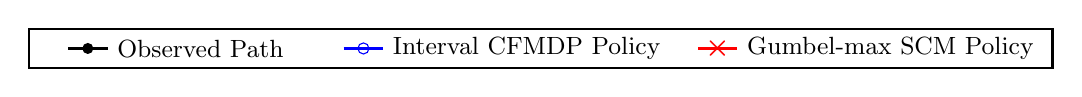
\begin{tikzpicture}[scale=1.0, every node/.style={scale=1.0}]
            \draw[thick, black] (-3, -0.25) rectangle (10, 0.25);
            %
            \draw[black, line width=1pt] (-2.5, 0.0) -- (-2,0.0);
            \fill[black] (-2.25,0.0) circle (2pt); %
            \node[right] at (-2,0.0) {\small Observed Path};
            
            %
            \draw[blue, line width=1pt] (1.0,0.0) -- (1.5,0.0);
            \node[draw=blue, circle, minimum size=4pt, inner sep=0pt] at (1.25,0.0) {}; %
            \node[right] at (1.5,0.0) {\small Interval CFMDP Policy};
            
            %
            \draw[red, line width=1pt] (5.5,0) -- (6,0);
            \node[red] at (5.75,0) {$\boldsymbol{\times}$}; %
            \node[right] at (6,0) {\small Gumbel-max SCM Policy};
        \end{tikzpicture}
    }\\
    %
    \subfigure[\footnotesize Lowest cumulative reward: Interval CFMDP ($312$), Gumbel-max SCM ($312$)]{%
        \resizebox{0.76\columnwidth}{!}{
             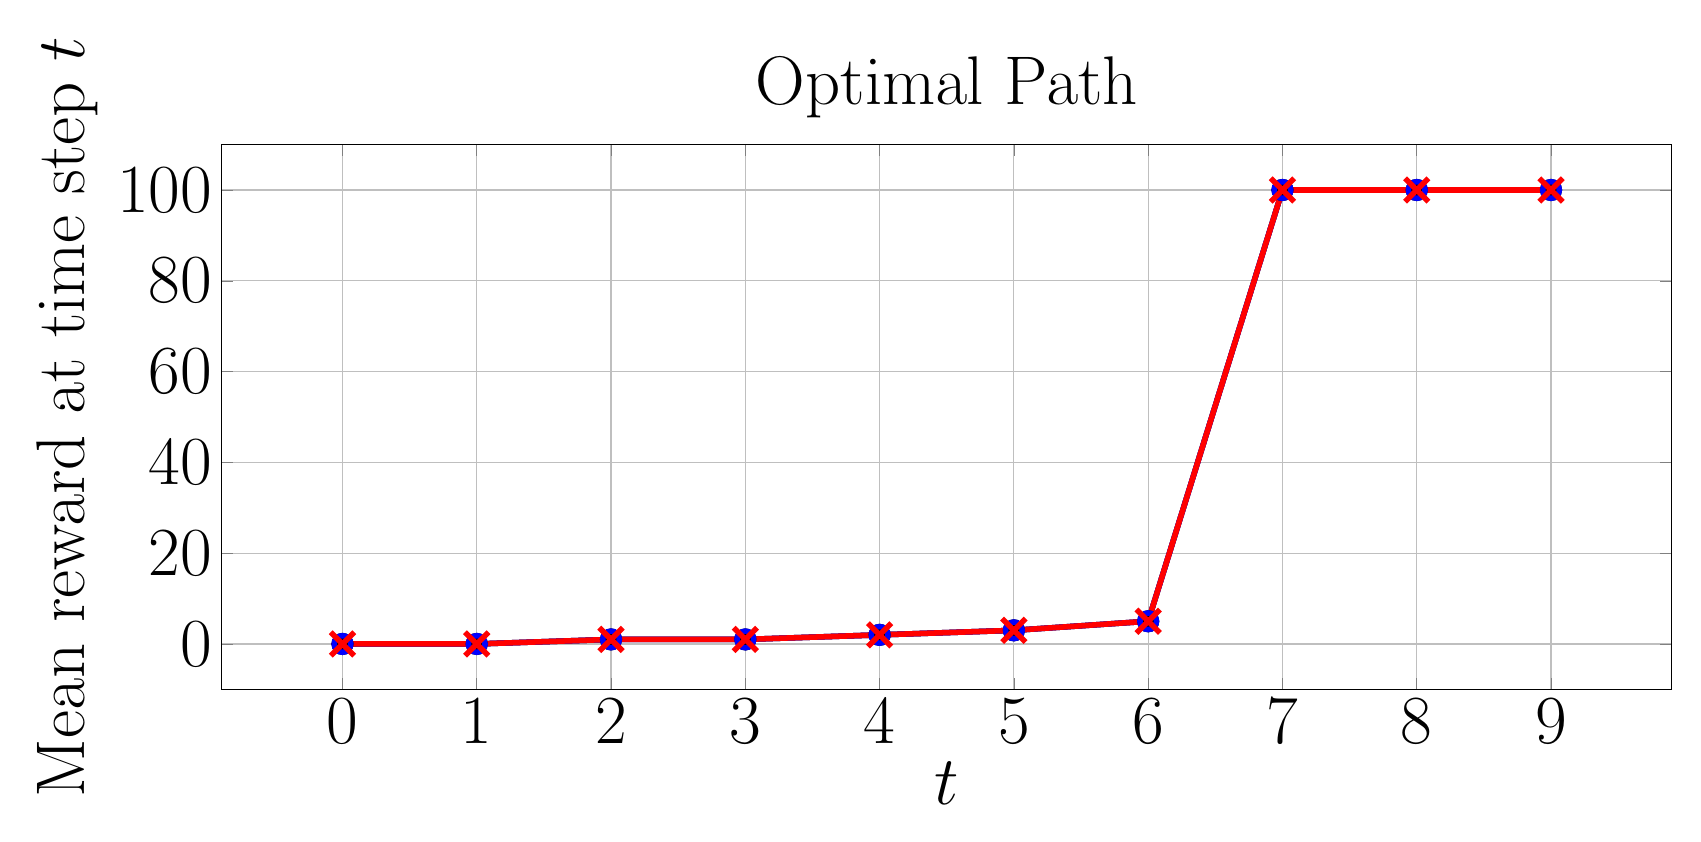
\begin{tikzpicture}
                \begin{axis}[
                    xlabel={$t$},
                    ylabel={Mean reward at time step $t$},
                    title={Optimal Path},
                    grid=both,
                    width=20cm, height=8.5cm,
                    every axis/.style={font=\Huge},
                    %
                ]
                \addplot[
                    color=black, %
                    mark=*, %
                    line width=2pt,
                    mark size=3pt,
                    error bars/.cd,
                    y dir=both, %
                    y explicit, %
                    error bar style={line width=1pt,solid},
                    error mark options={line width=1pt,mark size=4pt,rotate=90}
                ]
                coordinates {
                    (0, 0.0)  +- (0, 0.0)
                    (1, 0.0)  +- (0, 0.0) 
                    (2, 1.0)  +- (0, 0.0) 
                    (3, 1.0)  +- (0, 0.0)
                    (4, 2.0)  +- (0, 0.0)
                    (5, 3.0) +- (0, 0.0)
                    (6, 5.0) +- (0, 0.0)
                    (7, 100.0) +- (0, 0.0)
                    (8, 100.0) +- (0, 0.0)
                    (9, 100.0) +- (0, 0.0)
                };
                %
                \addplot[
                    color=blue, %
                    mark=o, %
                    line width=2pt,
                    mark size=3pt,
                    error bars/.cd,
                    y dir=both, %
                    y explicit, %
                    error bar style={line width=1pt,solid},
                    error mark options={line width=1pt,mark size=4pt,rotate=90}
                ]
                 coordinates {
                    (0, 0.0)  +- (0, 0.0)
                    (1, 0.0)  +- (0, 0.0) 
                    (2, 1.0)  +- (0, 0.0) 
                    (3, 1.0)  +- (0, 0.0)
                    (4, 2.0)  +- (0, 0.0)
                    (5, 3.0) +- (0, 0.0)
                    (6, 5.0) +- (0, 0.0)
                    (7, 100.0) +- (0, 0.0)
                    (8, 100.0) +- (0, 0.0)
                    (9, 100.0) +- (0, 0.0)
                };
                %
                \addplot[
                    color=red, %
                    mark=x, %
                    line width=2pt,
                    mark size=6pt,
                    error bars/.cd,
                    y dir=both, %
                    y explicit, %
                    error bar style={line width=1pt,solid},
                    error mark options={line width=1pt,mark size=4pt,rotate=90}
                ]
                coordinates {
                    (0, 0.0)  +- (0, 0.0)
                    (1, 0.0)  +- (0, 0.0) 
                    (2, 1.0)  +- (0, 0.0) 
                    (3, 1.0)  +- (0, 0.0)
                    (4, 2.0)  +- (0, 0.0)
                    (5, 3.0) +- (0, 0.0)
                    (6, 5.0) +- (0, 0.0)
                    (7, 100.0) +- (0, 0.0)
                    (8, 100.0) +- (0, 0.0)
                    (9, 100.0) +- (0, 0.0)
                };
                \end{axis}
            \end{tikzpicture}
         }
    }
    \hspace{1cm}
    \subfigure[\footnotesize Lowest cumulative reward: Interval CFMDP ($19$), Gumbel-max SCM ($-88$)]{%
         \resizebox{0.76\columnwidth}{!}{
            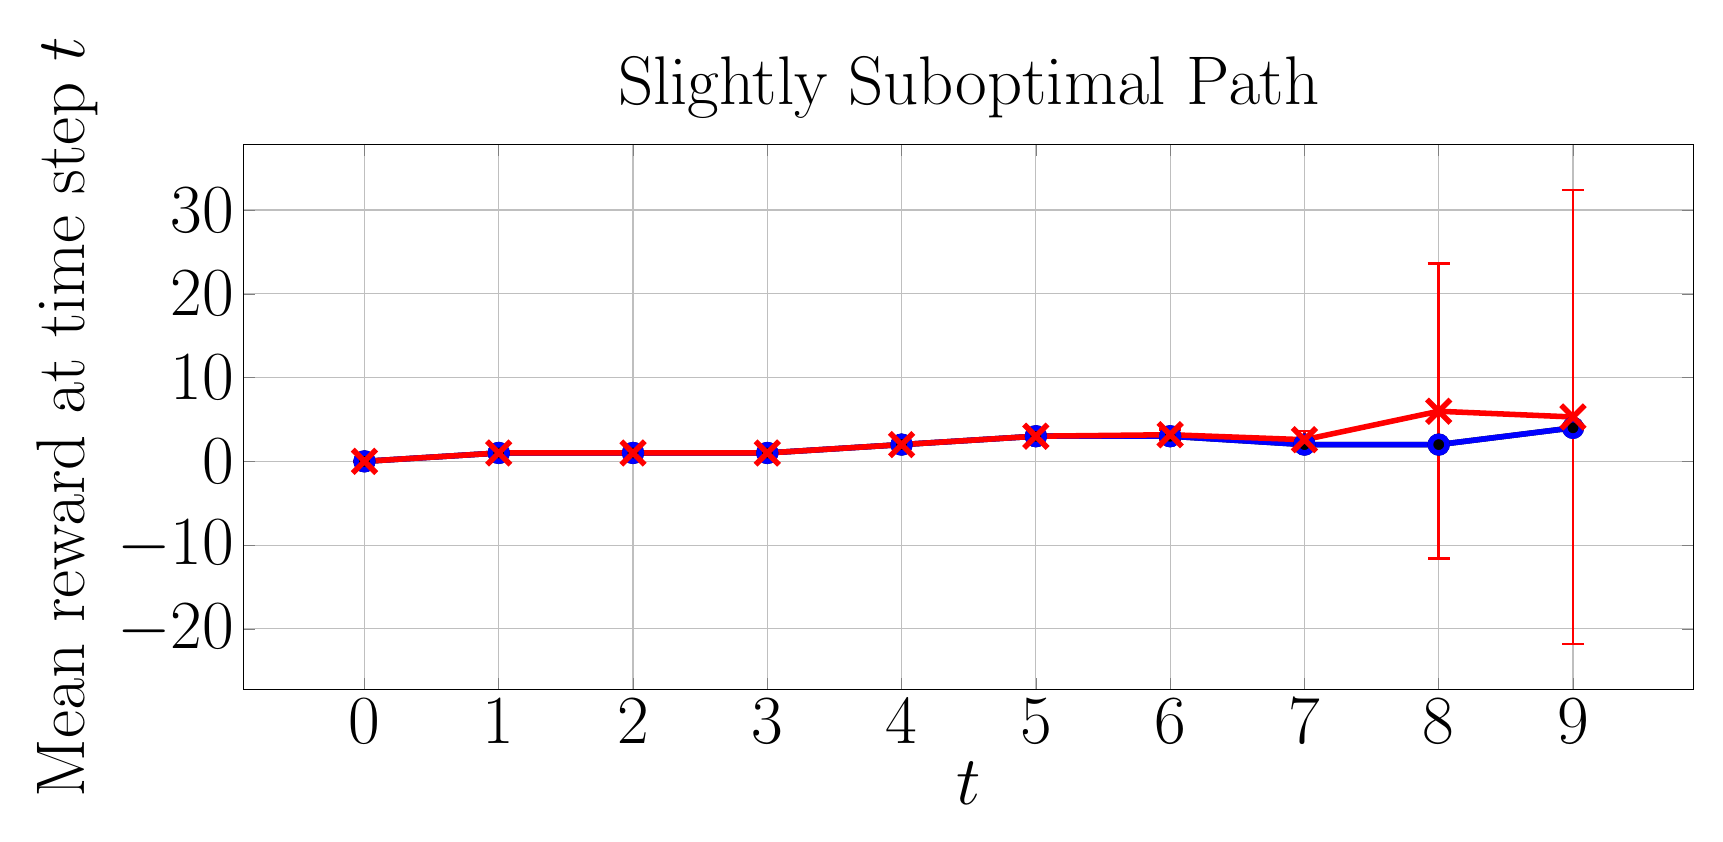
\begin{tikzpicture}
                \begin{axis}[
                    xlabel={$t$},
                    ylabel={Mean reward at time step $t$},
                    title={Slightly Suboptimal Path},
                    grid=both,
                    width=20cm, height=8.5cm,
                    every axis/.style={font=\Huge},
                    %
                ]
                \addplot[
                    color=black, %
                    mark=*, %
                    line width=2pt,
                    mark size=3pt,
                    error bars/.cd,
                    y dir=both, %
                    y explicit, %
                    error bar style={line width=1pt,solid},
                    error mark options={line width=1pt,mark size=4pt,rotate=90}
                ]
              coordinates {
                    (0, 0.0)  +- (0, 0.0)
                    (1, 1.0)  +- (0, 0.0) 
                    (2, 1.0)  +- (0, 0.0) 
                    (3, 1.0)  +- (0, 0.0)
                    (4, 2.0)  +- (0, 0.0)
                    (5, 3.0) +- (0, 0.0)
                    (6, 3.0) +- (0, 0.0)
                    (7, 2.0) +- (0, 0.0)
                    (8, 2.0) +- (0, 0.0)
                    (9, 4.0) +- (0, 0.0)
                };
                %
                \addplot[
                    color=blue, %
                    mark=o, %
                    line width=2pt,
                    mark size=3pt,
                    error bars/.cd,
                    y dir=both, %
                    y explicit, %
                    error bar style={line width=1pt,solid},
                    error mark options={line width=1pt,mark size=4pt,rotate=90}
                ]
              coordinates {
                    (0, 0.0)  +- (0, 0.0)
                    (1, 1.0)  +- (0, 0.0) 
                    (2, 1.0)  +- (0, 0.0) 
                    (3, 1.0)  +- (0, 0.0)
                    (4, 2.0)  +- (0, 0.0)
                    (5, 3.0) +- (0, 0.0)
                    (6, 3.0) +- (0, 0.0)
                    (7, 2.0) +- (0, 0.0)
                    (8, 2.0) +- (0, 0.0)
                    (9, 4.0) +- (0, 0.0)
                };
                %
                \addplot[
                    color=red, %
                    mark=x, %
                    line width=2pt,
                    mark size=6pt,
                    error bars/.cd,
                    y dir=both, %
                    y explicit, %
                    error bar style={line width=1pt,solid},
                    error mark options={line width=1pt,mark size=4pt,rotate=90}
                ]
                coordinates {
                    (0, 0.0)  +- (0, 0.0)
                    (1, 1.0)  +- (0, 0.0) 
                    (2, 1.0)  +- (0, 0.0) 
                    (3, 1.0)  +- (0, 0.0)
                    (4, 2.0)  += (0, 0.0)
                    (5, 3.0)  += (0, 0.0)
                    (6, 3.17847) += (0, 0.62606746) -= (0, 0.62606746)
                    (7, 2.5832885) += (0, 1.04598233) -= (0, 1.04598233)
                    (8, 5.978909) += (0, 17.60137623) -= (0, 17.60137623)
                    (9, 5.297059) += (0, 27.09227512) -= (0, 27.09227512)
                };
                \end{axis}
            \end{tikzpicture}
         }
    }\\[-1.5pt]
    \subfigure[\footnotesize Lowest cumulative reward: Interval CFMDP ($14$), Gumbel-max SCM ($-598$)]{%
         \resizebox{0.76\columnwidth}{!}{
             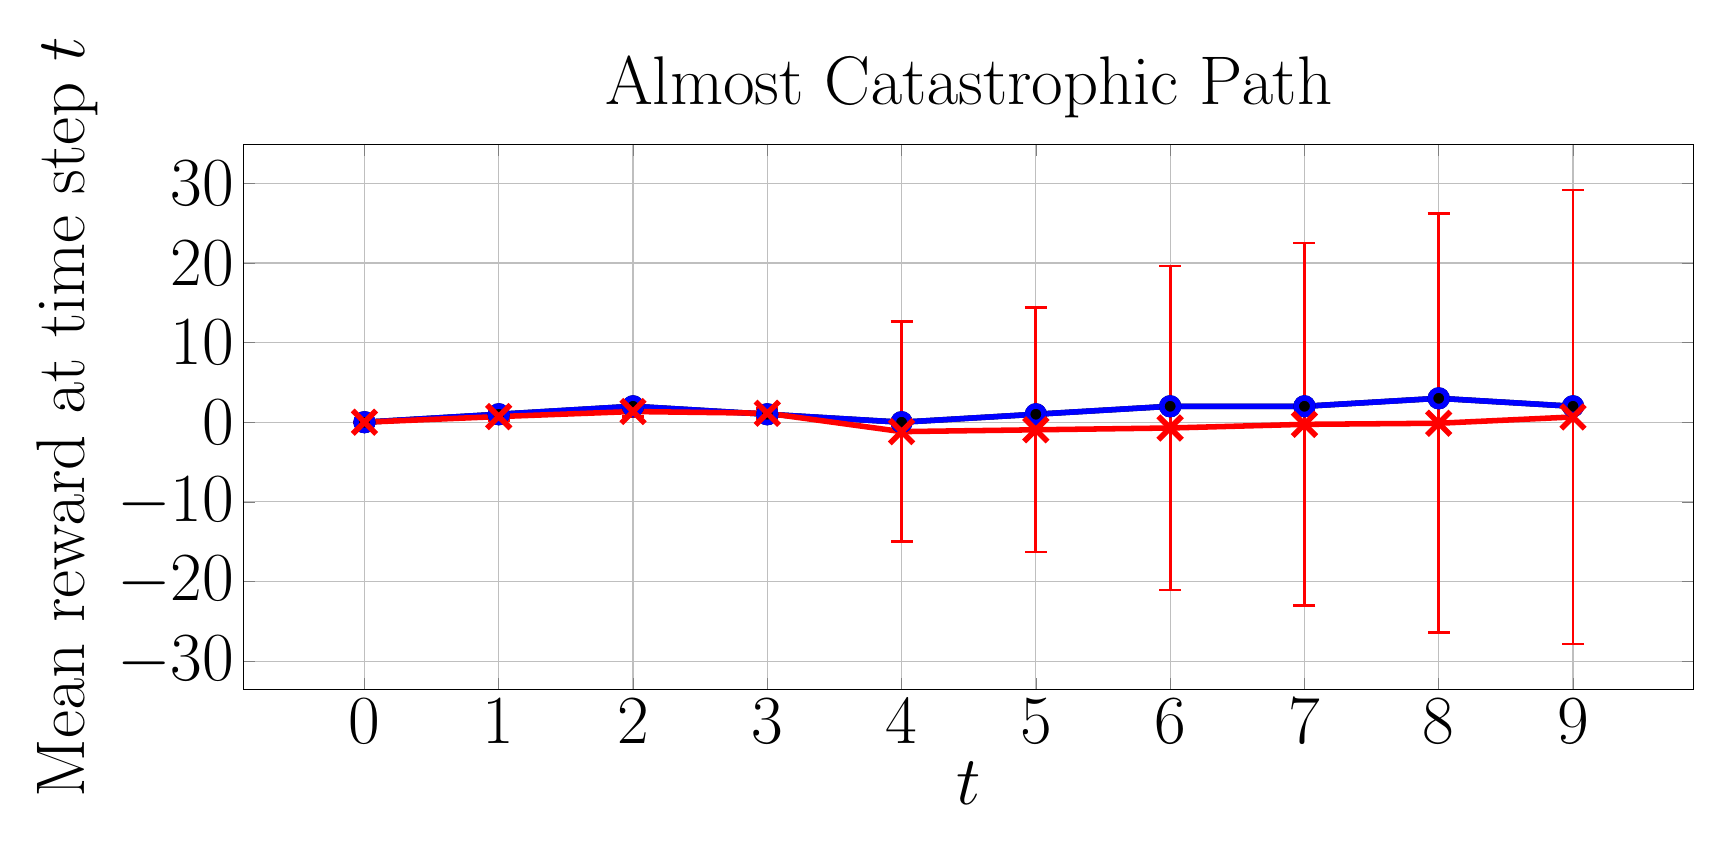
\begin{tikzpicture}
                \begin{axis}[
                    xlabel={$t$},
                    ylabel={Mean reward at time step $t$},
                    title={Almost Catastrophic Path},
                    grid=both,
                    width=20cm, height=8.5cm,
                    every axis/.style={font=\Huge},
                    %
                ]
                \addplot[
                    color=black, %
                    mark=*, %
                    line width=2pt,
                    mark size=3pt,
                    error bars/.cd,
                    y dir=both, %
                    y explicit, %
                    error bar style={line width=1pt,solid},
                    error mark options={line width=1pt,mark size=4pt,rotate=90}
                ]
                coordinates {
                    (0, 0.0)  +- (0, 0.0)
                    (1, 1.0)  +- (0, 0.0) 
                    (2, 2.0)  +- (0, 0.0) 
                    (3, 1.0)  +- (0, 0.0)
                    (4, 0.0)  +- (0, 0.0)
                    (5, 1.0) +- (0, 0.0)
                    (6, 2.0) +- (0, 0.0)
                    (7, 2.0) +- (0, 0.0)
                    (8, 3.0) +- (0, 0.0)
                    (9, 2.0) +- (0, 0.0)
                };
                %
                \addplot[
                    color=blue, %
                    mark=o, %
                    line width=2pt,
                    mark size=3pt,
                    error bars/.cd,
                    y dir=both, %
                    y explicit, %
                    error bar style={line width=1pt,solid},
                    error mark options={line width=1pt,mark size=4pt,rotate=90}
                ]
                coordinates {
                    (0, 0.0)  +- (0, 0.0)
                    (1, 1.0)  +- (0, 0.0) 
                    (2, 2.0)  +- (0, 0.0) 
                    (3, 1.0)  +- (0, 0.0)
                    (4, 0.0)  +- (0, 0.0)
                    (5, 1.0) +- (0, 0.0)
                    (6, 2.0) +- (0, 0.0)
                    (7, 2.0) +- (0, 0.0)
                    (8, 3.0) +- (0, 0.0)
                    (9, 2.0) +- (0, 0.0)
                };
                %
                \addplot[
                    color=red, %
                    mark=x, %
                    line width=2pt,
                    mark size=6pt,
                    error bars/.cd,
                    y dir=both, %
                    y explicit, %
                    error bar style={line width=1pt,solid},
                    error mark options={line width=1pt,mark size=4pt,rotate=90}
                ]
                coordinates {
                    (0, 0.0)  +- (0, 0.0)
                    (1, 0.7065655)  +- (0, 0.4553358) 
                    (2, 1.341673)  +- (0, 0.67091621) 
                    (3, 1.122926)  +- (0, 0.61281824)
                    (4, -1.1821935)  +- (0, 13.82444042)
                    (5, -0.952399)  +- (0, 15.35195457)
                    (6, -0.72672) +- (0, 20.33508414)
                    (7, -0.268983) +- (0, 22.77861454)
                    (8, -0.1310835) +- (0, 26.31013314)
                    (9, 0.65806) +- (0, 28.50670214)
                };
                %
            %
            %
            %
            %
            %
            %
            %
            %
            %
            %
            %
            %
            %
            %
            %
            %
            %
            %
                \end{axis}
            \end{tikzpicture}
         }
    }
    \hspace{1cm}
    \subfigure[\footnotesize Lowest cumulative reward: Interval CFMDP ($-698$), Gumbel-max SCM ($-698$)]{%
         \resizebox{0.76\columnwidth}{!}{
            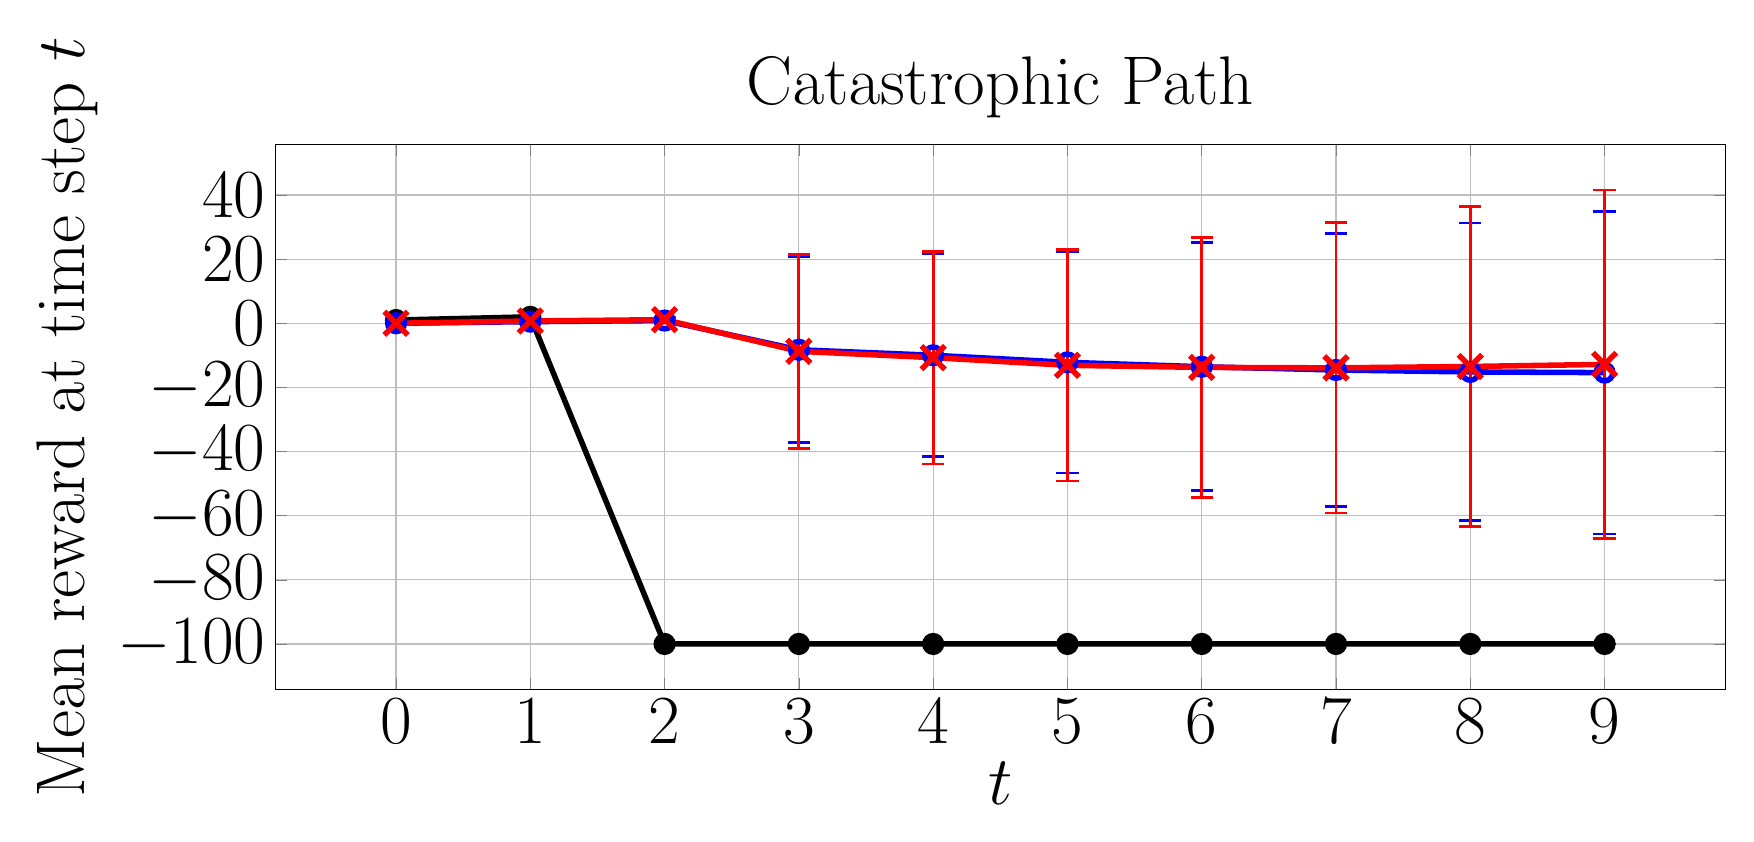
\begin{tikzpicture}
                \begin{axis}[
                    xlabel={$t$},
                    ylabel={Mean reward at time step $t$},
                    title={Catastrophic Path},
                    grid=both,
                    width=20cm, height=8.5cm,
                    every axis/.style={font=\Huge},
                    %
                ]
                \addplot[
                    color=black, %
                    mark=*, %
                    line width=2pt,
                    mark size=3pt,
                    error bars/.cd,
                    y dir=both, %
                    y explicit, %
                    error bar style={line width=1pt,solid},
                    error mark options={line width=1pt,mark size=4pt,rotate=90}
                ]
                coordinates {
                    (0, 1.0)  +- (0, 0.0)
                    (1, 2.0)  +- (0, 0.0) 
                    (2, -100.0)  +- (0, 0.0) 
                    (3, -100.0)  +- (0, 0.0)
                    (4, -100.0)  +- (0, 0.0)
                    (5, -100.0) +- (0, 0.0)
                    (6, -100.0) +- (0, 0.0)
                    (7, -100.0) +- (0, 0.0)
                    (8, -100.0) +- (0, 0.0)
                    (9, -100.0) +- (0, 0.0)
                };
                %
                \addplot[
                    color=blue, %
                    mark=o, %
                    line width=2pt,
                    mark size=3pt,
                    error bars/.cd,
                    y dir=both, %
                    y explicit, %
                    error bar style={line width=1pt,solid},
                    error mark options={line width=1pt,mark size=4pt,rotate=90}
                ]
                coordinates {
                    (0, 0.0)  +- (0, 0.0)
                    (1, 0.504814)  +- (0, 0.49997682) 
                    (2, 0.8439835)  +- (0, 0.76831917) 
                    (3, -8.2709165)  +- (0, 28.93656754)
                    (4, -9.981082)  +- (0, 31.66825363)
                    (5, -12.1776325) +- (0, 34.53463233)
                    (6, -13.556076) +- (0, 38.62845372)
                    (7, -14.574418) +- (0, 42.49603359)
                    (8, -15.1757075) +- (0, 46.41913968)
                    (9, -15.3900395) +- (0, 50.33563368)
                };
                %
                \addplot[
                    color=red, %
                    mark=x, %
                    line width=2pt,
                    mark size=6pt,
                    error bars/.cd,
                    y dir=both, %
                    y explicit, %
                    error bar style={line width=1pt,solid},
                    error mark options={line width=1pt,mark size=4pt,rotate=90}
                ]
                coordinates {
                    (0, 0.0)  +- (0, 0.0)
                    (1, 0.701873)  +- (0, 0.45743556) 
                    (2, 1.1227805)  +- (0, 0.73433129) 
                    (3, -8.7503255)  +- (0, 30.30257976)
                    (4, -10.722092)  +- (0, 33.17618589)
                    (5, -13.10721)  +- (0, 36.0648089)
                    (6, -13.7631645) +- (0, 40.56553451)
                    (7, -13.909043) +- (0, 45.23829402)
                    (8, -13.472517) +- (0, 49.96270296)
                    (9, -12.8278835) +- (0, 54.38618735)
                };
                %
            %
            %
            %
            %
            %
            %
            %
            %
            %
            %
            %
            %
            %
            %
            %
            %
            %
            %
                \end{axis}
            \end{tikzpicture}
         }
    }
    \caption{Average instant reward of CF paths induced by policies on GridWorld $p=0.4$.}
    \label{fig: reward p=0.4}
\end{figure*}

\subsection{Experimental Setup}
To compare policy performance, we measure the average rewards of counterfactual paths induced by our policy and the Gumbel-max policy by uniformly sampling $200$ counterfactual MDPs from the ICFMDP and generating $10,000$ counterfactual paths over each sampled CFMDP. \jl{Since the interval CFMDP depends on the observed path, we select $4$  paths of varying optimality to evaluate how the observed path impacts the performance of both policies: an optimal path, a slightly suboptimal path that could reach the optimal reward with a few changes, a catastrophic path that enters a catastrophic, terminal state with low reward, and an almost catastrophic path that was close to entering a catastrophic state.} When measuring the average probability bound widths and execution time needed to generate the ICFMDPs, we averaged over $20$ randomly generated observed paths
\footnote{Further training details are provided in Appendix \ref{app: training details}, and the code is provided at \href{https://github.com/ddv-lab/robust-cf-inference-in-MDPs}{https://github.com/ddv-lab/robust-cf-inference-in-MDPs}
%
%
.}.

\subsection{GridWorld}
\jl{The GridWorld MDP is a $4 \times 4$ grid where an agent must navigate from the top-left corner to the goal state in the bottom-right corner, avoiding a dangerous terminal state in the centre. At each time step, the agent can move up, down, left, or right, but there is a small probability (controlled by hyper-parameter $p$) of moving in an unintended direction. As the agent nears the goal, the reward for each state increases, culminating in a reward of $+100$ for reaching the goal. Entering the dangerous state results in a penalty of $-100$. We use two versions of GridWorld: a less stochastic version with $p=0.9$ (i.e., $90$\% chance of moving in the chosen direction) and a more stochastic version with $p=0.4$.}

\paragraph{GridWorld ($p=0.9$)}
When $p=0.9$, the counterfactual probability bounds are typically narrow (see Table \ref{tab:nonzero_probs} for average measurements). Consequently, as shown in Figure \ref{fig: reward p=0.9}, both policies are nearly identical and perform similarly well across the optimal, slightly suboptimal, and catastrophic paths.
%
However, for the almost catastrophic path, the interval CFMDP path is more conservative and follows the observed path more closely (as this is where the probability bounds are narrowest), which typically requires one additional step to reach the goal state than the Gumbel-max SCM policy.
%

\paragraph{GridWorld ($p=0.4$)}
\jl{When $p=0.4$, the GridWorld environment becomes more uncertain, increasing the risk of entering the dangerous state even if correct actions are chosen. Thus, as shown in Figure \ref{fig: reward p=0.4}, the interval CFMDP policy adopts a more conservative approach, avoiding deviation from the observed policy if it cannot guarantee higher counterfactual rewards (see the slightly suboptimal and almost catastrophic paths), whereas the Gumbel-max SCM is inconsistent: it can yield higher rewards, but also much lower rewards, reflected in the wide error bars.} For the catastrophic path, both policies must deviate from the observed path to achieve a higher reward and, in this case, perform similarly.
%
%
%
%
\subsection{Sepsis}
The Sepsis MDP \citep{oberst2019counterfactual} simulates trajectories of Sepsis patients. Each state consists of four vital signs (heart rate, blood pressure, oxygen concentration, and glucose levels), categorised as low, normal, or high.
and three treatments that can be toggled on/off at each time step (8 actions in total). Unlike \citet{oberst2019counterfactual}, we scale rewards based on the number of out-of-range vital signs, between $-1000$ (patient dies) and $1000$ (patient discharged). \jl{Like the GridWorld $p=0.4$ experiment, the Sepsis MDP is highly uncertain, as many states are equally likely to lead to optimal and poor outcomes. Thus, as shown in Figure \ref{fig: reward sepsis}, both policies follow the observed optimal and almost catastrophic paths to guarantee rewards are no worse than the observation.} However, improving the catastrophic path requires deviating from the observation. Here, the Gumbel-max SCM policy, on average, performs better than the interval CFMDP policy. But, since both policies have lower bounds clipped at $-1000$, neither policy reliably improves over the observation. In contrast, for the slightly suboptimal path, the interval CFMDP policy performs significantly better, shown by its higher lower bounds. 
Moreover, in these two cases, the worst-case counterfactual path generated by the interval CFMDP policy is better than that of the Gumbel-max SCM policy,
indicating its greater robustness.
%
\begin{figure*}
    \centering
     \resizebox{0.6\textwidth}{!}{
        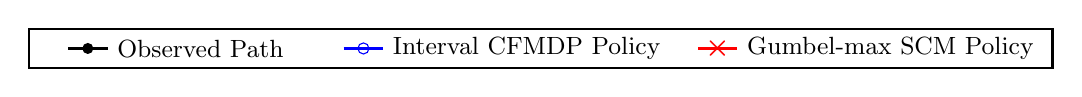
\begin{tikzpicture}[scale=1.0, every node/.style={scale=1.0}]
            \draw[thick, black] (-3, -0.25) rectangle (10, 0.25);
            %
            \draw[black, line width=1pt] (-2.5, 0.0) -- (-2,0.0);
            \fill[black] (-2.25,0.0) circle (2pt); %
            \node[right] at (-2,0.0) {\small Observed Path};
            
            %
            \draw[blue, line width=1pt] (1.0,0.0) -- (1.5,0.0);
            \node[draw=blue, circle, minimum size=4pt, inner sep=0pt] at (1.25,0.0) {}; %
            \node[right] at (1.5,0.0) {\small Interval CFMDP Policy};
            
            %
            \draw[red, line width=1pt] (5.5,0) -- (6,0);
            \node[red] at (5.75,0) {$\boldsymbol{\times}$}; %
            \node[right] at (6,0) {\small Gumbel-max SCM Policy};
        \end{tikzpicture}
    }\\
    \subfigure[\footnotesize Lowest cumulative reward: Interval CFMDP ($8000$), Gumbel-max SCM ($8000$)]{%
         \resizebox{0.76\columnwidth}{!}{
             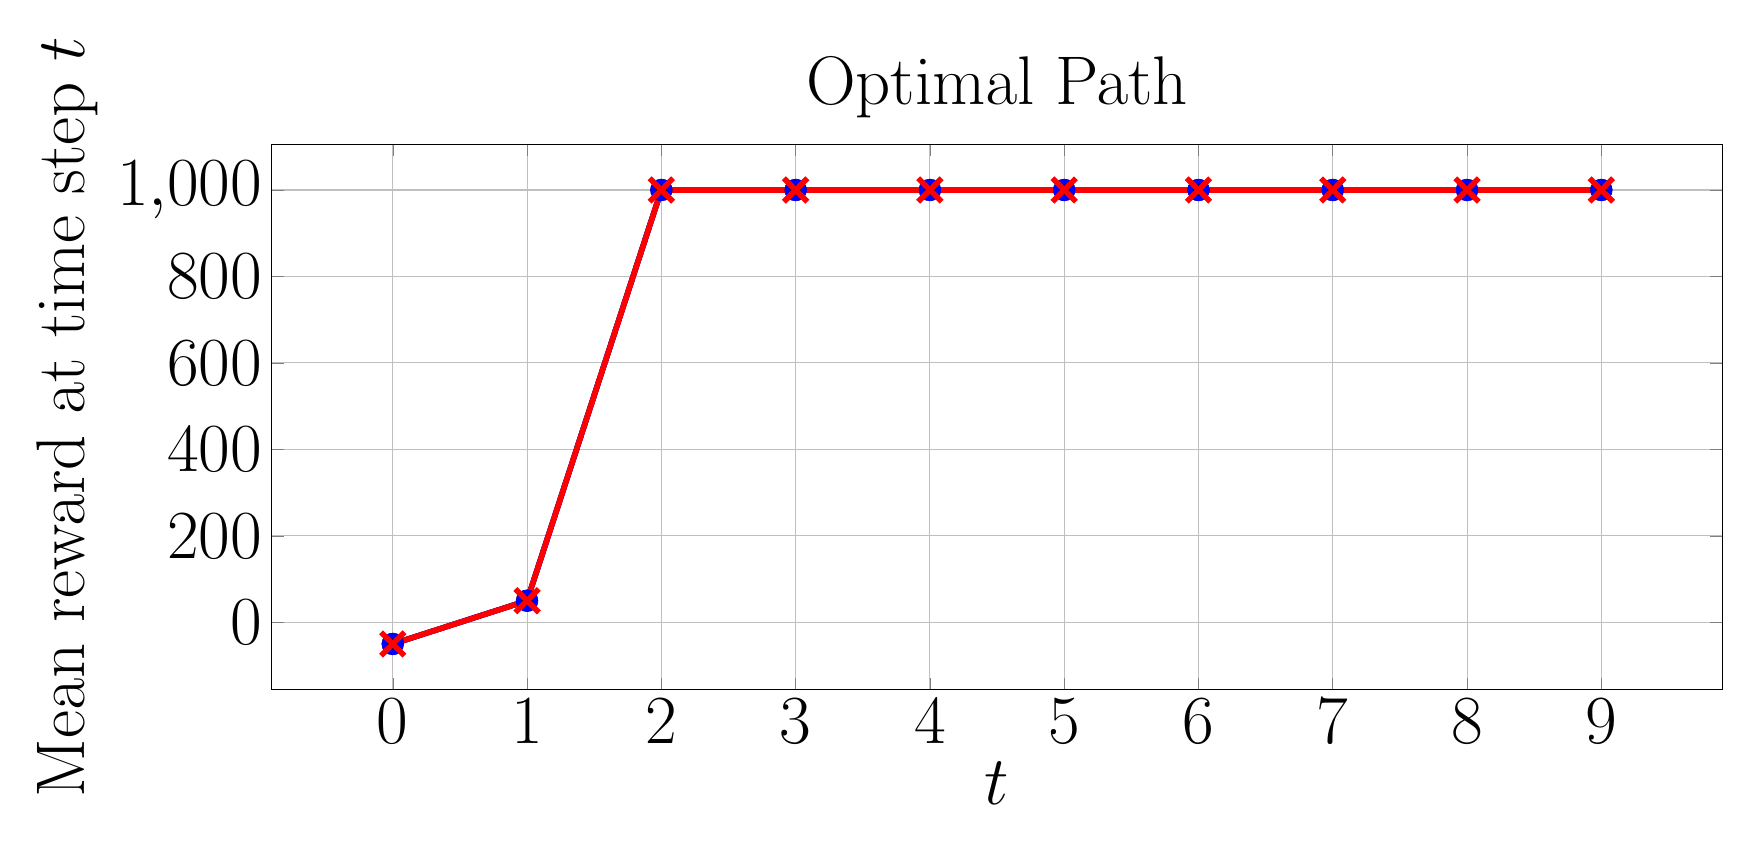
\begin{tikzpicture}
                \begin{axis}[
                    xlabel={$t$},
                    ylabel={Mean reward at time step $t$},
                    title={Optimal Path},
                    grid=both,
                    width=20cm, height=8.5cm,
                    every axis/.style={font=\Huge},
                    %
                ]
                \addplot[
                    color=black, %
                    mark=*, %
                    line width=2pt,
                    mark size=3pt,
                ]
                coordinates {
                    (0, -50.0)
                    (1, 50.0)
                    (2, 1000.0)
                    (3, 1000.0)
                    (4, 1000.0)
                    (5, 1000.0)
                    (6, 1000.0)
                    (7, 1000.0)
                    (8, 1000.0)
                    (9, 1000.0)
                };
                %
                \addplot[
                    color=blue, %
                    mark=o, %
                    line width=2pt,
                    mark size=3pt,
                    error bars/.cd,
                    y dir=both, %
                    y explicit, %
                    error bar style={line width=1pt,solid},
                    error mark options={line width=1pt,mark size=4pt,rotate=90}
                ]
                coordinates {
                    (0, -50.0)  +- (0, 0.0)
                    (1, 50.0)  +- (0, 0.0) 
                    (2, 1000.0)  +- (0, 0.0) 
                    (3, 1000.0)  +- (0, 0.0)
                    (4, 1000.0)  +- (0, 0.0)
                    (5, 1000.0) +- (0, 0.0)
                    (6, 1000.0) +- (0, 0.0)
                    (7, 1000.0) +- (0, 0.0)
                    (8, 1000.0) +- (0, 0.0)
                    (9, 1000.0) +- (0, 0.0)
                };
                %
                \addplot[
                    color=red, %
                    mark=x, %
                    line width=2pt,
                    mark size=6pt,
                    error bars/.cd,
                    y dir=both, %
                    y explicit, %
                    error bar style={line width=1pt,solid},
                    error mark options={line width=1pt,mark size=4pt,rotate=90}
                ]
                coordinates {
                    (0, -50.0)  +- (0, 0.0)
                    (1, 50.0)  +- (0, 0.0) 
                    (2, 1000.0)  +- (0, 0.0) 
                    (3, 1000.0)  +- (0, 0.0)
                    (4, 1000.0)  +- (0, 0.0)
                    (5, 1000.0) +- (0, 0.0)
                    (6, 1000.0) +- (0, 0.0)
                    (7, 1000.0) +- (0, 0.0)
                    (8, 1000.0) +- (0, 0.0)
                    (9, 1000.0) +- (0, 0.0)
                };
                %
                \end{axis}
            \end{tikzpicture}
         }
    }
    \hspace{1cm}
    \subfigure[\footnotesize Lowest cumulative reward: Interval CFMDP ($-5980$), Gumbel-max SCM ($-8000$)]{%
         \resizebox{0.76\columnwidth}{!}{
            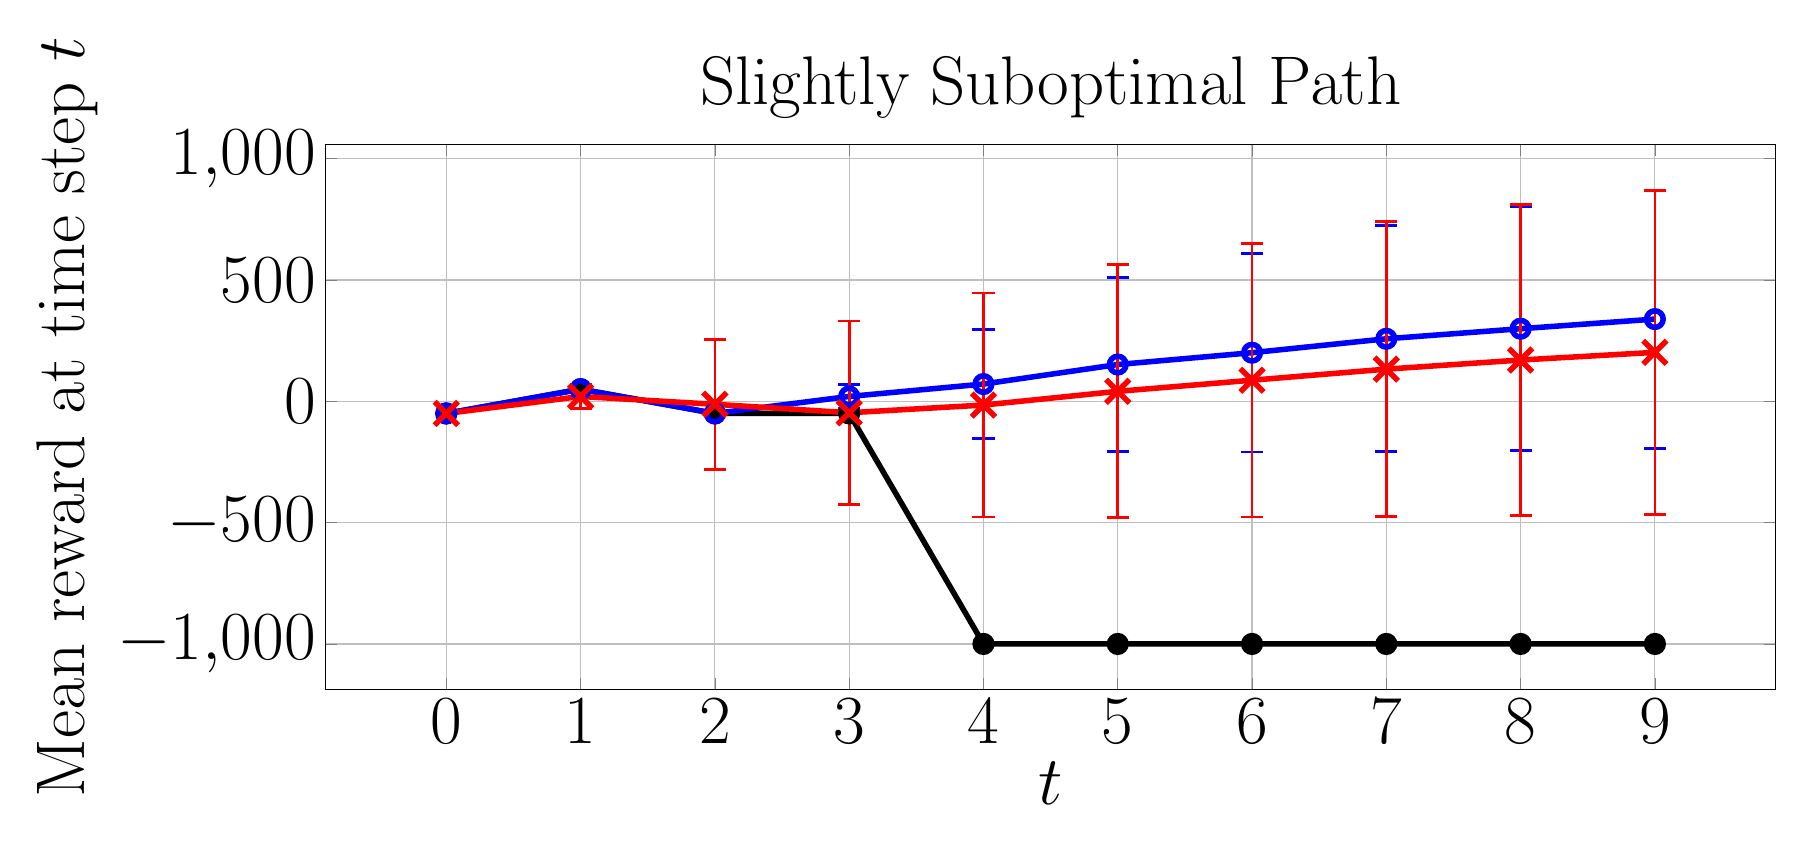
\begin{tikzpicture}
                \begin{axis}[
                    xlabel={$t$},
                    ylabel={Mean reward at time step $t$},
                    title={Slightly Suboptimal Path},
                    grid=both,
                    width=20cm, height=8.5cm,
                    every axis/.style={font=\Huge},
                    %
                ]
               \addplot[
                    color=black, %
                    mark=*, %
                    line width=2pt,
                    mark size=3pt,
                ]
                coordinates {
                    (0, -50.0)
                    (1, 50.0)
                    (2, -50.0)
                    (3, -50.0)
                    (4, -1000.0)
                    (5, -1000.0)
                    (6, -1000.0)
                    (7, -1000.0)
                    (8, -1000.0)
                    (9, -1000.0)
                };
                %
                \addplot[
                    color=blue, %
                    mark=o, %
                    line width=2pt,
                    mark size=3pt,
                    error bars/.cd,
                    y dir=both, %
                    y explicit, %
                    error bar style={line width=1pt,solid},
                    error mark options={line width=1pt,mark size=4pt,rotate=90}
                ]
                coordinates {
                    (0, -50.0)  +- (0, 0.0)
                    (1, 50.0)  +- (0, 0.0) 
                    (2, -50.0)  +- (0, 0.0) 
                    (3, 20.0631)  +- (0, 49.97539413)
                    (4, 71.206585)  +- (0, 226.02033693)
                    (5, 151.60797) +- (0, 359.23292559)
                    (6, 200.40593) +- (0, 408.86185176)
                    (7, 257.77948) +- (0, 466.10372804)
                    (8, 299.237465) +- (0, 501.82579506)
                    (9, 338.9129) +- (0, 532.06124996)
                };
                %
                \addplot[
                    color=red, %
                    mark=x, %
                    line width=2pt,
                    mark size=6pt,
                    error bars/.cd,
                    y dir=both, %
                    y explicit, %
                    error bar style={line width=1pt,solid},
                    error mark options={line width=1pt,mark size=4pt,rotate=90}
                ]
                coordinates {
                    (0, -50.0)  +- (0, 0.0)
                    (1, 20.00736)  +- (0, 49.99786741) 
                    (2, -12.282865)  +- (0, 267.598755) 
                    (3, -47.125995)  +- (0, 378.41755832)
                    (4, -15.381965)  +- (0, 461.77616558)
                    (5, 41.15459) +- (0, 521.53189262)
                    (6, 87.01595) +- (0, 564.22243126 )
                    (7, 132.62376) +- (0, 607.31338037)
                    (8, 170.168145) +- (0, 641.48013693)
                    (9, 201.813135) +- (0, 667.29441777)
                };
                %
                %
                %
                %
                %
                %
                %
                %
                %
                %
                %
                %
                %
                %
                %
                %
                %
                %
                %
                \end{axis}
            \end{tikzpicture}
         }
    }\\[-1.5pt]
    \subfigure[\footnotesize Lowest cumulative reward: Interval CFMDP ($100$), Gumbel-max SCM ($100$)]{%
         \resizebox{0.76\columnwidth}{!}{
             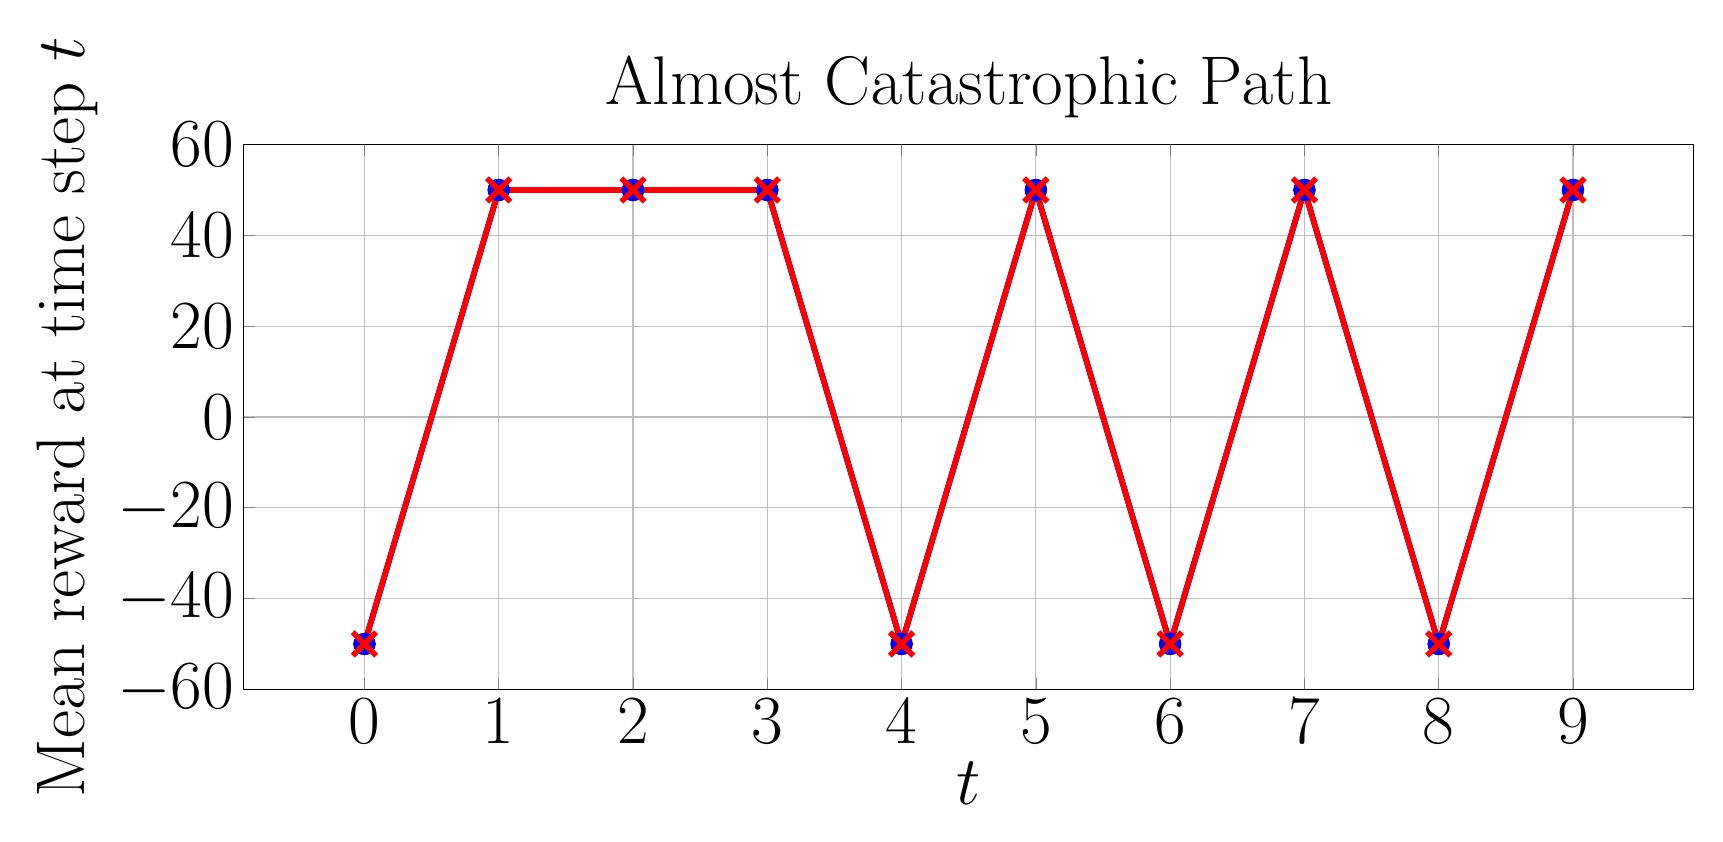
\begin{tikzpicture}
                \begin{axis}[
                    xlabel={$t$},
                    ylabel={Mean reward at time step $t$},
                    title={Almost Catastrophic Path},
                    grid=both,
                    every axis/.style={font=\Huge},
                    width=20cm, height=8.5cm,
                    %
                ]
               \addplot[
                    color=black, %
                    mark=*, %
                    line width=2pt,
                    mark size=3pt,
                ]
                coordinates {
                    (0, -50.0)
                    (1, 50.0)
                    (2, 50.0)
                    (3, 50.0)
                    (4, -50.0)
                    (5, 50.0)
                    (6, -50.0)
                    (7, 50.0)
                    (8, -50.0)
                    (9, 50.0)
                };
                %
                %
                \addplot[
                    color=blue, %
                    mark=o, %
                    line width=2pt,
                    mark size=3pt,
                    error bars/.cd,
                    y dir=both, %
                    y explicit, %
                    error bar style={line width=1pt,solid},
                    error mark options={line width=1pt,mark size=4pt,rotate=90}
                ]
                coordinates {
                    (0, -50.0)  +- (0, 0.0)
                    (1, 50.0)  +- (0, 0.0) 
                    (2, 50.0)  +- (0, 0.0) 
                    (3, 50.0)  +- (0, 0.0)
                    (4, -50.0)  +- (0, 0.0)
                    (5, 50.0) +- (0, 0.0)
                    (6, -50.0) +- (0, 0.0)
                    (7, 50.0) +- (0, 0.0)
                    (8, -50.0) +- (0, 0.0)
                    (9, 50.0) +- (0, 0.0)
                };
                %
                \addplot[
                    color=red, %
                    mark=x, %
                    line width=2pt,
                    mark size=6pt,
                    error bars/.cd,
                    y dir=both, %
                    y explicit, %
                    error bar style={line width=1pt,solid},
                    error mark options={line width=1pt,mark size=4pt,rotate=90}
                ]
                coordinates {
                    (0, -50.0)  +- (0, 0.0)
                    (1, 50.0)  +- (0, 0.0) 
                    (2, 50.0)  +- (0, 0.0) 
                    (3, 50.0)  +- (0, 0.0)
                    (4, -50.0)  +- (0, 0.0)
                    (5, 50.0) +- (0, 0.0)
                    (6, -50.0) +- (0, 0.0)
                    (7, 50.0) +- (0, 0.0)
                    (8, -50.0) +- (0, 0.0)
                    (9, 50.0) +- (0, 0.0)
                };
                %
                %
                %
                %
                %
                %
                %
                %
                %
                %
                %
                %
                %
                %
                %
                %
                %
                %
                %
                \end{axis}
            \end{tikzpicture}
         }
    }
    \hspace{1cm}
    \subfigure[\footnotesize Lowest cumulative reward: Interval CFMDP ($-7150$), Gumbel-max SCM ($-9050$)]{%
         \resizebox{0.76\columnwidth}{!}{
            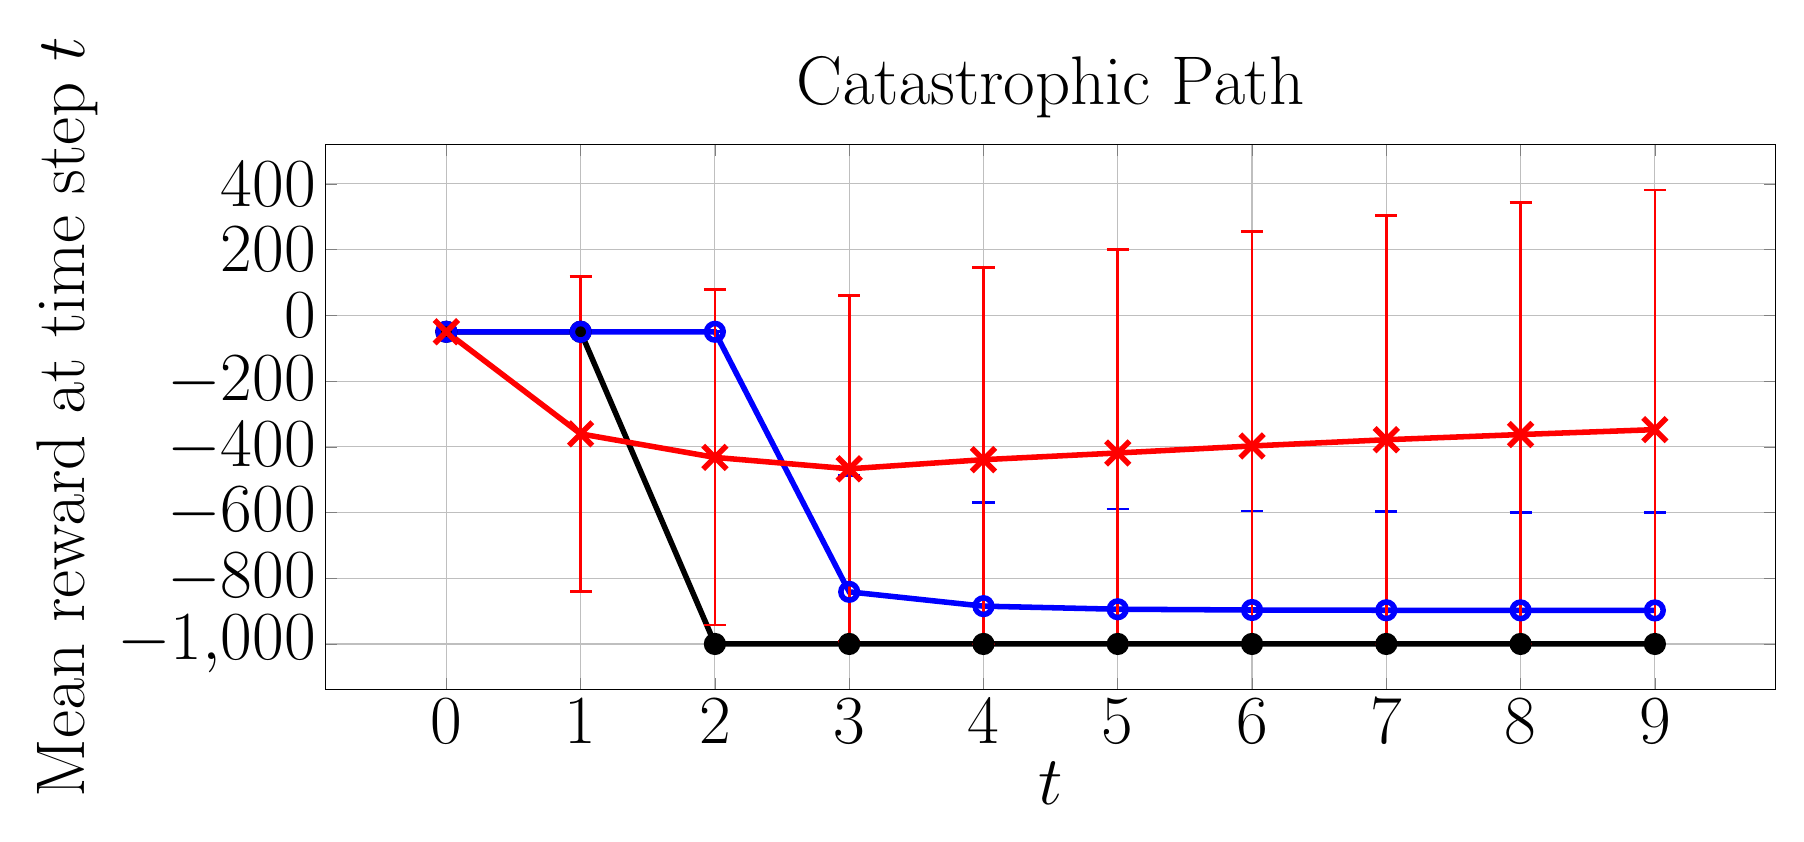
\begin{tikzpicture}
                \begin{axis}[
                    xlabel={$t$},
                    ylabel={Mean reward at time step $t$},
                    title={Catastrophic Path},
                    grid=both,
                    width=20cm, height=8.5cm,
                    every axis/.style={font=\Huge},
                    %
                ]
               \addplot[
                    color=black, %
                    mark=*, %
                    line width=2pt,
                    mark size=3pt,
                ]
                coordinates {
                    (0, -50.0)
                    (1, -50.0)
                    (2, -1000.0)
                    (3, -1000.0)
                    (4, -1000.0)
                    (5, -1000.0)
                    (6, -1000.0)
                    (7, -1000.0)
                    (8, -1000.0)
                    (9, -1000.0)
                };
                %
                %
                \addplot[
                    color=blue, %
                    mark=o, %
                    line width=2pt,
                    mark size=3pt,
                    error bars/.cd,
                    y dir=both, %
                    y explicit, %
                    error bar style={line width=1pt,solid},
                    error mark options={line width=1pt,mark size=4pt,rotate=90}
                ]
                coordinates {
                    (0, -50.0)  +- (0, 0.0)
                    (1, -50.0)  +- (0, 0.0) 
                    (2, -50.0)  +- (0, 0.0) 
                    (3, -841.440725)  += (0, 354.24605512) -= (0, 158.559275)
                    (4, -884.98225)  += (0, 315.37519669) -= (0, 115.01775)
                    (5, -894.330425) += (0, 304.88572805) -= (0, 105.669575)
                    (6, -896.696175) += (0, 301.19954514) -= (0, 103.303825)
                    (7, -897.4635) += (0, 299.61791279) -= (0, 102.5365)
                    (8, -897.77595) += (0, 298.80392585) -= (0, 102.22405)
                    (9, -897.942975) += (0, 298.32920557) -= (0, 102.057025)
                };
                %
                \addplot[
                    color=red, %
                    mark=x, %
                    line width=2pt,
                    mark size=6pt,
                    error bars/.cd,
                    y dir=both, %
                    y explicit, %
                    error bar style={line width=1pt,solid},
                    error mark options={line width=1pt,mark size=4pt,rotate=90}
                ]
            coordinates {
                    (0, -50.0)  +- (0, 0.0)
                    (1, -360.675265)  +- (0, 479.39812699) 
                    (2, -432.27629)  +- (0, 510.38620897) 
                    (3, -467.029545)  += (0, 526.36009628) -= (0, 526.36009628)
                    (4, -439.17429)  += (0, 583.96638919) -= (0, 560.82571)
                    (5, -418.82704) += (0, 618.43027478) -= (0, 581.17296)
                    (6, -397.464895) += (0, 652.67322574) -= (0, 602.535105)
                    (7, -378.49052) += (0, 682.85407033) -= (0, 621.50948)
                    (8, -362.654195) += (0, 707.01412023) -= (0, 637.345805)
                    (9, -347.737935) += (0, 729.29076479) -= (0, 652.262065)
                };
                %
                %
                %
                %
                %
                %
                %
                %
                %
                %
                %
                %
                %
                %
                %
                %
                %
                %
                %
                \end{axis}
            \end{tikzpicture}
         }
    }
    \caption{Average instant reward of CF paths induced by policies on Sepsis.}
    \label{fig: reward sepsis}
\end{figure*}

%
%
%
\subsection{Interval CFMDP Bounds}
%
%
Table \ref{tab:nonzero_probs} presents the mean counterfactual probability bound widths (excluding transitions where the upper bound is $0$) for each MDP, averaged over 20 observed paths. We compare the bounds under counterfactual stability (CS) and monotonicity (M) assumptions, CS alone, and no assumptions. This shows that the assumptions marginally reduce the bound widths, indicating the assumptions tighten the bounds without excluding too many causal models, as intended.
\renewcommand{\arraystretch}{1}

\begin{table}
\centering
\caption{Mean width of counterfactual probability bounds}
\resizebox{0.8\columnwidth}{!}{%
\begin{tabular}{|c|c|c|c|}
\hline
\multirow{2}{*}{\textbf{Environment}} & \multicolumn{3}{c|}{\textbf{Assumptions}} \\ \cline{2-4}
 & \textbf{CS + M} & \textbf{CS} & \textbf{None\tablefootnote{\jl{Equivalent to \citet{li2024probabilities}'s bounds (see Section \ref{sec: equivalence with Li}).}}} \\ \hline
\textbf{GridWorld} ($p=0.9$) & 0.0817 & 0.0977 & 0.100 \\ \hline
\textbf{GridWorld} ($p=0.4$) & 0.552  & 0.638  & 0.646 \\ \hline
\textbf{Sepsis} & 0.138 & 0.140 & 0.140 \\ \hline
\end{tabular}
}
\label{tab:nonzero_probs}
\end{table}


\subsection{Execution Times}
Table \ref{tab: times} compares the average time needed to generate the interval CFMDP vs.\ the Gumbel-max SCM CFMDP for 20 observations.
The GridWorld algorithms were run single-threaded, while the Sepsis experiments were run in parallel.
Generating the interval CFMDP is significantly faster as it uses exact analytical bounds, whereas the Gumbel-max CFMDP requires sampling from the Gumbel distribution to estimate counterfactual transition probabilities. \jl{Since constructing the counterfactual MDP models is the main bottleneck in both approaches, ours is more efficient overall and suitable for larger MDPs.}
\begin{table}
\centering
\caption{Mean execution time to generate CFMDPs}
\resizebox{0.99\columnwidth}{!}{%
\begin{tabular}{|c|c|c|}
\hline
\multirow{2}{*}{\textbf{Environment}} & \multicolumn{2}{c|}{\textbf{Mean Execution Time (s)}} \\ \cline{2-3} 
                                      & \textbf{Interval CFMDP} & \textbf{Gumbel-max CFMDP} \\ \hline
\textbf{GridWorld ($p=0.9$) }                  & 0.261                   & 56.1                      \\ \hline
\textbf{GridWorld ($p=0.4$)  }                 & 0.336                   & 54.5                      \\ \hline
\textbf{Sepsis}                                 & 688                     & 2940                      \\ \hline
\end{tabular}%
}
\label{tab: times}
\end{table}

\section{Conclusion}
In this work, we propose a simple yet effective approach, called SMILE, for graph few-shot learning with fewer tasks. Specifically, we introduce a novel dual-level mixup strategy, including within-task and across-task mixup, for enriching the diversity of nodes within each task and the diversity of tasks. Also, we incorporate the degree-based prior information to learn expressive node embeddings. Theoretically, we prove that SMILE effectively enhances the model's generalization performance. Empirically, we conduct extensive experiments on multiple benchmarks and the results suggest that SMILE significantly outperforms other baselines, including both in-domain and cross-domain few-shot settings.
\section*{Acknowledgment}
This work was supported by the National Natural Science Foundation of China (62441239,~U23A20319,~62172056,~62472394,~62192784, \\ U22B2038) as well as the 8th Young Elite Scientists Sponsorship Program by CAST (2022QNRC001).


% \bibliographystyle{IEEEtran}
% \footnotesize
% \bibliography{ref}

\footnotesize
\documentclass[preprint,12pt]{elsarticle} 
% \documentclass[preprint]{elsarticle}
% \documentclass[5p]{elsarticle}

% \usepackage[finalizecache,cachedir=.]{minted}
\usepackage[frozencache,cachedir=.]{minted}

\usepackage{graphicx}%
\usepackage{multirow}%
\usepackage{amsmath,amssymb,amsfonts}%
\usepackage{amsthm}%
\usepackage{mathrsfs}%
\usepackage[title]{appendix}%
\usepackage{xcolor}%
\usepackage{textcomp}%
\usepackage{manyfoot}%
\usepackage{booktabs}%
\usepackage{listings}%
\usepackage{hyperref}
%%%%
\usepackage{lipsum}
\usepackage[inline]{enumitem}
\usepackage[listings, minted, most]{tcolorbox}
\usepackage{etoolbox}
\usepackage{subcaption}

\usepackage{todonotes}
\usepackage{cleveref}
\crefname{equation}{Equation}{Equations}

\usepackage[ruled,vlined]{algorithm2e}
\renewcommand{\algorithmautorefname}{Algorithm}

\usepackage{makecell}

\setlist{noitemsep, nolistsep}
% \raggedbottom

\def\labelitemi{\textbf{--}}

\usetikzlibrary{shapes.geometric}

% \raggedbottom
%%\unnumbered% uncomment this for unnumbered level heads

\def\method{\text MixMin~}
\def\methodnospace{\text MixMin}
\def\genmethod{$\mathbb{R}$\text Min~}
\def\genmethodnospace{ $\mathbb{R}$\text Min}


\newcommand{\frameworkname}[0]{\protect\writings{PLANTOR}}

\journal{Robotics and Autonomous Systems}

\begin{document}

\begin{frontmatter}

% \title{LLM-Assisted Planning for Multi-Agent Systems}
\title{A Temporal Planning Framework for Multi-Agent Systems via LLM-Aided Knowledge Base Management}

\author[1]{Enrico Saccon\corref{cor1}}
\ead{enrico.saccon@unitn.it}
\author[1]{Ahmet Tikna}
\author[1]{Davide De Martini}
\author[1]{Edoardo Lamon}
\author[1]{Luigi Palopoli}
\author[1]{Marco Roveri}


\cortext[cor1]{Corresponding author}

\affiliation[1]{
    organization={Department of Engineering and Computer Science, University of Trento}, 
    city={Trento},
    country={Italy}
}

\begin{abstract}
    % Please provide an abstract of max 250. The abstract should not contain any undefined abbreviations or unspecified references. The abstract serves both as a general introduction to the topic and as a brief, non-technical summary of the main results and their implications. Authors are advised to check the author instructions for the journal they are submitting to for word limits and if structural elements like subheadings, citations, or equations are permitted.

  This paper presents a novel framework, called \frameworkname (PLanning with Natural language for Task-Oriented Robots), that integrates Large Language
  Models (LLMs) with Prolog-based knowledge management and planning
  for multi-robot tasks. The system employs a two-phase generation of
  a robot-oriented knowledge base, ensuring reusability and
  compositional reasoning, as well as a three-step planning procedure
  that handles temporal dependencies, resource constraints, and
  parallel task execution via mixed-integer linear programming. The
  final plan is converted into a Behaviour Tree for direct use in
  ROS2. We tested the framework in multi-robot assembly tasks within a
  block world and an arch-building scenario. Results demonstrate that
  LLMs can produce accurate knowledge bases with modest human
  feedback, while Prolog guarantees formal correctness and
  explainability. This approach underscores the potential of LLM
  integration for advanced robotics tasks requiring flexible,
  scalable, and human-understandable planning.

\end{abstract}

% \begin{graphicalabstract}
% \includegraphics[]{}  
% \end{graphicalabstract}

%% Required for RAS (https://www.sciencedirect.com/journal/robotics-and-autonomous-systems/publish/guide-for-authors)
%% Examples can be found here: https://www.elsevier.com/researcher/author/tools-and-resources/highlights
% \begin{highlights}
% \item Introduces \textbf{\frameworkname}(PLanning with Natural language for Task-Oriented Robots), a novel framework that integrates Large Language Models (LLMs) with Prolog-based knowledge management and planning for multi-robot systems.
% \item Employs a \emph{two-phase knowledge base generation} process using LLMs to create a structured Prolog knowledge base, ensuring \textit{reusability} and \emph{compositional reasoning}.
% \item Implements a \emph{three-step planning procedure} that handles temporal dependencies, resource constraints, and parallel task execution via mixed-integer linear programming, generating executable \emph{behavior trees}.
% \item Demonstrates the effectiveness of the framework in \emph{multi-robot assembly tasks}, showing that LLM-generated knowledge bases, with modest human feedback, can support scalable planning.
% \end{highlights}


%% From 1 to 7 max
\begin{keyword}
Task Planning \sep Knowledge Base \sep Multi-Agent Systems \sep Prolog \sep Large Language Models
\end{keyword}


\end{frontmatter}

% To be commented before sumbission
% \clearpage
% \tableofcontents

%%%%%%%%%%%%%%%%%%%%%%%%%%%%%%%%%%%%%%%%%%%%%%%%%%%%%%%%%%%%%%%%%%%%%%%%
\section{Introduction}\label{sec:intro}
\section{Introduction}

Despite the remarkable capabilities of large language models (LLMs)~\cite{DBLP:conf/emnlp/QinZ0CYY23,DBLP:journals/corr/abs-2307-09288}, they often inevitably exhibit hallucinations due to incorrect or outdated knowledge embedded in their parameters~\cite{DBLP:journals/corr/abs-2309-01219, DBLP:journals/corr/abs-2302-12813, DBLP:journals/csur/JiLFYSXIBMF23}.
Given the significant time and expense required to retrain LLMs, there has been growing interest in \emph{model editing} (a.k.a., \emph{knowledge editing})~\cite{DBLP:conf/iclr/SinitsinPPPB20, DBLP:journals/corr/abs-2012-00363, DBLP:conf/acl/DaiDHSCW22, DBLP:conf/icml/MitchellLBMF22, DBLP:conf/nips/MengBAB22, DBLP:conf/iclr/MengSABB23, DBLP:conf/emnlp/YaoWT0LDC023, DBLP:conf/emnlp/ZhongWMPC23, DBLP:conf/icml/MaL0G24, DBLP:journals/corr/abs-2401-04700}, 
which aims to update the knowledge of LLMs cost-effectively.
Some existing methods of model editing achieve this by modifying model parameters, which can be generally divided into two categories~\cite{DBLP:journals/corr/abs-2308-07269, DBLP:conf/emnlp/YaoWT0LDC023}.
Specifically, one type is based on \emph{Meta-Learning}~\cite{DBLP:conf/emnlp/CaoAT21, DBLP:conf/acl/DaiDHSCW22}, while the other is based on \emph{Locate-then-Edit}~\cite{DBLP:conf/acl/DaiDHSCW22, DBLP:conf/nips/MengBAB22, DBLP:conf/iclr/MengSABB23}. This paper primarily focuses on the latter.

\begin{figure}[t]
  \centering
  \includegraphics[width=0.48\textwidth]{figures/demonstration.pdf}
  \vspace{-4mm}
  \caption{(a) Comparison of regular model editing and EAC. EAC compresses the editing information into the dimensions where the editing anchors are located. Here, we utilize the gradients generated during training and the magnitude of the updated knowledge vector to identify anchors. (b) Comparison of general downstream task performance before editing, after regular editing, and after constrained editing by EAC.}
  \vspace{-3mm}
  \label{demo}
\end{figure}

\emph{Sequential} model editing~\cite{DBLP:conf/emnlp/YaoWT0LDC023} can expedite the continual learning of LLMs where a series of consecutive edits are conducted.
This is very important in real-world scenarios because new knowledge continually appears, requiring the model to retain previous knowledge while conducting new edits. 
Some studies have experimentally revealed that in sequential editing, existing methods lead to a decrease in the general abilities of the model across downstream tasks~\cite{DBLP:journals/corr/abs-2401-04700, DBLP:conf/acl/GuptaRA24, DBLP:conf/acl/Yang0MLYC24, DBLP:conf/acl/HuC00024}. 
Besides, \citet{ma2024perturbation} have performed a theoretical analysis to elucidate the bottleneck of the general abilities during sequential editing.
However, previous work has not introduced an effective method that maintains editing performance while preserving general abilities in sequential editing.
This impacts model scalability and presents major challenges for continuous learning in LLMs.

In this paper, a statistical analysis is first conducted to help understand how the model is affected during sequential editing using two popular editing methods, including ROME~\cite{DBLP:conf/nips/MengBAB22} and MEMIT~\cite{DBLP:conf/iclr/MengSABB23}.
Matrix norms, particularly the L1 norm, have been shown to be effective indicators of matrix properties such as sparsity, stability, and conditioning, as evidenced by several theoretical works~\cite{kahan2013tutorial}. In our analysis of matrix norms, we observe significant deviations in the parameter matrix after sequential editing.
Besides, the semantic differences between the facts before and after editing are also visualized, and we find that the differences become larger as the deviation of the parameter matrix after editing increases.
Therefore, we assume that each edit during sequential editing not only updates the editing fact as expected but also unintentionally introduces non-trivial noise that can cause the edited model to deviate from its original semantics space.
Furthermore, the accumulation of non-trivial noise can amplify the negative impact on the general abilities of LLMs.

Inspired by these findings, a framework termed \textbf{E}diting \textbf{A}nchor \textbf{C}ompression (EAC) is proposed to constrain the deviation of the parameter matrix during sequential editing by reducing the norm of the update matrix at each step. 
As shown in Figure~\ref{demo}, EAC first selects a subset of dimension with a high product of gradient and magnitude values, namely editing anchors, that are considered crucial for encoding the new relation through a weighted gradient saliency map.
Retraining is then performed on the dimensions where these important editing anchors are located, effectively compressing the editing information.
By compressing information only in certain dimensions and leaving other dimensions unmodified, the deviation of the parameter matrix after editing is constrained. 
To further regulate changes in the L1 norm of the edited matrix to constrain the deviation, we incorporate a scored elastic net ~\cite{zou2005regularization} into the retraining process, optimizing the previously selected editing anchors.

To validate the effectiveness of the proposed EAC, experiments of applying EAC to \textbf{two popular editing methods} including ROME and MEMIT are conducted.
In addition, \textbf{three LLMs of varying sizes} including GPT2-XL~\cite{radford2019language}, LLaMA-3 (8B)~\cite{llama3} and LLaMA-2 (13B)~\cite{DBLP:journals/corr/abs-2307-09288} and \textbf{four representative tasks} including 
natural language inference~\cite{DBLP:conf/mlcw/DaganGM05}, 
summarization~\cite{gliwa-etal-2019-samsum},
open-domain question-answering~\cite{DBLP:journals/tacl/KwiatkowskiPRCP19},  
and sentiment analysis~\cite{DBLP:conf/emnlp/SocherPWCMNP13} are selected to extensively demonstrate the impact of model editing on the general abilities of LLMs. 
Experimental results demonstrate that in sequential editing, EAC can effectively preserve over 70\% of the general abilities of the model across downstream tasks and better retain the edited knowledge.

In summary, our contributions to this paper are three-fold:
(1) This paper statistically elucidates how deviations in the parameter matrix after editing are responsible for the decreased general abilities of the model across downstream tasks after sequential editing.
(2) A framework termed EAC is proposed, which ultimately aims to constrain the deviation of the parameter matrix after editing by compressing the editing information into editing anchors. 
(3) It is discovered that on models like GPT2-XL and LLaMA-3 (8B), EAC significantly preserves over 70\% of the general abilities across downstream tasks and retains the edited knowledge better.

%%%%%%%%%%%%%%%%%%%%%%%%%%%%%%%%%%%%%%%%%%%%%%%%%%%%%%%%%%%%%%%%%%%%%%%%
\section{Problem Description and Solution Overview}\label{sec:probdesc}
\subsection{Problem Formalisation}

The initial input of our framework is a text expressed in natural language containing a description of the following:
\begin{enumerate*}
    \item How a task can be accomplished by combining high-level actions.
    \item The robotic resources available, along with a description of the low-level actions they are capable of performing.
    \item The environment.
\end{enumerate*}
The final objective is to generate, through an explainable process, an executable specification of the actions assigned to each robotic resource. The key requirements for the framework are as follows:
\begin{itemize}
    \item \textbf{R1:} The execution of a task must be formally correct, i.e., it must accomplish the goals and adhere to the constraints derived from the natural language text.
    \item \textbf{R2:} The process must be \emph{explainable}, ensuring that methods exist for human users to understand and trust the results produced by the system.
    \item \textbf{R3:} The knowledge obtained from understanding task execution through high-level actions must be \emph{reusable} across different implementation scenarios (e.g., using one robot or multiple robots).
    \item \textbf{R4:} The generation of the plan must support and optimise the parallel execution of actions across the available robotic resources.
    \item \textbf{R5:} The executable specification of the plan must be compatible with ROS2, which serves as a de facto standard for the execution environment of a wide range of robotic devices.
\end{itemize}

\subsection{Solution Overview}
\label{ssec:contributions}

\begin{figure*}[t!]
    \centering
    % \includegraphics[width=\linewidth]{figures/llmp_itmp.png}
    \includegraphics[width=\columnwidth]{figures/FrameworkDiagram.png}
    \caption{The architecture of the proposed framework.}
    \label{fig:arch_LLM_pKB}
\end{figure*}



The problem outlined above is addressed in this paper through a software framework depicted in Figure~\ref{fig:arch_LLM_pKB}. The framework comprises the following modules:
\begin{itemize}
    \item \textbf{Knowledge Management System} (KMS): It takes the initial natural language inputs and extracts a \kb in Prolog.
    \item \textbf{Planner}: It determines an executable plan from the \kb.
    \item \textbf{Execution Module}: It executes the plan by leveraging integration with the ROS2 middleware.
\end{itemize}

The KMS utilises an LLM to generate the \kb from a collection of
natural language texts. In the first step, the description of the
process and the environment is used to generate a high-level knowledge
base, i.e., a set of logical predicates that encode the breakdown of
the task execution into a number of interconnected \HL
actions. In the second step, this knowledge is augmented with
low-level robot-specific information, specifying how a \HL action can be
implemented using the elementary actions provided by the robot.

The technical details of these steps are outlined in
Section~\ref{sec:kb}. The generation of the \kb is not fully
automated and requires, at each step, some consistency checks (CC) by
the human developer. These checks ensure that the generated Prolog is
formally correct and that the goals and constraints are adequately
captured. When an inconsistency is identified, a few-shot learning
approach is used to provide feedback within the prompt, enabling the
system to correct itself.
%\edocom{Can we mention explicitely PDDL?}
Using a Prolog \kb offers several advantages over directly generating an executable plan:
\begin{enumerate}[nosep]
  \item The \kb contains a formal statement of goals and constraints, which facilitates the generation of formal correct plans (\textbf{R1}).
  \item A Prolog \kb is compact, human-readable, and understandable, enhancing the generation process's \emph{explainability} (\textbf{R2}).
  \item The deductive reasoning capabilities of Prolog make the \kb inherently compositional and reusable (\textbf{R3}).
  %
  Differently from other approaches to represent task planning in the robotic setting (e.g., those based on PDDL~\cite{pddl31} like for instance RosPlan~\cite{DBLP:conf/aips/CashmoreFLMRCPH15} or PlanSys2~\cite{DBLP:conf/iros/0001CMR21}) which are static, the Prolog \kb allows us to deduce new concepts and perform queries to check the consistency of the \kb, infer new knowledge, or update the current knowledge, evaluating the effects of the \kb update by logical reasoning. A new robotic implementation of the same task can be achieved by refining the same predicates and actions.
%  \item \todo[inline]{TO MR: We could add something about the ability to perform inference (absent in PDDL), reachability analysis, and formal consistency verifications.}
\end{enumerate}

\noindent The two-phase construction of the \kb provides two key benefits:
\begin{enumerate*}
    \item Facilitates reuse of the same \HL conceptual structure for different robotic implementations. 
    \item Helps manage the complexity of plan generation.
\end{enumerate*}


The generation of plans follows three steps. In the first step, detailed in
Section~\ref{ssec:toplangen}, a forward search is carried out starting
from the initial state encoded in the \kb. Different combinations of
actions are tested until a sequence is found that transitions from the
initial state to the goal state. This sequence represents a totally
ordered set of actions, but does not include timing information or
account for resource-specific constraints.

The second step, discussed in Section~\ref{ssec:poplangen}, utilises
Prolog's capabilities to analyse causal dependencies between
actions. Additionally, the \kb associates each action with the type of
resource required for its execution (e.g., a \verb|move| operation
might require a \verb|RoboticArm|). The outcome is a partially ordered
plan, where sequencing constraints exist only between causally
dependent actions. Resource-sharing constraints are not yet captured
at this stage.

In the third step, detailed in Section~\ref{ssec:poplanopt}, a
mixed-integer linear optimisation problem (MILP) is formulated. This
step aims to: 
\begin{enumerate*}
    \item Allocate actual resources to actions.  
    \item Optimise the timing of actions.  
\end{enumerate*}
The MILP encodes causal relationships between
actions (\emph{enablers}), resource constraints, and limits on the duration of the actions. The solution is a simple temporal network (STN), which can be checked for consistency. If successful, the resulting plan
supports parallel execution (\textbf{R4}) and is translated into a Behaviour Tree (\bt), a standard formalism for the execution of robotic plans in ROS2 (\textbf{R5}). Further details on this phase are provided in Section~\ref{sec:bt}.
If this operation fails, Prolog's backtracking capability can be
employed to generate an alternative total-order and repeat the
process. Persistent failures indicate a possible error in the \kb or
domain description, both of which should be revised.

A preliminary version of this work is presented in~\cite{saccon2023prolog}, where the LLM was used to generate only the initial and final states of the planning problem. This work extends the previous one in several directions. 
%
First, we have a flow to validate the output of the LLM, considering feedback to the user to correct possible logical and consistency errors.
%
Second, the LLM produces a high-level description of the planning task and a low-level one where additional details (e.g., resources and affordability) are considered, together with a mapping of high-level actions into low-level plans. 
%
Third, the formulation differentiating two levels allows reducing the burden and possible bottlenecks of generating the plan directly at the low-level of details.
%
Finally, in generating the low-level plan, we consider resources to reduce the makespan of the plans and parallelise the tasks on different robots.

% In~\cite{saccon2023prolog}, we used Prolog to first extract a total-order plan, then refine it into a partial-order plan and finally check its consistency by transforming it into an STN before extracting a BT to execute. 

%The main problem with this approach is that Prolog inherently performs a depth-first search, which has some drawbacks, mainly:
Similarly to ~\cite{saccon2023prolog}, the planner we implemented in Prolog performs a depth-first search, which has some drawbacks, mainly:
\begin{itemize}
    \item the provided plan is inefficient and usually sub-optimal since the solver will return the first plan that is feasible;
    \item the number of actions to choose from and the number of resources that must be allocated deeply impact the time to compute a feasible plan and its optimality.
\end{itemize}
We decided to focus on the second aspect to improve the plan obtained with the framework. We left as future work to leverage existing state-of-the-art planners (e.g., OPTIC~\cite{DBLP:conf/aips/BentonCC12} or FastDownward~\cite{DBLP:journals/jair/Helmert06}) for the generation of plans to further be optimized considering resources.

%%%%%%%%%%%%%%%%%%%%%%%%%%%%%%%%%%%%%%%%%%%%%%%%%%%%%%%%%%%%%%%%%%%%%%%%

\section{Background and Definitions}\label{sec:background}
\section{Preliminaries}

% Introduce terminologies and symbols

% \begin{itemize}
%     \item Self-attention module and RoPE
%     \item Vector quantization
% \end{itemize}

% In this section, we introduce the necessary background and notations that will be used throughout the paper.

\subsection{Self-Attention Modules and Rotary Position Embedding}

\label{sec:rope}

Self-attention modules~\citep{transformer} and Rotary Position Embedding (RoPE)~\citep{rope} have become the de facto standard components of state-of-the-art (SOTA) LLMs~\citep{llama-3, qwen-2.5, mixtral, deepseek-v3}.

In the self-attention module, during decoding phase, the inference process begins by linearly projecting the input states of the \(i\)-th token into query (\(q_i\)), key (\(k_i\)), and value (\(v_i\)) states,  where \(q_i, k_i, v_i \in \mathbb{R}^{1 \times d}\), and \(d\) denotes the number of channels or hidden dimensions per head. 
To enable the model to effectively capture the positional relationships between tokens, position embeddings are then applied to the query and key states. 
These hidden states before and after this transformation are abbreviated as pre-PE and post-PE states, respectively.

RoPE is a commonly used position embedding in SOTA LLMs.
% ~\citep{llama-3, qwen-2.5, mixtral, deepseek-v3}.
Specifically, for the \(i\)-th token, a position-dependent rotation matrix \(R_i \in \mathbb{R}^{d \times d}\) is applied to the query \(q_i\) and key \(k_i\), to obtain their post-PE counterparts, denoted by \(\tilde q_i\) and \(\tilde k_i\):
% \note{(\textit{abbr.} pre-PE), to obtain their after position embedding (\textit{abbr.} post-PE) counterparts, which are noted as \(\tilde q_i\) and \(\tilde k_i\) and can be calculated by:}

\begin{equation}
    \tilde q_i = q_i R_i, \quad \tilde k_i = k_i R_i
\end{equation}
Then the matrices
% of all key and value states 
of KV cache
of the context can be denoted by \({\tilde K} = [{\tilde k}_1; {\tilde k}_2; \dots; {\tilde k}_n] \in \mathbb R^{n \times d}\) and \(V = [ v_1;  v_2; \dots;  v_n] \in \mathbb R^{n \times d}\) respectively, where \(n\) denotes the context length.
Next, these post-PE states are used to compute the output state \(o_i\) as shown in formula (\ref{formula:output state}):
%These post-PE states are then used to compute the output state \(o_i\). 
%Let \(n\) denotes the context length, \({\tilde K} = [{\tilde k}_1; {\tilde k}_2; \dots; {\tilde k}_n] \in \mathbb R^{n \times d}\) and \(V = [ v_1;  v_2; \dots;  v_n] \in \mathbb R^{n \times d}\) denote the matrices of all key and value states in the context, respectively. 
%The output state \(o_i\) is then calculated as:
\begin{equation}\label{formula:output state}
    \begin{aligned}
        o_i & = \operatorname{Softmax}\left( \frac{\tilde q_i {\tilde K}^\top}{\sqrt d} \right) V 
        = \operatorname{Softmax} \left( \frac{u_i}{\sqrt d} \right) V
    \end{aligned}
\end{equation}
where \(u_i = \tilde q_i {\tilde K}^\top \in \mathbb R^{1 \times n}\) denotes the attention scores before softmax. 

% A key property of RoPE lies in its elegent incorporation of relative positional information.  
Due to the inherent property of rotation matrices that \(R_i R_j^\top = R_{i-j}\)~\citep{rope}, the attention score \(u_{i,j}\) between the \(i\)-th query and \(j\)-th key can be expressed as:
\begin{equation}
    \label{eq:rope}
    \begin{aligned}
        u_{i,j} = \tilde q_i {\tilde k}^\top_j = q_i R_i (k_j R_j)^\top 
        &= q_i R_i R_j^\top k_j^\top \\
        &= q_i R_{i-j} k_j^\top
    \end{aligned}
\end{equation}
This equation illustrates how RoPE encodes the relative position (\(i-j\)) directly into the attention scores, 
allowing the model to effectively capture
the positional relationships between tokens.
% based on their relative positions.

\subsection{Vector Quantization for Efficient Attention Score Approximation}

Vector quantization~\citep{vector-quantization} is a data compression technique that maps input vectors to a finite set of codewords from a learned codebook.

Formally, given an input space \(X \subseteq \mathbb{R}^{1 \times d}\) with data distribution \(\mathcal D\),
vector quantization aims to construct a codebook \(C = \{c_1, c_2, \dots, c_L\} \subset \mathbb{R}^{1 \times d}\) with a size of \(L\) codewords to minimize the following objective:
\begin{equation}
    \label{eq:vq_objective}
    J(C) = \mathbb E_{x \sim \mathcal D}[ \| x - \hat x \|^2 ]
\end{equation}
where \(x \in \mathbb R^{1 \times d}\) denotes the input vector, \(\hat x = c_{f(x; C)}\) denotes the quantized vector, and \(f(x; C)\) denotes the quantization function that maps \(x\) to its nearest codeword:
\begin{equation}
    f(x; C) = \operatorname*{argmin}_j \| x - c_j \|^2
\end{equation} 

Finding the optimal codebook \(C\) is computationally expensive.
Therefore, approximate algorithms such as LBG and k-means++~\citep{lbg, kmeans++} are commonly used to find a suboptimal but effective codebook.

After obtaining the codebook, vector quantization compresses an input \(x\) by replacing the original vector with its index \(s = f(x; C)\).
Since the storage requirement for the index is substantially lower than that of the original vector, vector quantization achieves significant data compression ratio.

Multiple studies~\citep{transformer-vq, pqcache, clusterkv} have investigated applying vector quantization to post-PE key states of LLMs to efficiently approximate attention scores.
%Let \(s \in \{1, 2, \dots, L\}^n\) denote the codeword indices of all post-PE key states, with the \(i\)-th key state quantized as \(\hat {k}_i = c_{s_i}\).
%The attention score \(u_{i,j}\) then can be approximated as:
Let \(s \in \{1, 2, \dots, L\}^{1 \times n}\) denotes the codeword index vector of all post-PE key states, where the length of this vector is \(n\), and each element \(s_i \in \{ 1, 2, \dots, L \}\) denotes the codeword index of the \(i\)-th key state.
Then, the \(\tilde k_i\) can be quantized as \(\hat {k}_i = c_{s_i}\)
, and the attention score \(u_{i,j}\) can be approximated as:
\begin{align}
    \label{eq:attention_weights_approximation}
    \hat u_{i,j} = \tilde q_i \hat k_j^\top = \tilde q_i c^\top_{s_j}
    % = a_{s_j}
\end{align}
% where \(a = q_iC^\top \in \mathbb R^{1 \times L}\).\note{(the difference between u and a)} 
This equation illustrates the approximation of attention scores without the memory-intensive access to the \(\tilde k_j\).

\begin{figure}[t]
    \centering
    \includegraphics[width=0.8\linewidth]{images/inter_input_similarity.pdf}
    \caption{Inter-sample cosine similarities of pre-PE and post-PE codebooks.}
    \label{fig:cosine_similarity}
\end{figure}

\begin{figure}[t]
    \centering
    \begin{tabular}{cc}
        % \begin{subfigure}[b]{0.225\textwidth}
        %     \includegraphics[width=\textwidth]{images/hessian_15_3.pdf}
        %     \caption{Layer 16, Head 4}
        % \end{subfigure}
        % &
        \begin{subfigure}[b]{0.225\textwidth}
            \includegraphics[width=\textwidth]{images/hessian_15_7.pdf}
            \caption{Layer 16, Head 8}
        \end{subfigure}
        &
        % \begin{subfigure}[b]{0.225\textwidth}
        %     \includegraphics[width=\textwidth]{images/hessian_31_3.pdf}
        %     \caption{Layer 32, Head 4}
        % \end{subfigure}
        % &
        \begin{subfigure}[b]{0.225\textwidth}
            \includegraphics[width=\textwidth]{images/hessian_31_7.pdf}
            \caption{Layer 32, Head 8}
        \end{subfigure}
    \end{tabular}

    \caption{Visualization of second-moment matrices \(H\) of post-PE query states. Each pixel represents an element in \(H\). Warmer colors correspond to higher values, while cooler colors correspond to lower values.}

    \label{fig:hessian_matrix}
\end{figure}

%%%%%%%%%%%%%%%%%%%%%%%%%%%%%%%%%%%%%%%%%%%%%%%%%%%%%%%%%%%%%%%%%%%%%%%%

\section{\Kbase Generation}\label{sec:kb}
The Knowledge Management System module (KMS), is in charge of taking the natural language description of both the environment and the actions that the agents can do, and convert them to a Prolog \kb using a LLM. 
The \kb contains all the necessary elements to define the mapped planning problem introduced in the previous section.

The framework works by considering a high-level and a low-level \kbase. For this reason, the input descriptions are also split into \HL and \LL. The former captures more abstract concepts, e.g., complex actions such as \verb|move_block| or the objects that are present in the environment. The latter captures more concrete and physical aspects of the problem, e.g., the actions that can be actually carried out by the agents such as \verb|move_arm| or the positions of the blocks. An example of this division can be seen in Section~\ref{sssec:runegKMS}.

% Describe how the kb works
The \kbase is divided in the following parts:
\begin{itemize}
    \item General \kb ($K$): contains the grounding predicates, both for the \HL and \LL. These predicates describe parts of the scenario or of the environment that do not change during execution. For example, the predicate \verb|wheeled(a1)|, which states that robot \verb | a1| has wheels, should be part of the general \kb and not of the state. 
    \item Initial ($I$) and final states ($G$): they contain all the fluents that change during the execution of the plan. This could be, for example, the position of blocks in the environment. 
    \item High-level actions ($DA_H$): each high-level action predicate is written as:
\begin{minted}[fontsize=\small,breaklines]{Prolog}
action(
    action_name(args),
    [positive_preconditions],
    [negative_preconditions],
    [grounding_predicates],
    [effects]
).
\end{minted}
    The low-level actions ($DA_L$) have the same structure, but instead of being described as predicates of type \verb|action|, they are described as \verb|ll_action|. The preconditions $\pc{a}$ of an action $a$ are obtained by combining the list of predicates \verb|positive_preconditions| and \verb|negative_preconditions|. The predicates in the list \verb|grounding_predicates| are used to ground the parametrised fluents of the action. For example, the action \verb|move_block| depends on a block, and we can check that the action is correctly picking a block and not another object by querying the \kb in this step. Section~\ref{sssec:runegKMS} clarifies this aspect.  
    \item Mappings ($M$): contains a dictionary of \HL actions $DA_H$ and how they should be mapped to a sequence of \LL actions $DA_L$. As will become apparent in the following, the distinction between \HL and \LL actions induces a significant simplification in the planning phase.
    \item Resources ($R$): the predicate \verb|resource\1| states whether another predicate is part of the resources or not. As mentioned before, this is helpful because it allows one to shrink the complexity of the problem not having to check multiple predicates, but instead they are later allocated during the optimisation part.
\end{itemize}

% Describe the process to validate the initial descriptions
Once the user provides descriptions for the \HL and \LL parts, the framework performs a consistency check to ensure that there are no conflicts between them. It verifies that both descriptions share the same goal, that objects remain consistent across \HL and \LL, and that agents are capable of executing the tasks. This validation is carried out by an LLM, which, if inconsistencies are detected, provides an explanation to help the user make the necessary corrections.

In both this step and the subsequent steps to generate the \kb, the LLM is not used directly out of the box. Instead, we employ the Chain-of-Thought (CoT)~\cite{wei2022chain} approach, which involves providing the LLM with examples to guide its reasoning. This process ensures that the output is not only structurally correct, but also more aligned with the overall goal of the task.

% Describe how the different aspects of the kb are extracted
Examples are particularly important when generating the \kb. Indeed, as we have mentioned before, the \kbase is highly structured and the planner expects to have the different components written correctly. CoT enables the LLM to know these details. 

We tested two different ways of generating the \kb through LLMs:
\begin{itemize}
    \item either we produced the whole \kb for the high-level and the low-level all at once, or
    \item we produced the single parts of the \kbs. 
\end{itemize}

The first approach is quite straightforward: once we have the examples to give to the LLM for the CoT process, we can input the \HL description and query the LLM to first extract the high-level \kb, and then also feed the created \HL \kb to the LLM to generate the \LL \kb, which will contain everything. % Highlight why one would want this. 

Instead, the second approach requires more requests to the LLM. We first focus on the \HL \kb, and then feed the \kb that we have obtained to generate the \LL parts. For the \HL generation, we ask the LLM to generate the general \kb, the initial and final states, and the actions set in this particular order. Each time we provide the LLM with the \HL description and with the elements generated in the previous steps. The same thing is done for the \LL \kb, generating again the four components and feeding each time also the \HL \kb. We include a final step that generates the mappings between the \HL and \LL actions. As for all the other steps, also in this final step, we pass the previously generated elements of the \LL \kb. 
Although generating the entire \kbase at once would reduce token usage and speed up the process, dividing the generation of the \kb into distinct steps enhances the system's accuracy, as demonstrated in the experimental evaluation of Section~\ref{sec:experiments}. This improvement comes because the iterative approach allows the LLM to first focus on generating more homogeneous information (i.e., the high-level) and then leverage the previously generated content to perform a consistency check.  

\subsection{Runing Example -- KMS}
\label{sssec:runegKMS}

\input{sections/4-methodology/a-runningexample}

Let's now focus on the \kbase generation. For example, the two queries that could be passed to the system are:

\begin{textbox}{\HL query}
% \textboxtitle{\HL query}{
\footnotesize
In this scenario, there are two blocks on a table. They are placed in positions (1,1) and (3,1). There is a robotic agent that can move the blocks from one position to another. In particular, it can:
\begin{itemize}
    \item move a block from a position on the table, to another position on the table;
    \item move a block from a position on the table, to the top of another block;
    \item move a block from the top of a block, to a position on the table;
    \item move a block from the top of a block, to the top of another block.
\end{itemize}
The goal of this scenario is to move the first block from position (1,1) to position (2,2), and then place the second block on top of it.
% }
\end{textbox}

\begin{textbox}{\LL query}
% \textboxtitle{\LL query}{
\footnotesize
In this scenario, there are two blocks that are in the same positions as described in the \HL query. The robotic agent is a robotic arm and its end-effector is a two-finger gripper that can grasp an object. In particular, the following APIs are made available for the agent to move:
\begin{itemize}
    \item \texttt{move\_arm(Arm, X1, Y1, X2, Y2)}, which allows the end-effector to be moved from one position to another;
    \item \texttt{grip(Arm)}, which allows the gripper to be lowered onto a block and grip the block;
    \item \texttt{release(Arm)}, which allows to lower the block and release the gripper leaving the block in place.
\end{itemize}
% }
\end{textbox}


As mentioned before, the first step is to pass the two queries for validation. In this case, when using GPT-4o, both queries pass the consistency check. If instead of using the previous \HL query, we would modify it by removing the possibility of placing one block on top of the other, then the LLM would return the following error:

\begin{textboxerror}
\footnotesize
The description of the scenario has an issue. The agent is described as being able to move a block from a position on the table to another position on the table, and from the top of a block to a position on the table. However, the goal requires the agent to place the second block on top of the first block, which is not listed as an action that the agent can carry out. The agent's capabilities do not include placing a block on top of another block, which is necessary to achieve the goal.
\end{textboxerror}

\noindent This also allows the user to understand where the mistake is and correct it. 

Once the validation part succeeds, the system generates the \HL \kb. In this particular instance, for space limitation, we present only the general \kbase ($K$), the initial ($I$) and final ($G$) states, and a single action. 

\begin{center}
\begin{minipage}{\linewidth}
    \begin{minipage}{.48\linewidth}
        \begin{codebox}{prolog}{General KB}
% Positions
pos(1,1).
pos(2,2).
pos(3,1).

% Blocks
block(b1).
block(b2).

% Agents
agent(a1).

% Resources
resources(agent(_)).
        \end{codebox}
    \end{minipage}
    \hfill
    \begin{minipage}{.48\linewidth}
        \begin{minipage}{\linewidth}
        \begin{codebox}{prolog}{Initial state ($I$)}
init_state([
  ontable(b1), ontable(b2),
  at(b1,1,1), at(b2,3,1),
  clear(b1), clear(b2),
  available(a1)
]).
        \end{codebox}
        \end{minipage}
        \hspace{1cm}\\
        \begin{minipage}{\linewidth}
        \begin{codebox}{prolog}{Final state ($G$)}
goal_state([
  ontable(b1),
  on(b2, b1),
  at(b1,2,2), at(b2,2,2),
  clear(b2),
  available(a1)
]).
        \end{codebox}
        \end{minipage}
    \end{minipage}
\end{minipage}
\begin{codebox}{prolog}{Action example}
action(move_table_to_table_start(Agent, Block, X1, Y1, X2, Y2), 
  [ontable(Block), at(Block, X1, Y1), available(Agent), clear(Block)],
  [
    at(_, X2, Y2), on(Block, _), moving_table_to_table(_, Block, _, _, _, _), 
    moving_table_to_block(_, Block, _, _, _, _, _)
  ],
  [agent(Agent), pos(X1, Y1), pos(X2, Y2), block(Block)],
  [
    del(available(Agent)), del(clear(Block)), del(ontable(Block)), del(at(Block, X1, Y1)),
    add(moving_table_to_table(Agent, Block, X1, Y1, X2, Y2))
  ]
).
\end{codebox}
\end{center}

The resulting \HL \kb is human-readable and relatively simple (in fulfilment of requirement \textbf{R2}).
The user at this point can make corrections to the \HL \kb, if needed, and finally, \frameworkname will also generate the \LL \kbase. In this case for space limitation, we show the changes made to the previous elements, one low-level action, and one mapping. 

\begin{center}
\begin{minipage}{\linewidth}
    \begin{minipage}{.48\linewidth}
        \begin{codebox}{prolog}{General KB}
% Positions
pos(0,0).
pos(1,1).
pos(2,2).
pos(3,1).

% Blocks
block(b1).
block(b2).

% Agents
agent(a1).

% Low-level predicates
ll_arm(a1).
ll_gripper(a1).

% Resources
resources(agent(_)).
        \end{codebox}
    \end{minipage}
    \hfill
    \begin{minipage}{.48\linewidth}
        \begin{minipage}{\linewidth}
        \begin{codebox}{prolog}{Initial state ($I$)}
init_state([
  ontable(b1), ontable(b2),
  at(b1,1,1), at(b2,3,1),
  clear(b1), clear(b2),
  available(a1),
  ll_arm_at(a1,0,0), 
  ll_gripper(a1,open) 
]).
        \end{codebox}
        \end{minipage}
        \hspace{1cm}\\
        \begin{minipage}{\linewidth}
        \begin{codebox}{prolog}{Final state ($G$)}
goal_state([
  ontable(b1),
  on(b2, b1),
  at(b1,2,2), at(b2,2,2),
  clear(b2),
  available(a1),
  ll_arm_at(a1,_,_), 
  ll_gripper(a1,_)    
]).
        \end{codebox}
        \end{minipage}
    \end{minipage}
\end{minipage}
\begin{codebox}{prolog}{Action example}
ll_action(move_arm_start(Arm, X, Y),
  [],
  [ll_arm_at(_, X, Y), moving_arm(Arm, _, _, _, _), gripping(Arm, _), releasing(Arm)],
  [],
  [ll_arm(Arm), pos(X, Y)],
  [
    add(moving_arm(Arm, X, Y)),
    del(ll_arm_at(Arm, X, Y))
  ]
).
\end{codebox}
\begin{codebox}{prolog}{Mapping example}
mapping(move_table_to_table_start(Agent, Block, X1, Y1, X2, Y2),
  [
    move_arm_start(Agent, X1, Y1),
    move_arm_end(Agent, X1, Y1),
    grip_start(Agent),
    grip_end(Agent),
    move_arm_start(Agent, X2, Y2),
    move_arm_end(Agent, X2, Y2),
    release_start(Agent),
    release_end(Agent)
  ]
).
\end{codebox}
\end{center}

Again, the user can correct possible errors (or anyway refine the \kb) and then move on to the planning phase.


\section{Plan Generation}\label{sec:plangen}
In this section, we describe how the framework uses the information from the \kb to generate a task plan for multiple agents.
Generation takes place in three steps: 
\begin{enumerate*}
    \item Generation of a total-order (TO) plan, 
    \item extraction of a partial-order (PO) plan and of the resources, 
    \item solution of a MILP problem to improve resource allocation and reducing the plan makespan by exploiting the possible parallel executions of actions.
\end{enumerate*}



\subsection{Total-Order Plan Generation}\label{ssec:toplangen}
A total-order plan is a strictly sequential list of actions that drives the system from the initial to the goal state. 
The algorithm used to extract a total-order plan is shown in~\autoref{alg:toplanning} and consists of two distinct steps:
\begin{itemize}
    \item identify a total-order plan for high-level actions, and
    \item recursively map each high-level action to a sequence of actions with a lower level until they are mapped to actions corresponding to the APIs of the available robotic resources.
\end{itemize}

\begin{algorithm}
\footnotesize
\caption{Algorithm generating a TO plan with mappings}\label{alg:toplanning}
\KwData{$TP=(F, DA, I, G, K)$}
\KwResult{Plan solving TP}

\DontPrintSemicolon

\SetKwProg{plan}{TO\_PLAN}{}{}
\SetKwProg{map}{APPLY\_MAP}{}{}
\SetKwProg{action}{APPLY\_ACTION}{}{}
\SetKwProg{maps}{APPLY\_MAPPINGS}{}{}

\SetKwInOut{Input} {In}
\SetKwInOut{Output}{Out}

\plan{(S, P)}{
  \Input{The current state $S$ and the current plan $P$}
  \Output{The final plan}
  \If{$S \neq G$}{
      select\_action($a_i$)\;
      (US, UP) $\gets$ APPLY\_ACTION($a_i$, S, P)\;
      P $\gets$ TO\_PLAN(US, UP)\;
  }
  (US, UP) $\gets$ APPLY\_MAPPINGS(S,P)\;
  \KwRet{P}\;
}

\maps{(S, P)}{
  \Input{The current state $S$ and the current plan $P$}
  \Output{The updated state $US$ and plan $UP$ after the mappings}
  US, UP $\gets$ S, P\;
  \ForEach{$a_i \in P$}{
    \If{\textnormal{is\_start($a_i$) $\wedge$ has\_mapping($a_i$)}}{
      (US, UP) $\gets$ APPLY\_MAP($a_i$, \textnormal{US}, UP)\;
    }
  }
  \KwRet{(US, UP}\;
}

\map{($a$, S, P)}{
  \Input{The action $a$, the current state $S$ and the current plan $P$}
  \Output{The updated state $US$ and plan $UP$ after the mappings}
  M $\gets$ mapping($a$)\;
  \ForEach{$a_i \in M$}{
    (US, UP) $\gets$ APPLY\_ACTION($a$, S, P)\;
  }
  \KwRet{(US, UP)}\;
}

\action{($a, S, P$)}{
  \Input{The action $a$, the current state $S$ and the current plan $P$}
  \Output{The updated state $US$ and plan $UP$ after applying the effects of $a$}
  \eIf{\textnormal{is\_applicable($a_i$)}}{
    US $\gets$ change\_state($a_i$.eff, S)\;
    UP $\gets$ plan\_action($a_i$, P)\;
    \KwRet{(US, UP)}\;
  }{
    \KwRet{(S, P)}
  }
}
\end{algorithm}

This enables the extraction of total-order plans that are consistent with the \kb provided, and we reduce the computational cost of checking all the possible actions at each time step. The \texttt{TO\_PLAN} function is the main function, which takes the initial and final states, and it inspects which actions can be executed given the current state. The \texttt{select\_action} function selects the next action from the set of possible actions. This search is based on the Prolog inference engine, which tries the actions in the order in which they are written in the KB, and hence it is not an informed search. 

The algorithm then moves to the \texttt{APPLY\_ACTION} function, which first checks if the chosen action's preconditions are met in the current state and, if they are, then it applies its effects changing the state (\texttt{change\_state}) and adding the action to the plan (\texttt{plan\_action}). It continues until the current state satisfies the goal state. Whenever the search reaches a fail point, we exploit the Prolog algorithm of resolution to step back and explore alternative possibilities.

Once the algorithm has extracted a high-level total-order plan, it applies the mappings. To do so, it iterates over the actions in the plan, and for each action it checks if it is a start action ($a_\vdash$) and if there are mappings for it. If this is the case, it calls the function \texttt{APPLY\_MAP}, which sequentially applies the actions in the mapping to the current state, also adding the actions to the plan. Notice that to do so, we call the \texttt{APPLY\_ACTION} function, which checks the preconditions of the actions w.r.t. the current state, ensuring that the lower-level actions can actually be applied.
% Also, the functions recursively check if any action from the mapped action has a mapping on its own, ensuring that all the actions have a direct grounding to APIs.

The total-order plan $TO$ extracted from this function is a list of actions that are executed in sequence:
\begin{equation*}
    \forall i \in \{0,\hdots \vert TO\vert-1\}~t(a_i)<t(a_{i+1})
\end{equation*}

\subsubsection{Running Example -- Total-Order Plan}
\label{sssec::runegTOPlan}

Let us consider again the \kb that we generated in Section~\ref{sssec:runegKMS}. Let us now see how \frameworkname extracts the TO plan.

The algorithm starts from the initial state and from the first action in the \kb, which in this case is the one shown in Section~\ref{sssec:runegKMS}. The algorithm takes the grounding predicates in this case:

\begin{minted}[fontsize=\footnotesize]{prolog}
agent(Agent), pos(X1, Y1), pos(X2, Y2), block(Block)
\end{minted}

and checks whether there is an assignment of predicates from the \kbase that satisfies them. For example, the predicate \verb|pos(1,1)| satisfies \verb|pos(X1,Y1)|. Not only this, but since the predicates in this list are grounded w.r.t. the \kb, one can also check some conditions. For example, if we were to assign the values to the previous predicates, it can happen that \verb|X1 = X2| and \verb|Y1 = Y2|, which is useless for an action that moves a block from one position to another. By adding the following predicates, we can ensure that the values are different:

\begin{minted}[fontsize=\footnotesize]{prolog}
agent(Agent), pos(X1, Y1), pos(X2, Y2), block(Block), X1\=X2, Y1\=Y2
\end{minted}

Once an assignment for the predicates inside the grounding list is found, the algorithm checks whether the predicates inside the preconditions are satisfied. Let us consider the preconditions for the \verb|move_table_to_table_start| action from Section~\ref{sssec:runegKMS}:

\begin{minted}[fontsize=\footnotesize]{prolog}
% Positive predicates
[ontable(Block), at(Block, X1, Y1), available(Agent), clear(Block)],
% Negative predicates
[
  at(_, X2, Y2), on(Block, _), moving_table_to_table(_, Block, _, _, _,_), 
  moving_table_to_block(_, Block, _, _, _, _, _)
]
\end{minted}

After the first grounding step, they become the following:

\begin{minted}[fontsize=\footnotesize]{prolog}
% Positive predicates
[ontable(b1), at(b1, 0, 0), available(a1), clear(b1)],
% Negative predicates
[
  at(_, 0, 0), on(b1, _), moving_table_to_table(_, b1, _, _, _,_), 
  moving_table_to_block(_, b1, _, _, _, _, _)
]
\end{minted}

The algorithm checks whether the predicates from the first list are satisfied in the current state and whether the predicates from the second list are not present in the current state. Comparing them with the initial state as shown in Section~\ref{sssec:runegKMS}, we can see that \verb|ontable(b1)| is present, but \verb|at(b1, 0, 0)|, so this combination of predicates would already be discarded. The first grounding that is accepted is that in which \verb | Block = b1, X1 = 1, Y1 = 1, Agent = a1 |. Notice that the predicates that start with \verb|_| mean "any", e.g., the predicate \verb|at(_, 0, 0)| checks if there is any predicate with name \verb|at| and arity 3 that has the last two arguments set to 0, regardless of what the first argument is.

By checking the different combinations of actions, the planner can extract a \HL TO plan. In this case, it would be something like this:

\begin{minted}[fontsize=\footnotesize]{text}
[0] move_table_to_table_start(a1, b1, 1, 1, 2, 2)
[1] move_table_to_table_end(a1, b1, 1, 1, 2, 2)
[2] move_table_to_block_start(a1, b2, 3, 1, 2, 2)
[3] move_table_to_block_end(a1, b2, 3, 1, 2, 2)
\end{minted}

At this point, the algorithm takes the mappings and it applies them to the previous plan. For instance, from Section~\ref{sssec:runegKMS} we saw that the mapping for \verb|move_table_to_table_start| is:
\begin{minted}[fontsize=\footnotesize]{prolog}
mapping(move_table_to_table_start(Agent, Block, X1, Y1, X2, Y2),
  [
    move_arm_start(Agent, X1, Y1), move_arm_end(Agent, X1, Y1),
    grip_start(Agent), grip_end(Agent),
    move_arm_start(Agent, X2, Y2), move_arm_end(Agent, X2, Y2),
    release_start(Agent), release_end(Agent)
  ]
).
\end{minted}

Hence, we would change the previous plan with:

\begin{minted}[fontsize=\footnotesize]{text}
[0] move_table_to_table_start(a1, b1, 1, 1, 2, 2)
[1] move_arm_start(a1, 1, 1)
[2] move_arm_end(a1, 1, 1)
[3] grip_start(a1)
[4] grip_end(a1)
[5] move_arm_start(a1, 2, 2)
[6] move_arm_end(a1, 2, 2)
[7] release_start(a1)
[8] release_end(a1)
[9] move_table_to_table_end(a1, b1, 1, 1, 2, 2)
[10] move_table_to_block_start(a1, b2, 3, 1, 2, 2)
[11] move_arm_start(a3, 3, 1)
[12] move_arm_end(a1, 3, 1)
[13] grip_start(a1)
[14] grip_end(a1)
[15] move_arm_start(a1, 2, 2)
[16] move_arm_end(a1, 2, 2)
[17] release_start(a1)
[18] release_end(a1)
[19] move_table_to_block_end(a1, b2, 3, 1, 2, 2)
\end{minted}


\subsection{Partial-Order Plan Generation}\label{ssec:poplangen}
The next step is to analyse the total-order plan in search of all possible causal relationships. This is done by
looking for actions that enable other actions (enablers). In addition, we extract all the resources that can be allocated
and used for the execution of the task. This step will be important for the next phase of the planning process, the MILP problem, in which 
the resources will be re-allocated allowing for shrinking the makespan of the plan.
%
In this work, the only resource considered is the robotic agent, but this limitation could easily be removed by modifying the \kb.  To this end,  we define a special predicate, named \texttt{resource/1}, that allows us to specify the resources.

Given an action $a_i$, another action $a_j$ is an enabler of $a_i$ if it either adds a literal $l$ satisfying one or more preconditions of $a_i$, or it removes a fluent violating one or more preconditions of $a_i$, and if $a_i$ happens after $a_j$: 

\begin{equation}
\small
\begin{array}{rl}
     a_j \in \ach{a_i} \iff & t(a_i) > t(a_j) \wedge \\
                            & ((l\in \pc{a_i}~ \wedge add(l)\in \eff{a_j}) \vee\\
                            & \,\,(\lnot l\in \pc{a_i} \wedge del(l)\in \eff{a_j}))
\end{array}
\label{eq:enablers}
\end{equation}

It is important to note that we consider an action $a_j\notin\ach{a_i}$ if there is at least a fluent $l$ that is not a resource. If all the fluents and their arguments that would make $a_j$ an enabler of $a_i$ are resources, then $a_j$ is not considered an enabler, as this relationship depends on the assignment of the resources, which comes with the optimisation step. 

Besides the enablers added corresponding to the classical definition, we also enforce the following precedence constraints:
\begin{itemize}
    \item When we expand a mapping $m(\alpha_i)$ of a high-level durative action $\alpha_i$ and reach the ending action $\aEnd{\alpha_i}$, then we add all previous durative actions as enablers until the corresponding start action. For example, assume that $m(\alpha_i)=\{\alpha_j, \alpha_k\}$, this means that the total-order plan will be the sequence $\{\aStart{\alpha_i}, \aStart{\alpha_j}, \aEnd{\alpha_j}, \aStart{\alpha_k}, \aEnd{\alpha_k}, \aEnd{\alpha_i}\}$. It follows that $\aStart{\alpha_i}$ is an enabler of $\aEnd{\alpha_i}$, but also all intermediate actions are part of the set of its enablers as they must be completed in order for $\alpha_i$ to end.
    \begin{equation}
        \bigwedge_{a\in m(\alpha_i)} a\in \ach{\aEnd{\alpha_i}}.
        \label{eq:constraint5}
    \end{equation}
    \item When we expand a mapping, all actions in the mapping must have the start of the higher-level action as one of the enablers. For instance, after the previous example, $\aStart{\alpha_j}, \aEnd{\alpha_j}, \aStart{\alpha_k}, \aEnd{\alpha_k}$ have $\aStart{\alpha_i}$ as an enabler.
    \begin{equation}
        \bigwedge_{a\in m(\alpha_i)} \aStart{\alpha} \in \ach{a_i}.
        \label{eq:constraint4}
    \end{equation}
\end{itemize}

% We then create a graph from which we can extract partial-order plans. To do this, after having obtained a plan from the \texttt{TO\_PLAN} from~\autoref{alg:planning}, we look for the achievers of the actions as shown in~\autoref{alg:po_planning}. 

The algorithm that manages this extraction is shown in~\autoref{alg:poplanning}. For ease of reading, we define $R\subseteq F$ as the set of fluents that are resources.

The algorithm \texttt{FIND\_ENABLERS} takes the total-order plan and, starting with the first action in the plan, it extracts all the causal relationships between the actions. The auxiliary function \texttt{IS\_ENABLER} tests whether an action $a_j$ is an enabler of an action $a_i$ by checking the properties of~\autoref{eq:enablers} plus the precedence constraints just described. Finally, notice that the literal checked to be present (absent) in both additive (subtractive) effects must not contain arguments that are part of the resources $R$. For example, consider the case in which an action $a_i$ needs the precondition $l(x_1, x_2, x_3)$ and $a_j$ provides the predicate, then if at least one of $x_1, x_2, x_3$ is in $R$, $a_j$ is an enabler of $a_i$, otherwise it is not. This ensures that only causal relationships that do not depend on the resources are extracted at this time. The precedence of the resources will be defined and discussed in Section~\ref{ssec:poplanopt}. 

\begin{algorithm}[htp]
\footnotesize
\caption{Algorithm extracting the actions enablers and the resources}
\label{alg:poplanning}
\KwData{$TP=(F, DA, I, G, K)$}
\KwResult{Enablers and resources $R$}

\DontPrintSemicolon

\SetKwProg{findenablers}{FIND\_ENABLERS}{}{}
\SetKwProg{isenabler}{IS\_ENABLER}{}{}
\SetKwProg{findresources}{EXTRACT\_RESOURCES}{}{}

\SetKwInOut{Input} {In}
\SetKwInOut{Output}{Out}

\findenablers{$(\tn{TO\_P}, a_i)$}{
  \Input{The total-order plan TO\_P, the $i$th action}
  \Output{The enablers $E$ for all the actions in the plan}

  \For{$a_j \in \tn{TO\_P}, a_j\neq a_i$}{
    \uIf{$\tn{IS\_ENABLER}(a_j, a_i)$}{
      $E[a_i].add(a_j)$;
    }
  }

  \If{$a_i\neq \tn{TO\_P}.back()$}{
    $E \gets \tn{FIND\_ENABLERS}(\tn{TO\_P}, a_{i+1})$\;
  }
  \KwRet{E}\;
}

\isenabler{$(a_j, a_i)$}{
  \Input{The action $a_j$ to test if it's enabler of $a_i$}
  \Output{True if $a_j$ is enabler of $a_i$}

  \ForEach{$e \in \eff{a_j}$}{
    \uIf{$\left(e=\tn{add}(l) \wedge l\in\pc{a_i})\right)$ OR
         $~\left(e=\tn{del}(l) \wedge \lnot l\in\pc{a_i}\right)$ OR
         $~\left(\tn{isStart}(a_j) \wedge a_i \in m(a_j)\right)$ OR\\
         $~~\left(\tn{isEnd}(a_j) \wedge a_i \in m(a_j)\right)$}
    {
      $X\gets \tn{set of arguments of }e$; 
        
      \uIf{$\not\exists x \in X | x \in R$}{
        \KwRet{True};
      }
    }
  }
  \KwRet{False};
}

\findresources{$()$}{
  \output{A list of resources}
  findall(X, resources(X), AllResources)\;
  $R$ = make\_set(AllResources)\;
  \KwRet{$R$}\;
}

\end{algorithm}

\subsubsection{Running Example -- Partial-Order Plan}
\label{sssec:PORunEx}

Once we have applied the mappings as before, we have the full TO plan. We want to extract information from this, which will then be exploited to improve the plan for multiple agents. This is done by examining all the actions and checking which are their enablers. For instance, the 10th action, \verb|move_table_to_block_start(a1, b2, 3, 1, 2, 2)|, has as a precondition the following predicate \verb|clear(Block2), Block2=b1|, which is true only when the 9th action has applied its effects. Since \verb|b1| is not part of the resources, the algorithm will state that $a_9$ is an enabler of $a_{10}$. 

If the second move were to move a block to another position on the table, hence independent of the first move, then the algorithm would not set $a_9$ as an enabler of $a_{10}$, as the only reason it may do so is if the same agent is used, but this is known only later.

After this step, we know the enablers for the actions (shown in squared brackets in the list below):

\begin{minted}[fontsize=\footnotesize]{text}
[0] init()[]
[1] move_table_to_table_start(a1, b1, 1, 1, 2, 2), [0]
[2] move_arm_start(a1, 1, 1), [0,1]
[3] move_arm_end(a1, 1, 1), [0,1,2]
[4] grip_start(a1), [0,1,2,3]
[5] grip_end(a1), [0,1,2,3,4]
[6] move_arm_start(a1, 2, 2), [0,1,2,3,4,5]
[7] move_arm_end(a1, 2, 2), [0,1,2,3,4,5,6]
[8] release_start(a1), [0,1,2,3,4,5,6,7]
[9] release_end(a1), [0,1,2,3,4,5,6,7,8]
[10] move_table_to_table_end(a1, b1, 1, 1, 2, 2), [0,1,2,3,4,5,6,7,8,9]
[11] move_table_to_block_start(a1, b2, 3, 1, 2, 2), [0,10]
[12] move_arm_start(a1, 3, 1), [0,11]
[13] move_arm_end(a1, 3, 1), [0,11,12]
[14] grip_start(a1), [0,11,12,13]
[15] grip_end(a1), [0,11,12,13,14]
[16] move_arm_start(a1, 2, 2), [0,11,12,13,14,15]
[17] move_arm_end(a1, 2, 2), [0,11,12,13,14,15,16]
[18] release_start(a1), [0,11,12,13,14,15,16,17]
[19] release_end(a1), [0,11,12,13,14,15,16,17,18]
[20] move_table_to_block_end(a1, b2, 3, 1, 2, 2), [0,10,11,12,13,14,15,16,17,18,19]
[21] end(), [0,1,2,3,4,5,6,7,8,9,10,11,12,13,14,15,16,17,18,19,20]
\end{minted}

From this we could already notice that all the actions will be carried out in sequence. We also see that in this step we add two fictitious actions, \verb|init| and \verb|end|. This simply represents the start and the end of the plan, respectively. \verb|init| is an enabler of all the actions in the plan and \verb|end| has all the other actions as enablers, which means that the plan can be considered finished only when all the actions have been executed.

As for the resources, we first extract all the possible resources by looking at the predicates \verb|resource(X)| in the \kb, as shown in Section~\ref{sssec:runegKMS}. Then we assign the type of resources used to each action by checking action per action which resources they are using. This is useful because it will provide MILP with the basis to correctly allocate the different resources to the actions.

\begin{minted}[fontsize=\footnotesize]{text}
Resources:
[0] agent-2
Resources list:
[0] agent-[agent(a1),agent(a2)]
Resources required by action:
[4] 6-[agent]
[9] 1-[agent]
\end{minted}


\subsection{Partial-Order Plan Optimization}\label{ssec:poplanopt}
The last part of the planning module, shown in~\autoref{fig:arch_LLM_pKB}, is the optimisation module which allows for shrinking the plan by scheduling the task (temporal plan) and allocating the resources. In order to do this, we instantiate a MILP problem, the solution of which must satisfy constraints ensuring that we are not violating precedence relationships and invalidating the obtained planned. 

We start by taking the work from~\cite{cimatti_strong_2015}, in which the authors describe how it is possible to obtain a plan with lower makespan by reordering some tasks. In particular, we adopt the following concepts from~\cite{cimatti_strong_2015}:
\begin{itemize}
    \item Let $f(l)=\{a\in DA \vert l\in \eff{a}\}$ be the set of actions that achieve a literal $l$, and 
    \item let $\displaystyle p(l,a,r)\doteq a<r \wedge \bigwedge_{a_i\in f(l)\setminus\{a,r\}}(a_i<a\vee a_i>r)$ be the temporal constraint stating which is the last achiever $a$ of an action $r$ for a literal $l$. 
\end{itemize}
The constraints that must hold are the following:
\begin{equation}
    \label{eq:constraint1_old}
    %\footnotesize
    \bigvee_{a_j\in f(l)\setminus\{a\}} p(l,a_j,a).
\end{equation}
Which states that at least an action with effect $l$ should occur before $a$.
\begin{equation}
    \label{eq:constraint2}
    %\footnotesize
    \bigwedge_{a_j\in f(l)} \left(p(l,a_j,a) \rightarrow \bigwedge_{a_t\in f(\lnot l)\setminus\{a\}}(a_t<a_j \vee a_t>a)\right).
\end{equation}
\begin{equation}
    \label{eq:constraint3}
    %\footnotesize
    \bigwedge_{a_j\in f(\lnot l)\wedge l\in \pc{a}} ((a_j<\aStart{a}) \vee (a_j>\aEnd{a})).
\end{equation}
Which state that between the last achiever $a_j$ of a literal $l$ for an action $a$ and the action $a$ there must not be an action $a_t$ negating said literal. This condition is also enforced by~\autoref{eq:constraint3} that constrains actions negating the literal to happen before the action $a$ has started or after it has finished.

Notice though that in this work, the authors have considered achievers and not enablers. The difference is that an action $a_j$ is an achiever of $a_i$ if $a_j$ \emph{adds} a fluent $l$ that is needed by $a_j$. Enablers instead consider the case in which fluents are also removed. 
%
Since these constraints only consider achievers and not enablers, we need to extend them. We redefine the previous as:
\begin{itemize}
    \item let $f(l)=\{a\in DA \vert add(l)\in \eff{a}\}$ be the set of actions that achieve a literal $l$, and 
    \item let $f(\lnot l)=\{a\in DA \vert del(l) \in \eff{a}\}$ be the set of actions that delete a literal $l$, and
    \item let $F(l) = f(l)\cup f(\lnot l)$ be the union set of $f(l)$ and $f(\lnot l)$, and
    \item let $\displaystyle p(l,a,r)\doteq a<r \wedge \bigwedge_{a_i\in F(l) \setminus\{a,r\}}(a_i<a\vee a_i>r)$ be the last enabler $a$ of an action $r$ for a literal $l$. 
\end{itemize}
Consequently, we need to:
\begin{itemize}
    \item revise~\autoref{eq:constraint1_old} to include all enablers:
        \begin{equation}
            \label{eq:constraint1}
            %\footnotesize
            \bigvee_{a_j\in F(l)\setminus\{a\}} p(l,a_j,a).
        \end{equation}
    \item add two constraints similar to~\autoref{eq:constraint2} and~\autoref{eq:constraint3} to ensure that a predicate that was removed is not added again before the execution of the action:
    \begin{equation}
        \label{eq:constraint2_1}
        %\footnotesize
        \bigwedge_{a_j\in f(\lnot l)} \left(p(l,a_j,a) \rightarrow \bigwedge_{a_t\in f(l)\setminus\{a\}}(a_t<a_j \vee a_t>a)\right).
    \end{equation}
    \begin{equation}
        \label{eq:constraint3_1}
        %\footnotesize
        \bigwedge_{a_j\in f(l)\wedge (\lnot l)\in \pc{a}} ((a_j<\aStart{a}) \vee (a_j>\aEnd{a})).
    \end{equation}    
\end{itemize}

The second aspect of the MILP problem concerns resource allocation. Indeed, as stated before, there are some predicates that are parameterised on resources, e.g., \texttt{available(A)} states whether an agent \texttt{A} is available or not, but it does not ground the value of \texttt{A}. %
One possibility would be to allocate the resources using Prolog, as done in~\cite{saccon2023prolog}, but this choice is greedy since Prolog grounds information with the first predicate that satisfy \texttt{A}. To reduce the makespan of the plan and improve the quality of the same, we delay the grounding to an optimisation phase, leaving Prolog to capture the relationships between actions.

As a first step, we are also going to assume that all the actions coming from a mapping of a higher-level action and that are not mapped into lower-level actions shall maintain the same parameterised predicates as the higher-level action. So the constraint in~\autoref{eq:constraint6} must hold.
\begin{equation}
    \label{eq:constraint6}
    \bigwedge_{a_j\in m(a_i) \wedge m(a_j)\notin M} \left(\bigwedge_{p(x_i) \in \pc{a_i} \wedge p(x_j) \in \pc{a_j}} x_i=x_j \right).
\end{equation}
Moreover, for these constraints, we will consider only predicates that are part of the set $K$, that is predicates that are not resources $R\cap K=\emptyset$.

The objective now is three-fold: 
\begin{itemize}
    \item identify a cost function,
    \item summarise the previous constraints, and
    \item construct a MILP problem to be solved.
\end{itemize}

In this work, the first point is straightforward: we want to minimise the makespan, i.e., the total duration required to complete all tasks or activities.

For the second point, we are trying to find a way to put the previous constraints,~\cref{eq:constraint1,eq:constraint2,eq:constraint2_1,eq:constraint3,eq:constraint3_1,eq:constraint4,eq:constraint5,eq:constraint6} in a compact formulation or structure. We opted to extract the information regarding the enablers using Prolog and to place it into a $N\times N$ matrix $C$, where $N$ is the number of actions and each cell $C_{ij}$ is $1$ if $a_i$ is an enabler of $a_j$ (without considering resources), 0 otherwise. 

We now need to address the resource allocation aspect, specifically, how to distribute the available resources $R$ among the various actions. When performing this task, there are primarily two factors to consider:
\begin{itemize}
    \item A resource cannot be utilised for multiple actions simultaneously.
    \item If two actions share the same resource, they must occur sequentially, meaning one action enables the other.
\end{itemize}

For the first factor, we need to make sure that, for each resource type $r\in R$, the number of actions using the resource at the same time must not be higher than the number of resources of that type available, as shown in~\autoref{eq:resAllocation}.
\begin{equation}
    \displaystyle\forall t \in\{t_0, t_{\tn{END}}\},\,\vert r\vert \geq\sum_{a_i\in TO} t\in\{\aStart{a_i}, \aEnd{a_i}\} \wedge \left( \exists~l(\pmb{x})\in \pc{a_i}\vert r\in\pmb{x}\right).
    \label{eq:resAllocation}
\end{equation}

The second factor must instead be merged with also the precedence constraints embedded in $C$. In particular, we want to express that actions $a_i, a_j$ are in a casual relationship if $C_{ij}=1$ or if they share the same resource. This can be expressed with the following constraint: 
\begin{equation}
    C_{ij} \vee \exists r\in R : r\in\fl{a_i} \wedge r\in\fl{a_j}
    \label{eq:precedence}
\end{equation}
Note that $\fl{a}$ was defined in the problem definition paragraph and represents the set of variables and literals used by the predicates in the preconditions of $a$. 

Finally, we need to set up the MILP problem that consists in finding an assignment of the parameters, of the actions' duration and of the causal relationships, such that the depth of the graph $\mathcal{G}$ representing the plan is minimised. This problem can be expressed as shown in~\autoref{eq:optimization_1}.

%\begin{figure*}[h]
%    \centering
    \begin{equation}
    \everymath={\displaystyle}
    \begin{array}{r@{\hspace*{8mm}}l}
        \label{eq:optimization_1}
        \min_{\mathcal{P}, \mathcal{T}} & t_{\tn{END}} \\
        %&\\
        \textrm{s.t.}   & C_{ij} \vee \exists r\in R : r\in\fl{a_i} \wedge r\in\fl{a_j}, \\
                              & \quad \quad \forall t \in\{t_0, t_{\tn{END}}\}, \\
                              & \quad \quad \quad \quad \vert r\vert > \!\!\sum_{a_i\in TO} \left(t\in\{\aStart{a_i}, \aEnd{a_i}\} \wedge \exists~l(\pmb{x})\in \pc{a_i}\vert r\in\pmb{x}\right).\\
    \end{array}
    \end{equation}
%\end{figure*}

As mentioned before, the MILP part is implemented in Python3 using OR-Tools from Google. The program also checks the consistency of the PO matrix $C$, by making sure that all the actions must have a path to the final actions. 
The output of the MILP solution is basically an STN, which describes both the causal relationship between the actions and also the intervals around the duration of the actions. The initial and final nodes of the STN are factitious as they do not correspond to actual actions, but they simply represent the start and the end of the plan.
The STN is extracted by considering the causal relationship from the $C$ matrix taken as input, and by adding the causal relationship given by the resource allocation task. 
Once we have the STN, we can extract a \bt, which can then be directly executed by integrating it in ROS2. 

\subsubsection{Plan Optimization -- Example}
\label{sssec:PORunExample}
As we said at the end of~\autoref{sssec:PORunEx}  on the running example, that particular plan is not optimisable as the actions are executed in sequence. Let's then consider a slight modification, which consists in finding a plan to move the two blocks in two new positions instead of stacking them in one position. We also have a new agent that can be used to carry out part of the work. 
Our new plan and actions' enablers are the following one:

\begin{minted}[fontsize=\footnotesize]{text}
[0] init()[]
[1] move_table_to_table_start(a1, b1, 1, 1, 1, 2), [0]
[2] move_arm_start(a1, 1, 1), [0,1]
[3] move_arm_end(a1, 1, 1), [0,1,2]
[4] grip_start(a1), [0,1,2,3]
[5] grip_end(a1), [0,1,2,3,4]
[6] move_arm_start(a1, 1, 2), [0,1,2,3,4,5]
[7] move_arm_end(a1, 1, 2), [0,1,2,3,4,5,6]
[8] release_start(a1), [0,1,2,3,4,5,6,7]
[9] release_end(a1), [0,1,2,3,4,5,6,7,8]
[10] move_table_to_table_end(a1, b1, 1, 1, 1, 2), [0,1,2,3,4,5,6,7,8,9]
[11] move_table_to_table_start(a1, b2, 3, 1, 3, 2), [0,10]
[12] move_arm_start(a1, 3, 1), [0,11]
[13] move_arm_end(a1, 3, 1), [0,11,12]
[14] grip_start(a1), [0,11,12,13]
[15] grip_end(a1), [0,11,12,13,14]
[16] move_arm_start(a1, 3, 2), [0,11,12,13,14,15]
[17] move_arm_end(a1, 3, 2), [0,11,12,13,14,15,16]
[18] release_start(a1), [0,11,12,13,14,15,16,17]
[19] release_end(a1), [0,11,12,13,14,15,16,17,18]
[20] move_table_to_table_end(a1, b2, 3, 1, 3, 2), [0,10,11,12,13,14,15,16,17,18,19]
[21] end(), [0,1,2,3,4,5,6,7,8,9,10,11,12,13,14,15,16,17,18,19,20]
\end{minted}

Indeed, action $a_9$ may or may not be an enabler of action $a_{10}$ depending on the resource allocation of the MILP solution. If we have just one agent, then $a_9\in\ach{a_{10}}$, if instead we have more than one agent, then $a_9\not\in\ach{a_{10}}$ and the two actions can be executed at the same time and the plan would be:

\begin{minted}[fontsize=\footnotesize]{text}
[0] init()
[1] move_table_to_table_start(a1, b1, 1, 1, 1, 2)
[2] move_arm_start(a1, 1, 1)
[3] move_arm_end(a1, 1, 1)
[4] grip_start(a1)
[5] grip_end(a1)
[6] move_arm_start(a1, 1, 2)
[7] move_arm_end(a1, 1, 2)
[8] release_start(a1)
[9] release_end(a1)
[10] move_table_to_table_end(a1, b1, 1, 1, 1, 2)
[11] move_table_to_block_start(a2, b2, 3, 1, 3, 2)
[12] move_arm_start(a2, 3, 1)
[13] move_arm_end(a2, 3, 1)
[14] grip_start(a2)
[15] grip_end(a2)
[16] move_arm_start(a2, 3, 2)
[17] move_arm_end(a2, 3, 2)
[18] release_start(a2)
[19] release_end(a2)
[20] move_table_to_block_end(a2, b2, 3, 1, 3, 2)
[21] end()
\end{minted}

% \enrcom{Should I also include a figure? MR: I do not think so!}

% \subsubsection{Plan Generation - Example}

\section{\Btree Generation and Execution}\label{sec:bt}
\newcommand{\seq}[0]{\protect\writings{\texttt{SEQUENCE}}}
\newcommand{\parr}[0]{\protect\writings{\texttt{PARALLEL}}}

% In this section, we first introduce how to convert from a STN to a \bt, and then we provide some details regarding the implementation. 

% \subsubsection{\bt Generation}\label{sssec:btgen}

The conversion from STN to \bt is taken from~\cite{roveriSTNtoBT}. We summarize it here and refer the reader to the main article. 

An STN is a graph with a source and a sink, which can be artificial nodes in the sense that they represent the start and the end of the plan. Each node can have multiple parent and multiple children. Having multiple parents implies that the node cannot be executed as long as all the parents haven not finished and, whereas, having multiple children implies that they will be executed in parallel. 

With this knowledge we can extract a \btree, which is a structure that, starting from the root, ticks all the nodes in the tree until it finishes the last leaf. Nodes in the tree can be of different types:
\begin{itemize}
    \item \emph{action}: they are an action that has to be executed;
    \item \emph{control}: they can be either \seq or \parr and state how the children nodes must be executed;
    \item \emph{condition}: they check whether a condition is correct or not;
\end{itemize}
The ticking of a node means that the node is asked to do its function, e.g., if a \seq node is ticked, then it will tick the children one at a time, while if a condition node is ticked, it will make sure that the condition is satisfied before continuing with the next tick. 

The algorithm %(Algorithm~\ref{alg:stntobt})
to convert the STN to a \bt starts from the fictitious initial node (\verb|init|), and for every node it checks:
\begin{itemize}
    \item The number of children: if there is only one child, then it is a \seq node, otherwise it is a \parr node. 
    \item The number of parents: if there are more than one parents then the node must wait for all the parents to have ticked, before being executed.
    \item The type of the action: if it is a low-level action, then it is inserted into the \bt for execution, otherwise it will not be included.
\end{itemize}

%%%%%%%%%%%%%%%%%%%%%%%%%%%%%%%%%%%%%%%%%

% \begin{algorithm}
% \caption{Algorithm extracting a \btree from an STN.}
% \label{alg:stntobt}
% \KwData{The STN $G$}
% \KwResult{\bt corresponding to the STN}

% \DontPrintSemicolon

% \SetKwProg{extractBT}{EXTRACT\_BT}{}{}

% \SetKwInOut{Input} {In}
% \SetKwInOut{Output}{Out}

% \extractBT{(G)}{
%   \Input{The STN $G$ to convert}
%   \Output{The \bt $\mathcal{T}$}
%   \KwRet{$\mathcal{T}$}\;
% }

% \end{algorithm}

%%%%%%%%%%%%%%%%%%%%%%%%%%%%%%%%%%%%%%%%%

% THIS has been moved to the Implementation details section of Experimental Validation
% \subsubsection{\bt Execution}\label{sssec:btexec}

% As said, the execution of a \btree starts from the root and it gradually ticks the different nodes of the tree until all nodes have been ticked. 

% While \bts have become a de facto standard for executing robotic tasks, no universally accepted framework exists for their creation or execution. Some notable examples include PlanSys2~\cite{martin2021plansys2} and BehaviorTree.CPP~\cite{BehaviorTreeCppWebsite}. PlanSys2 is tightly integrated with ROS2; beyond merely executing \btrees, it can also derive feasible plans from a knowledge base. In contrast, BehaviorTree.CPP is a more general framework that enables the creation and execution of \bts from an XML file. We selected BehaviorTree.CPP since our main objective was to execute APIs from a \bt, which is easily represented using an XML file, while also maintaining maximum generality. Nevertheless, BehaviorTree.CPP also offers a ROS2 wrapper, which can easily be integrated with the flow.

% \enrcom{Maybe it should be moved to Section~\ref{ssec:implementation}?}


%%%%%%%%%%%%%%%%%%%%%%%%%%%%%%%%%%%%%%%%%%%%%%%%%%%%%%%%%%%%%%%%%%%%%%%%
\section{Experimental Validation}\label{sec:experiments}
\section{Experiments and Results}
\subsection{Experiment Settings}

\begin{table*}[ht]
    \centering
    % \small
    \caption{The main results of our experimentation. Each row group corresponds to the results for the given dataset, with each row showcasing the metric results for each model. The columns include all the main approaches, with \textbf{bold} highlighting the best result across all approaches.}
    \small
    \begin{tabular}{llccccc}
      \toprule
      Dataset & Model & Baseline & RAG & CoT & RaR & \rephrase \\
      \midrule
      \multirow[l]{3}{*}{TriviaQA}
          & Llama-3.2 3B  & 59.5 & 82.0 & 87.5  & 86.0 &  \textbf{88.5}    \\
          & Llama-3.1 8B  & 76.5 & 89.5 & 90.5  & 89.5 &  \textbf{92.5}    \\
          & GPT-4o    & 88.7 & 92.7 & 92.7  & 94.7 &  \textbf{96.7}    \\
      \midrule
      \multirow[l]{3}{*}{HotpotQA}
          & Llama-3.2 3B  &  17.5  & 26.0  & 26.5   & 25.0  &  \textbf{31.5}   \\
          & Llama-3.1 8B  &  23.0  & 26.5  & 31.0   & 28.5  &  \textbf{33.5}   \\
          & GPT-4o    &  44.0  & 45.3  & 46.7   & \textbf{47.3}  &  46.7   \\
      \midrule
      \multirow[l]{3}{*}{ASQA}
          & Llama-3.2 3B  &  14.2 & 21.5  & 21.9  & 23.5  &  \textbf{26.6}   \\ 
          & Llama-3.1 8B  &  14.6 & 23.1  & 24.8  & 25.5  &  \textbf{28.8}   \\ 
          & GPT-4o    &  26.8 & 30.4  & \textbf{31.9}  & 30.1 & 31.7 \\ 
      \bottomrule
    \end{tabular}
    \label{tab:main}
\end{table*}



\textbf{Datasets}. We conduct experiments on two datasets: CC-news\footnote{\href{https://huggingface.co/datasets/vblagoje/cc_news}{Huggingface: vblagoje/cc\_news}} and Wikipedia\footnote{\href{https://huggingface.co/datasets/legacy-datasets/wikipedia}{Huggingface: legacy-datasets/Wikipedia}}. CC-news is a large collection of news articles which includes diverse topics and reflects real-world temporal events. Meanwhile, Wikipedia covers general knowledge across a wide range of disciplines, such as history, science, arts, and popular culture.\\
\textbf{LLMs}: We experiment on three models including \gpt~(124M)~\cite{gpt2radford}, \pythia~(1.4B)~\cite{pythia}, and \llama~(7B)~\cite{llama2touvron2023}. This selection of models ensures a wide range of model sizes from small to large that allows us to analyze scaling effects and generalizability across different capacities. \\
\textbf{Evaluation Metrics}. For evaluating language modeling performance, we measure perplexity (PPL), as it reflects the overall effectiveness of the model and is often correlated with improvements in other downstream tasks~\cite{kaplan2020scalinglaws, lmsfewshot}. For defense effectiveness, we consider the attack area under the curve (AUC) value and True Positive Rate (TPR) at low False Positive Rate (FPR). In total, we perform 4 MIAs with different MIA signals. Given the sample $x$, the MIA signal function $f$ is formulated as follows: \\
$\bullet$ Loss~\cite{8429311} utilizes the negative cross entropy loss as the MIA signal. 
    \[f_\text{Loss}(x) = \mathcal{L}_\text{CE}(\theta; x) \]
$\bullet$ Ref-Loss~\cite{Carlini2020ExtractingTD} considers the loss differences between the target model and the attack reference model. To enhance the generality, our experiments ensure there is no data contamination between the training data of the target, reference, and attack models.
    \[f_\text{Ref}(x) = \mathcal{L}_\text{CE}(\theta; x) - \mathcal{L}_\text{CE}(\theta_\text{attack}; x) \]
$\bullet$ Min-K~\cite{shi2024detecting} leverages top K tokens that have the lowest loss values.
    \[f_\text{min-K}(x) = \frac{1}{|\text{min-K(x)}|} \sum_{t_i \in \text{min-K(x)}} -\log(P(t_i|t_{<i};\theta) \]
$\bullet$ Zlib~\cite{Carlini2020ExtractingTD} calibrates the loss signal with the zlib compression size.
    \[ f_\text{zlib}(x) = \mathcal{L}_\text{CE}(\theta; x) / \text{zlib}(x) \]

\noindent \textbf{Baselines}. We present the results of four baselines. \textit{Base} refers to the pretrained LLM without fine tuning. \textit{FT} represents the standard causal language modeling without protection. \textit{Goldfish}~\cite{hans2024be} implements a masking mechanism. \textit{DPSGD}~\cite{abadi2016deep, yu2022differentially} applies gradient clipping and injects noise to achieve  sample-level differential privacy.

\noindent \textbf{Implementation}. We conduct full fine-tuning for \gpt and \pythia. For computing efficiency, \llama fine-tuning is implemented using Low-Rank Adaptation (LoRA)~\cite{hu2022lora} which leads to \textasciitilde4.2M trainable parameters. Additionally, we use subsets of 3K samples to fine-tune the LLMs. We present other implementation details in Appendix~\ref{sec:app-implementation}.

\subsection{Overall Evaluation}
Table~\ref{tab:main_result} provides the overall evaluation compared to several baselines across large language model architectures and datasets. Among these two datasets, CCNews is more challenging, which  leads to higher perplexity  for all LLMs and fine-tuning methods. Additionally, the reference-model-based attack performs the best and demonstrates high privacy risks with attack AUC on the conventional fine-tuned models at 0.95 and 0.85 for Wikipedia and CCNews, respectively. Goldfish achieves similar PPL to the conventional FT method but fails to defend against MIAs. This aligns with the reported results by \citet{hans2024be} that Goldfish resists exact match attacks but only marginally affects MIAs. DPSGD provides a very strong protection in all settings (AUC < 0.55) but with a significant PPL tradeoff. Our proposed \methodname guarantees a robust protection, even slightly better than DPSGD, but with a notably smaller tradeoff on language modeling performance. For example, on the Wikipedia dataset, \methodname delivers perplexity reduction by 15\% to 27\%. Moreover, Table~\ref{tab:tpr} (Appendix~\ref{sec:app-add-res}) provides the TPR at 1\% FPR. Both DPSGD and \methodname successfully reduce the TPR to $\sim$0.02 for all LLMs and datasets. \textit{Overall, across multiple LLM architectures and datasets, \methodname consistently offers ideal privacy protection with  little trade-off in language modeling performance.}

\noindent \textbf{Privacy-Utility Trade-off.}
To investigate the privacy-utility trade-off of the methods, we vary the hyper-parameters of the fine-tuning methods. Particularly, for DPSGD, we adjust the privacy budget $\epsilon$ from (8, 1e-5)-DP to (100, 1e-5)-DP. We modify the masking percentage of Goldfish from 25\% to 50\%. Additionally, we vary the loss weight $\alpha$ from 0.2 to 0.8 for \methodname. Figure~\ref{fig:priv-ult-tradeoff} depicts the privacy-utility trade-off for GPT2 on the CCNews dataset. Goldfish, with very large masking rate (50\%), can slightly reduce the risk of the reference attack but can increase the risks of other attacks. By varying the weight $\alpha$, \methodname offers an adjustable trade-off between privacy protection and language modeling performance. \methodname largely dominates DPSGD and improves the language modeling performance by around 10\% with the ideal privacy protection against MIAs.

\begin{figure}[h]
    \centering
    \includegraphics[width=\linewidth]{figs/privacy-ultility-tradeoff.pdf}
    \caption{Privacy-utility trade-off of the methods while varying hyper-parameters. The Goldfish masking rate is set to 25\%, 33\%, and 50\%. The privacy budget $\epsilon$ of DPSGD is evaluated at 8, 16, 50, and 100. The weight $\alpha$ of \methodname is configured at 0.2, 0.5, and 0.8.}
    \label{fig:priv-ult-tradeoff}
\end{figure}


\subsection{Ablation Study}
\textbf{\methodname without reference models.} To study the impact of the reference model, we adapt \methodname to a non-reference version which directly uses the loss of the current training model (i.e., $s(t_i) = \mathcal{L}_{CE}(\theta; t_i)$) to select the learning and unlearning tokens. This means the unlearning tokens are the tokens that have smallest loss values. Figure~\ref{fig:ppl-auc-noref} presents the training loss and testing perplexity. There is an inconsistent trend of the training loss and testing perplexity. Although the training loss decreases overtime, the test perplexity increases. This result indicates that identifying appropriate unlearning tokens  without a reference model is challenging and conducting unlearning on an incorrect set hurts the language modeling performance.

\begin{figure}[htp]
    \centering
    \includegraphics[width=0.35\textwidth]{figs/train_loss_ppl_noref.pdf}
    \caption{Training Loss and Test Perplexity of \methodname without a reference model.
    % (\lrx{If time permits, it would be better to compare with our training curve here)}
    }
    \label{fig:ppl-auc-noref}
\end{figure}

\noindent \textbf{\methodname with out-of-domain reference models.} To examine the influence of the distribution gap in the reference model, we replace the in-domain trained reference model with the original pretrained base model. 
Figure~\ref{fig:ppl-auc-base-woasc} depicts the language modeling performance and privacy risks in this study. \methodname with an out-of-domain reference model can reduce the privacy risks but yield a significant gap in language modeling performance compared to \methodname using an in-domain reference model.

\noindent \textbf{\methodname without Unlearning.} To study the effects of unlearning tokens, we implement \methodname which use the first term of the loss only ({$\mathcal{L}_{\theta} = \mathcal{L}_{CE}(\theta; \mathcal{T}_h)$}). Figure~\ref{fig:ppl-auc-base-woasc} provides the perplexity and MIA AUC scores in this setting. Generally, without gradient ascent, \methodname can marginally reduce membership inference risks while slightly improving the language modeling performance. The token selection serves as a regularizer that helps to improve the language modeling performance. Additionally, tokens that are learned well in previous epochs may not be selected in the next epochs. This slightly helps to not amplify the memorization on these tokens over epochs.

\begin{figure}[htp]
    \centering
    \includegraphics[width=0.28\textwidth]{figs/auc_vs_ppl_base_woasc.pdf}
    \caption{Privacy-utility trade-off of \methodname with different settings: in-domain reference model, out-domain reference model, and without unlearning}
    \label{fig:ppl-auc-base-woasc}
\end{figure}


\subsection{Training Dynamics}
\textbf{Memorization and Generalization Dynamics}. Figure~\ref{fig:training-dynamics} (left) illustrates the training dynamics of conventional fine tuning and \methodname, while Figure~\ref{fig:training-dynamics} (middle) depicts the membership inference risks. Generally, the gap between training and testing loss of conventional fine-tuning steadily increases overtime, leading to model overfitting and high privacy risks. In contrast, \methodname maintains a stable equilibrium where the gap remains more than 10 times smaller. This equilibrium arises from the dual-purpose loss, which balances learning on hard tokens while actively unlearning memorized tokens. By preventing excessive memorization, \methodname mitigates membership inference risks and enhances generalization.

\begin{figure*}[htp]
    \centering
    \includegraphics[width=0.29\linewidth]{figs/loss_vs_steps_ft_duolearn.pdf}
    \includegraphics[width=0.29\linewidth]{figs/auc_vs_steps_ft_duolearn.pdf}
    \includegraphics[width=0.316\linewidth]{figs/cosine.pdf}
    \caption{Training dynamics of \methodname and the conventional fine-tuning approach. The left and middle figures provide the training-testing gap and membership inference risks, respectively. The testing~$\mathcal{L}_{CE}$ of FT and training~$\mathcal{L}_{CE}$ of \methodname are significantly overlapping, we provide the breakdown in Figure~\ref{fig:add-overlap-breakdown} in Appendix~\ref{sec:app-add-res}. The right figure depicts the cosine similarity of the learning and unlearning gradients of \methodname. Cosine similarity of 1 means entire alignment, 0 indicates orthogonality, and -1 presents full conflict.}
    \label{fig:training-dynamics}
\end{figure*}

\noindent \textbf{Gradient Conflicts}. To study the conflict between the learning and unlearning objectives in our dual-purpose loss function, we compute the gradient for each objective separately. We then calculate the cosine similarity of these two gradients. Figure~\ref{fig:training-dynamics} (right) provides the cosine similarity between two gradients over time. During training, the cosine similarity typically ranges from -0.15 to 0.15. This indicates a mix of mild conflicts and near-orthogonal updates. On average, it decreases from 0.05 to -0.1. This trend reflects increasing gradient misalignment. Early in training, the model may not have strongly learned or memorized specific tokens, so the conflicts are weaker. Overtime, as the model learns more and memorization grows, the divergence between hard and memorized tokens increases, making the gradients less aligned. This gradient conflict is the root of the small degradation of language modeling performance of \methodname compared to the conventional fine tuning approach.

\noindent \textbf{Token Selection Dynamics}. Figure~\ref{fig:token-selection} illustrates the token selection dynamics of \methodname during training. The figure shows that the token selection process is dynamic and changes over epochs. In particular, some tokens are selected as an unlearning from the beginning to the end of the training. This indicates that a token, even without being selected as a learning token initially, can be learned and memorized through the connections with other tokens. This also confirms that simple masking as in Goldfish is not sufficient to protect against MIAs. Additionally, there are a significant number of tokens that are selected for learning in the early epochs but unlearned in the later epochs. This indicates that the model learned tokens and then memorized them over epochs, and the during-training unlearning process is essential to mitigate the memorization risks.

\begin{figure}[htp]
    \centering
    \includegraphics[width=0.7\linewidth]{figs/token-selection-dynamics.pdf}
    \caption{Token Selection Dynamics of \methodname}
    \label{fig:token-selection}
    \vspace{-4mm}
\end{figure}

\subsection{Privacy Backdoor}
To study the worst case of privacy attacks and defense effectiveness under the state-of-the-art MIA, we perform a privacy backdoor -- Precurious~\cite{precurious}. In this setup, the target model undergoes continual fine-tuning from a warm-up model. The attacker then applies a reference-based MIA that leverages the warm-up model as the attack's reference. Table~\ref{tab:backdoor} shows the language modeling and MIA performance on CCNews with GPT-2. Precurious increases the MIA AUC score by 5\%. Goldfish achieves the lowest PPL, aligning with~\citet{hans2024be}, where the Goldfish masking mechanism acts as a regularizer that potentially enhances generalization. Both DPSGD and \methodname provide strong privacy protection, with \methodname offering slightly better defense while maintaining lower perplexity than DPSGD.

% \begin{table}[h]
%     \centering
%     \begin{tabular}{c|cc|cc}
%        \multirow{2}{*}{\textbf{Method}}  & \multicolumn{2}{c}{\textbf{CCNews}} & \multicolumn{2}{c}{\textbf{Wikipedia}} \\ 
%        & \textbf{PPL} & \textbf{AUC} & \textbf{PPL} & \textbf{AUC} \\ \hline
%        \textbf{FT}        & 21.593 & 0.911 \\
%        \textbf{Goldfish}  & \textbf{21.074} & 0.886 \\
%        \textbf{DPSGD}     & 23.279 & 0.533 \\
%        \textbf{DuoLearn}  & 22.296 & \textbf{0.499} \\
%     \end{tabular}
%     \caption{Caption}
%     \label{tab:my_label}
% \end{table}

\begin{table}[h]
    \centering
    \resizebox{\columnwidth}{!}{\begin{tabular}{c|cccccc}
        \textbf{Metric} & \textbf{WU} & \textbf{FT} & \textbf{GF} & \textbf{DP} & \textbf{DuoL} \\ \hline
        \textbf{PPL} & \textit{23.318} & 21.593 & \textbf{21.074} & 23.279 & 22.296  \\
        \textbf{AUC} & \textit{0.500} & 0.911 & 0.886 & 0.533 & \textbf{0.499} \\
    \end{tabular}}
    \caption{Experimental results of privacy backdoor for GPT2 on the CC-news dataset. WU stands for the warm-up model leveraged by Precurious. GF, DP, and DuoL are abbreviations of Goldfish, DPSGD, and \methodname}
    \label{tab:backdoor}
\end{table}

% \subsubsection{Hyperparameter Study}

% \subsubsection{Full fine-tuning versus Parameter efficent fine tuning}

% \subsubsection{Extending to Vision Language Models}




%%%%%%%%%%%%%%%%%%%%%%%%%%%%%%%%%%%%%%%%%%%%%%%%%%%%%%%%%%%%%%%%%%%%%%%%
\section{Related Work}\label{sec:relatedwork}
In this section, we are going to discuss, to the best of our knowledge, the current state of the art and highlight the gap we are filling. 

\subsection{\Kbase Generation}

Knowledge representation is an essential component that endows robots with the cognitive abilities necessary to autonomously execute tasks and make informed decisions \cite{bayat2016requirements,kbSurvey}. This capability underpins the development of systems that can simulate common-sense reasoning in robotic applications.
% for robots to autonomously execute tasks and make choices as it equips them with cognitive abilities \cite{bayat2016requirements,kbSurvey}.

Typically, knowledge systems rely on ontologies to formally describe discrete pieces of information and the relationships among them. In this context, the OpenRobots Ontology (ORO)~\cite{ORO} is designed to store symbolic-level knowledge and events by transforming previously acquired symbols into interconnected concepts. Built upon the framework of semantic triples~\cite{RDF}, ORO facilitates a server architecture where information can be both pushed and pulled, thereby supporting dynamic knowledge management.
% Knowledge systems usually rely on having an ontology to describe pieces of information and their connections. The final goal is to create a system that can actually reproduce common-sense in robots. \textbf{OpenRobots Ontology} (ORO) \cite{ORO} stores symbolic level knowledge and events, and by turning previously acquired symbols into linked concepts. ORO's ontology is built on semantic triples \cite{RDF} that enable the creation of a server where information can be either pushed to or pulled from. 

Ontologies are frequently tailored to specific domains. For example, the Ontology for Robotic Orthopedy Surgery (OROSU)~\cite{OROSU} is dedicated to the medical domain, integrating healthcare ontologies with robotic systems to represent the critical knowledge required during surgical interventions. Similarly, the Worker-cobot ontology~\cite{workerCobot} focuses on industrial applications, supporting collaborative tasks in shared, closed environments through a framework that leverages multi-agent systems and business rules.
% Ontologies are usually specific to a certain area. \textbf{Ontology for Robotic Orthopedy Surgery} (OROSU) \cite{OROSU} is a system centered around the medical domain, integrating healthcare ontologies and robotic systems \cite{OROSUHip}. The goal is to represent the knowledge that should be used during a surgical intervention. Another particular case is \textbf{Worker-cobot} \cite{workerCobot}, which targets industrial robots for collaborative tasks in shared closed environments by exploiting an ontology based on multi-agent systems and business rules. 

In addition to these domain-specific systems, advanced knowledge processing frameworks such as KnowRob \cite{KnowRob1}, now in its second version \cite{KnowRob2}, demonstrate a more comprehensive approach by incorporating environmental data into the reasoning process. Unlike systems that rely solely on deductive closure computation, such as ORO, KnowRob integrates inferential reasoning via Prolog, thus enabling more dynamic and context-aware knowledge management. Furthermore, KnowRob2 expands its capabilities by integrating semantic web information and utilizing a game engine to facilitate the learning of action-related knowledge. This integration allows the system to "reason with its eyes and hands," meaning that it can construct a realistic representation of its environment. Consequently, KnowRob2 is able to abstract and generalize common knowledge from experiential data, thereby enhancing its adaptability to novel situations. 
% \textbf{KnowRob} \cite{KnowRob1} is one of the most advanced knowledge processing systems, now at the second version \cite{KnowRob2}. These systems differentiate from normal KB management system by the fact that they also acquire data from the environment. While a system such as ORO computes deductive closures when creating the knowledge base, KnowRob uses Prolog to integrate inference between information. KnowRob2 integrates also semantic web information and a game engine to learn information about actions. This enables the system to "reason with its eyes and hands", meaning that it can reproduce a realistic knowledge of the environment. It is also able to learn generalised common knowledge from experience, which can then be applied to novel situations \cite{KnowRob2}.
One of the main limitations of systems like KnowRob2 is related to the generation of its knowledge base, which involves complex syntactical structures that complicate the maintenance and scalability of the system, potentially hindering efficient inference and integration of new data. 
Large Language Models (LLMs) can address this limitation by leveraging their ability to parse and generate natural language, thereby producing more flexible and context-aware representations that reduce the reliance on rigid, manually defined syntactic structures in knowledge base generation.


\subsection{\llm for \kb Generation}
Various approaches leveraging LLMs to construct generalizable planning domains have been proposed, demonstrating their capability to convert natural language descriptions of planning problems into robot-oriented planning domains.
These approaches aim to reduce the dependency on handcrafted, domain-specific components traditionally required for solving planning problems. For instance, the ISR-LLM approach proposed in~\cite{10610065} addresses long-horizon planning tasks by converting natural language instructions into PDDL representations and utilizing an LLM-based planner that incorporates the Chain-of-Thought (CoT) mechanism~\cite{wei2022chain} to iteratively refine and plan tasks through intermediate steps. Similarly, the work presented in~\cite{Silver_Dan_Srinivas_Tenenbaum_Kaelbling_Katz_2024} employs LLMs as a generalized planner by using CoT summarization to enhance planning performance, although this method still necessitates predefined planning domain representations.

It is noted that LLMs are not ideally suited to function as standalone planners~\cite{valmeekam2022large}, a limitation that motivates the development of more robust frameworks integrating the strengths of both LLMs and symbolic planning. The LLM+P framework~\cite{liu2023llmp}, for example, capitalizes on the advantages of classical planners by using LLMs to generate PDDL problem files based on natural language descriptions, after which classical planners are employed to solve the problem, thus avoiding the pitfalls of using LLMs as direct planners. Likewise, the approach described in~\cite{oswald2024large} presumes the existence of task-related PDDL domains and uses action-by-action prompting to reconstruct the planning domain through LLMs. Despite their promise, these methods are constrained by the assumption that the problem description is provided as a lifted PDDL domain file.
Also the TwoStep approach \cite{singh2024twostepmultiagenttaskplanning} integrates LLMs with classical PDDL planners for multi-agent task planning by decomposing a unified agent plan into partially independent subgoals that can be allocated to a main agent and a helper agent. This decomposition, though innovative, is limited to two agents and focuses primarily on the coordination between them. 

In contrast to these methods, another research direction seeks to generate the planning domain without any reliance on a symbolic foundation. For example, the NL2Plan approach introduced in~\cite{gestrin2024towards} employs LLMs with CoT prompting to produce a complete PDDL description, and if errors are detected, a feedback loop is established whereby the LLM is queried to refine the domain description.
%\ahmcom{LLM3 uses apriori symbolic knowledge}
Additionally, the LLM$^3$ framework~\cite{wang2024llm3largelanguagemodelbasedtask} offers an LLM-based task and motion planning (TAMP) solution in which LLMs propose symbolic action sequences and select continuous action parameters, supported by a feedback loop that allows motion failures to iteratively refine both the symbolic planning domain and the action parameters.

In contrast to these existing approaches, our method decomposes the decision-making process into two distinct layers, thereby facilitating the mapping of high-level symbolic abstractions to low-level actions with continuous parameters. In this framework, a Prolog knowledge base is generated for each layer. Rather than relying solely on instantaneous actions, our approach employs durative actions that account for temporal constraints and enable the parallel execution of tasks by multiple agents. 
%\ahmcom{Explanation about why our way of 'partial plan-based task assignment' is better than 'subgoal generation-based assignment' can be added} 
This novel technique enhances both the flexibility and efficiency of the system, making it more adept at tackling complex planning tasks that require temporal coordination and multi-agent collaboration.


% OLD BEFORE EDO
% A variety of approaches leveraging LLMs to construct the generalizable planning domains have been suggested, showcasing their ability to translate natural language descriptions of planning problems into robot-oriented planning domains. These methods are designed to minimize the reliance on hand-crafted, domain-specific components for solving planning problems.

% % ISR-LLM
% %\textbf{ISR-LLM} \cite{Zhou2023ISRLLMIS}: framework utilizes LLMs to initially convert the given natural language instructions into PDDL representations. During the planning phase, it employs a Chain-of-Thought(CoT)\cite{wei2022chain} mechanism to break down the task into intermediate steps, enabling step-by-step planning. This leads to simplified problem space, avoiding overly complex problems that may be unsolvable to LLMs. Subsequently, the LLM planner incrementally solves the decomposed subproblem to generate a complete and feasible plan. In the final phase, the the action sequence in the generated initial plan is evaluated by a validator within a loop. If errors are detected at any step, the validator provides feedback to the LLM planner, prompting the refinements to rectify the incorrect actions and generate a new plan. This self-refinement loop proceeds until either the validator detects no errors or the predefined iteration limit is exceeded.
% %=========
% The \textbf{ISR-LLM} approach proposed in \cite{Zhou2023ISRLLMIS} focuses on solving lon-horizon planning tasks by leveraging LLMs.
% It converts natural language instructions into PDDL representations and uses an LLM-based planner that employs the Chain-of-Thought (CoT)\cite{wei2022chain}  mechanism to refine and plan tasks through intermediate steps. Likewise, in \cite{silver2023generalizedplanningpddldomains}, LLMs are served as a generalized planner using CoT summarization to improve planning performance. This approach requires predefined planning domain representations. However, LLMs are not convenient to operate as standalone planners\cite{valmeekam2022large}.
% This limitation is one of the key factors driving our research, as we aim to develop a robust framework that eliminates these shortcomings by leveraging the strengths of LLMs and symbolic planning.
% %=========
% %\textbf{LLM+P} \cite{liu2023llmp}: incorporates the strengths of classical planners into LLMs. LLM+P to take in a natural language description of a planning problem and returns a correct or optimal plan for solving that problem in natural language. Based on the assumtion that the problem description is available as a PDDL domain file with lifted representation, it intially generates PDDL problem file, then leverages classical planners to find a solution quickly, and then translates the found solution back into natural language. The research aims to enable LLMs to solve planning problems correctly without altering the LLMs themselves, even with finetuning. The methodology, called LLM+P, outputs a problem description suitable as input to a general-purpose planner, solves the problem using the general-purpose planner, and converts the output of the planner back to natural language.
% %=========
% In \cite{liu2023llmp}, the authors present \textbf{LLM+P} framework incorporating the strengths of classical planners into LLMs. It utilizes LLMs to generate PDDL problem file given problem description and, rather than using LLM itself as planner, solves it using classical planners.  
% %=========
% %The approach proposed in ~\cite{oswald2024large} utilizes LLMs to reconstruct PDDL domains action-by-action from natural language descriptions, using ground-truth references. They evaluate 7 different LLMs across 9 different planning domains. The quality of the generated planning domains are measured using two novel performance metrics.
% Similarly, the approach proposed in \cite{oswald2024large} presupposes that task-related PDDL domains exist as a foundation and uses LLMs to reconstruct the planning domain through action-by-action prompting.
% Despite being promising, they are constrained by the assumption that the problem description is available as a PDDL domain file with a lifted representation. 
% The TwoStep \cite{singh2024twostepmultiagenttaskplanning} approach combines LLMs and classical PDDL planners for multi-agent task planning. This approach aims to decompose a single agent plan given to a task-specific planning domain into partially independent subgoals that can be distributed across multiple agents, typically designated as the main agent and the helper agent. This decomposition is based on LLMs and limited to 2 agents, focusing on orchestration between the main and helper agents.


% %\textbf{NL2Plan} \cite{gestrin2024nl2planrobustllmdrivenplanning}: employs LLMs to automate PDDL generation process. It requires only natural language description and uses CoT\cite{wei2022chain} reasoing in prompts in order to generate the complete PDDL description. 
% %=========
% Another line of work aims to generate the planning domain without using any symbolic foundation. The\textbf{NL2Plan} approach intoroduced in \cite{gestrin2024nl2planrobustllmdrivenplanning} employs LLMs with CoT\cite{wei2022chain} prompting to generate the complete PDDL description.
% If errors are detected in the generated PDDL domain, a query about the error is sent to LLM for refinement through feedback loops. 
% \ahmcom{LLM3 uses apriori symbolic knowledge}
% In \cite{wang2024llm3largelanguagemodelbasedtask}, the authors introduce
% \textbf{LLM$^3$}, which is an LLM-based task and motion planning (TAMP) framework that uses LLMs to propose symbolic action sequences and select continuous action parameters. A key feature of this approach is its feedback loop, where motion failures are provided to LLMs, enabling iterative refinement of both the symbolic planning domain and action parameters. 
% %=========


% In contrast to these approaches, our method breaks down decision-making into two layers, facilitating the mapping of high-level symbolic abstractions to low-level actions with continuous parameters. The prolog KB is generated for both layer. Rather than relying on instantaneous actions, our approach employs durative actions, accounting for temporal constraints and enabling parallel execution by multiple agents.
% \ahmcom{Explanation about why our way of 'partial plan-based task assignment' is better than 'subgoal generation-based assignment' can be added}
% This technique improves the flexibility and efficiency of the system in tackling complex planning tasks that require both time and multi-agent coordination.




\subsection{\llm for Planning}
Despite inherent challenges related to executing reliable multi-step reasoning and integrating temporally extended and symbolic information within LLM architectures, an alternative research trajectory has emerged that investigates their potential to function as planners or final policy decision-makers in robotic task planning. For example, the Language Models as Zero-Shot Planners approach presented in \cite{huang2022languagemodelszeroshotplanners} leverages LLMs to generate task plans without relying on domain-specific action knowledge; however, its limited environmental awareness and absence of feedback mechanisms often result in plans that include unavailable or contextually irrelevant objects. In contrast, the SayCan framework introduced in \cite{ichter2022do} exploits the semantic capabilities of LLMs to process natural language commands and employs affordance functions to evaluate the log-likelihood of success for a given skill in the current state, thereby selecting the most probable action; nevertheless, its focus on immediate actions restricts its capacity to generate efficient long-horizon plans.

Further advancing this field, the ProgPrompt framework \cite{singh2022progpromptgeneratingsituatedrobot} transforms available actions and their associated parameters into pythonic programs, comprising API calls to action primitives, summarizing comments, and assertions for tracking execution, which are then used to query an LLM for plan generation, effectively bridging the gap between high-level task descriptions and actionable robot directives. Similarly, the Code as Policies approach \cite{10160591} utilizes LLMs to produce programs, Language Model-Generated Programs, that are subsequently executed with Python safety checks. Additionally, the TidyBot system evaluated in \cite{Wu_2023} demonstrates robust performance on both text-based benchmarks and real-world robotic platforms, reinforcing the potential of LLM-based text summarization to generalize robotic tasks without requiring additional training.

Complementing these methodologies, the Common sense-based Open-World Planning framework \cite{Ding_2023} integrates commonsense knowledge extracted from LLMs with rule-based action knowledge from human experts, enabling zero-shot prompting for planning and situation handling in open-world environments. In a related vein, language-guided robot skill learning \cite{ha2023scaling} utilizes LLMs to generate language-labeled robot data that is distilled into a robust multi-task, language-conditioned visuo-motor policy, resulting in a 33.2\% improvement in success rates across five domains. Moreover, the REFLECT framework \cite{liu2023reflect} employs multisensory observations to automatically identify and analyze failed robot actions, providing valuable insights for refining language-based planning.

Other approaches constrain LLM planners to a feasible set of activities, as seen in \cite{10342169}, where plans produced by LLMs are translated from natural language into executable code. The Interactive Task Planning (ITP) framework \cite{li2025interactive} further exemplifies this trend by employing a dual-LLM system: one LLM generates a high-level plan based on task guidelines, user requests, and previously completed steps, while a second LLM maps these high-level steps to low-level functions from a robot skill library. Finally, the Text2Motion framework \cite{Lin_2023} addresses long-horizon tasks by integrating symbolic and geometric reasoning; classical task and motion planning solvers alternate between planning and motion synthesis, using an LLM alongside a library of skills—each featuring a policy and parameterized manipulation primitive—to communicate environmental state in natural language. This framework also assumes prior knowledge of task-relevant objects and their poses to facilitate the planning of feasible trajectories.

These approaches highlight both the promise and the current limitations of LLMs in planning and decision-making, as well as the ongoing efforts to overcome the limitations of such systems by integrating traditional planning paradigms and feedback mechanisms~\cite{kambhampati2024position}.


%%% OLD BEFORE EDO
% Despite the challenges imposed by the LLM architectures in executing reliable multi-step reasoning, integrating temporally extended and symbolic information, a different line of research is also exploring their capability to act as planners or final policy decision-makers for robotic task planning.
% %================ LMZSP
% %\textbf{LMZSP (Language Models as Zero-Shot Planners)} \cite{huang2022language}: It utilizes LLMs to generate task plans without relying on domain-specific action knowledge. However, due to its lack of environmental awareness and inability to receive feedback, LMZSP often produces plans involving unavailable or irrelevant objects for the current context.
% In \cite{huang2022languagemodelszeroshotplanners}, the authors present \textbf{Language Models as Zero-Shot Planners (LMZSP)} approach that utilizes LLMs to generate task plans without relying on domain-specific action knowledge. However, due to its lack of environmental awareness and inability to receive feedback, it often produces plans involving unavailable or irrelevant objects for the current context. 
% %================ SayCan
% %SayCan \cite{ahn2022can} uses LLM's semantic capabilities to process natural language commands. This framework allows robots to perform tasks humans assign using the value function. It uses a logarithmic estimation of the value and affordance functions to determine an action's feasibility. Given the current environment and status, it will take the most likely action to succeed.
% %The SayCan framework \cite{ahn2022i} combines human high-level instructions and their corresponding robot basic tasks into prompts.
% The \textbf{SayCan} approach, as introduced in \cite{ahn2022icanisay}, uses LLM's semantic capabilities to process natural language commands. Through the use of affordance functions, this framework assesses the log-likelihood of success for a given skill in the current state. Based on the current environment and status, it takes the most likely action to succeed. However, this approach primarily focuses on immediate action, which limits its ability to devise efficient plans for long-horizon tasks.
% %================ ProgPrompt
% %\textbf{ProgPrompt} \cite{singh2022progprompt}: Robot plans are represented as Pythonic programs using Python prompting. The program consists of API calls to action primitives, comments summarizing actions, and assertions for tracking execution. The plan functions include API calls to action primitives, comments to outline actions, and assertions for monitoring execution. The program also provides information about the environment and primitive actions to the LLM through prompt construction. The generated plans typically contain actions an agent can take and objects available in the given environment. The LLM fully inferred the plan based on the prompt and executed it on a virtual agent or a physical robot system. The process is tested in the Virtual Home (VH) environment, a deterministic simulation platform for typical household activities. The technique uses a dataset of 70 household tasks and incorporates environmental state feedback in response to assertions. The system's performance is evaluated using success rate, executability, and goal condition recall.

% The \textbf{ProgPrompt}\cite{singh2022progpromptgeneratingsituatedrobot} framework transforms available actions and their associated parameters into pythonic programs, which are then used to query an LLM for plan generation. The program consists of API calls to action primitives, comments summarizing actions, and assertions for tracking execution. Furthermore, the program provides information about the environment to the LLM through prompt construction. By translating actions into a programmatic format, this approach bridges the gap between high-level task descriptions and the specific, actionable steps required for robot task planning.
% %================ PaLM-E => it's a multimodal foundation model not an LLM, so I removed it
% %The \textbf{PaLM-E} \cite{driess2023palm} framework combines sensory input with language processing, connecting perception and natural language.
% %
% %By incorporating sensory feedback alongside language, it enables more grounded inferences, allowing for more context-aware and adaptive decision-making.
% %================ CaP
% In Code as Policies \textbf{(CaP)} \cite{codeAsPolicies}, an LLM produces programs (Language Model-Generated Program LMP). The LLM can use known or undefined functions that will be described later. They then run the Python code with some safety checks.
% %================ TidyBot
% In \cite{Wu_2023}, \textbf{TidyBot} is evaluated on both a text-based benchmark dataset and a real-world robotic system, demonstrating strong performance. The study adds to the idea that text summarization with LLMs can be used to generalize in robotics.
% %It also includes a publicly available benchmark dataset for testing how well the approach works on a real-world mobile manipulation system and how well it generalizes receptacle selection preferences.
% The approach uses off-the-shelf LLMs with no additional training or data collection, leveraging LLMs' commonsense knowledge and summarization abilities to build generalizable personalized preferences for each user.
% %The study also shows that the summarization ability of LLMs enables generalization in robotics.
% %================ TidyBot
% The \textbf{Common sense-based Open-World Planning (COWP)} framework, proposed in \cite{ding2023integrating}, is an open-world planning approach for robots that addresses open-world planning problems. COWP uses action knowledge to enable zero-shot prompting for planning and situation handling, unlike ProgPrompt, which relies on example solutions. COWP extracts commonsense knowledge from LLMs and incorporates rule-based action knowledge from human experts. Reasoning with action knowledge ensures the soundness of task plans generated by COWP while querying LLMs guarantees the openness of COWP to unforeseen situations.
% %================ % Learningg from data
% Language-guided robot skill learning \cite{ha2023scaling} is a way for robots to learn new skills. It uses a large language model to make language-labeled robot data that is then distilled into a solid multi-task language-conditioned visuo-motor policy. This makes success rates 33.2 percent higher across five domains. 
% %================ 
% \textbf{REFLECT} \cite{liu2023reflect} is a framework based on LLM that automatically uses observations from multiple senses to find and analyze failed robot actions. This gives language-based planning helpful information about why the actions failed.
% %================ 
% % Task Planning
% In \cite{ding2023task}, the authors explore the possibilities of language models applied to task and motion planning situations while limiting the LLM planner to a feasible set of activities. Plans produced by LLM are translated into code from natural language in \cite{li2023interactive}.
% %================ 
% The Interactive Task Planning (ITP) framework \cite{IntTPLLM} is made up of two LLMs. The first makes a high-level plan based on task guidelines, user requests, and completed steps that have been remembered. The second one connects each high-level step of the plan to a low-level function from a robot skill library.
% %================ 
% \textbf{Text2Motion} \cite{Lin_2023} is a problem-solving method where a robot solves long-horizon tasks using symbolic and geometric reasoning. Classical TAMP solvers iterate between task planning and motion planning for complex tasks. It addresses challenges concerning the reliable use of LLMs in TAMP settings. The framework uses an LLM and a library of skills, each with a policy and parameterized manipulation primitive. The framework is agnostic of the approach used to obtain these models and conveys the state of the environment to the LLM as natural language. Text2Motion also assumes knowledge of task-relevant objects and their poses to plan feasible trajectories for long-horizon tasks.
% %================ 
% \cite{kambhampati2024llmscantplanhelp}




%%%%%%%%%%%%%%%%%%%%%%%%%%%%%%%%%%%%%%%%%%%%%%%%%%%%%%%%%%%%%%%%%%%%%%%%
\section{Conclusion}\label{sec:conclusions}
\section{Conclusion}

In this paper, we introduce STeCa, a novel agent learning framework designed to enhance the performance of LLM agents in long-horizon tasks. 
STeCa identifies deviated actions through step-level reward comparisons and constructs calibration trajectories via reflection. 
These trajectories serve as critical data for reinforced training. Extensive experiments demonstrate that STeCa significantly outperforms baseline methods, with additional analyses underscoring its robust calibration capabilities.

\section*{Acknowledgements}
% TODO Find the correct place and command for the acknowledgement
Co-funded by the European Union under NextGenerationEU (FAIR - Future AI Research - PE00000013), under project INVERSE (Grant Agreement No. 101136067), under project MAGICIAN (Grant Agreement n. 101120731) and by the project MUR PRIN 2020 (RIPER - Resilient AI-Based Self-Programming and Strategic Reasoning - CUP  E63C22000400001).

\bibliographystyle{elsarticle-num}
\bibliography{biblio.bib}

\end{document}

\end{document}
